\documentclass[openright,twoside,10pt]{book}
\usepackage[b5paper,left=2cm,top=2.5cm,right=1.5cm,bottom=2.5cm]{geometry} 
\usepackage[spanish]{babel} % espanol
\usepackage[utf8]{inputenc} % acentos sin codigo
\usepackage{graphicx} % gráficos
\usepackage{pdflscape}
\usepackage{fancyvrb}
\usepackage{fancyhdr}
\usepackage{wrapfig}


%% Mis paquetes
\usepackage{subcaption}
\usepackage{enumerate}
\usepackage[acronym, toc]{glossaries}
\usepackage{multicol}
\usepackage{multirow}
\usepackage{booktabs}
\usepackage[dvipsnames]{xcolor}
\usepackage{ragged2e}
\usepackage{tabularx}
\usepackage{ifthen} % para la tabla de riesgos
\usepackage{hyperref}
\usepackage{longtable}
\usepackage{float}
\usepackage{eurosym} % para el euro
\usepackage{listings}
\usepackage{framed}
\usepackage{newfloat}
\usepackage{caption}

\usepackage[table,xcdraw]{xcolor} % Para colores en tablas
\usepackage{array} % Para mayor control de columnas


\DeclareFloatingEnvironment[fileext=frm,placement={!ht},name=Fragmento de código]{codefragment}

\captionsetup[codefragment]{labelfont=bf}

\setlength{\parskip}{10pt plus 1pt minus 1pt}

\newcolumntype{L}{>{\raggedright\arraybackslash}X} % for ragged-right material
\newcolumntype{Z}{>{\hsize=\dimexpr2\hsize-29\tabcolsep+\arrayrulewidth\relax}X}
\newcolumntype{P}{p{0.22\textwidth}L p{0.78\textwidth}L}
%\newcolumntype{C}{>{\centering\arraybackslash}X}   % for centered material

\extrarowheight = +0.5ex

 % creación del glosario de términos
\makeglossaries % glosario de términos
\newglossaryentry{termino}
{
    name=término,
    description={Descripción}
}

\newacronym{ii}{II}{Ingniería en Informática}

\setglossarystyle{altlisthypergroup}

 % aqui definimos el encabezado de las paginas pares e impares.
\rhead[]{}

\renewcommand{\headrulewidth}{0.5pt}

% aqui definimos el pie de pagina de las paginas pares e impares.
\rfoot[\thepage]{\thepage}
\cfoot[]{}
\renewcommand{\footrulewidth}{0pt}

%redefino el verbatim
%\renewenvironment{verbatim}{\begin{Verbatim}[frame=single,fontsize=\small]}{\end{Verbatim}}


% aqui definimos el encabezado y pie de pagina de la pagina inicial de un capitulo.
\fancypagestyle{plain}{
\fancyhead[R]{}
\fancyfoot[C]{}
\fancyfoot[R]{\thepage}
\renewcommand{\headrulewidth}{0.5pt}
\renewcommand{\footrulewidth}{0pt}
}

\pagestyle{fancy} % seleccionamos un estilo



\renewcommand\spanishtablename{Tabla}
\renewcommand{\spanishlisttablename}{Lista de Tablas} 
\renewcommand{\spanishlistfigurename}{Lista de Figuras} 

\date{2020-2021}
\author{nombre del alumno ...}

\title{...}


\begin{document}

\begin{titlepage}

\begin{center}
\vspace*{-0.5in}\textsc{•}
\begin{figure}[htb]
\begin{center}

\includegraphics[width=5cm]{./img/uva}
\end{center}
\end{figure}
%\begin{large}
%\textbf{Universidad de Valladolid}
%\end{large}

\vspace*{0.3in}
\huge
{\fontfamily{phv}\selectfont Escuela de Ingeniería Informática}
\\
\vspace*{0.5in}
\large
{\fontfamily{phv}\selectfont \textbf{\textsc{\textsc{TRABAJO FIN DE GRADO}}}}


\vspace*{0.2in}
\fontfamily{phv}\selectfont Grado en Ingeniería Informática\\
\fontfamily{phv}\selectfont Mención en Tecnologías de la Información\\
\vspace*{0.8in}
\huge
{\fontfamily{phv}\selectfont\textbf{Título}}
\vspace*{1in}
\begin{large}
\begin{flushright}
Alumno:\\\textbf{Hugo López Álvarez}\\
\vspace*{0.3in}
Tutores:\\ \textbf{Diego García Álvarez}\\
\end{flushright}
\end{large}
\end{center}

\end{titlepage}

\newpage
\mbox{}	
\thispagestyle{empty} % para que no se numere esta página

\chapter*{}
\pagenumbering{Roman} % para comenzar la numeración de paginas en números romanos
\begin{flushright}
\textit{%Dedicatoria,\\
...}
\end{flushright}

\chapter*{Agradecimientos} % si no queremos que añada la palabra "Capitulo"
\addcontentsline{toc}{chapter}{Agradecimientos} % si queremos que aparezca en el índice
\markboth{AGRADECIMIENTOS}{AGRADECIMIENTOS} % encabezado 

...

\chapter*{Resumen} % Se pone * si no queremos que añada la palabra "Capitulo"
\addcontentsline{toc}{chapter}{Resumen} % si queremos que aparezca en el índice
\markboth{RESUMEN}{RESUMEN} % encabezado
\begin{flushleft}
Resumen

\end{flushleft}


\chapter*{Abstract} % Se pone * si no queremos que añada la palabra "Capitulo"
\addcontentsline{toc}{chapter}{Abstract} % si queremos que aparezca en el índice
\markboth{ABSTRACT}{ABSTRACT} % encabezado
\begin{flushleft}

Abstract

\end{flushleft}

\tableofcontents % indice de contenidos

\cleardoublepage
\addcontentsline{toc}{chapter}{Lista de figuras} % para que aparezca en el indice de contenidos
\listoffigures % indice de figuras

\cleardoublepage
\addcontentsline{toc}{chapter}{Lista de tablas} % para que aparezca en el indice de contenidos
\listoftables % indice de tablas

\clearpage

\printglossary[title=Glosario de términos, toctitle=Glosario de términos]
\glsaddall
\clearpage

\printglossary[type=\acronymtype]

\chapter{Introducción}\label{cap.introduccion}
\pagenumbering{arabic} % para empezar la numeración con números
\section{Explicación del problema}
\cite{CHEN1999} y \cite{FOURIE2002}

\section{Motivación}

\section{Objetivos}

\section{Estrucutra de la memoria}

Este documento se estructura de la siguiente forma:
\begin{description}
\item[Capítulo 1 Introducción:]
\item[Capítulo 2 Metodología:] 
\item[Capítulo 3 Planificación:]
\item[Capítulo 4 Entendimiento del problema:]
\item[Capítulo 5 Entendimiento de los datos:]
\item[Capítulo 6 Modelos:]
\item[Capítulo 7 Test:]
\item[Capítulo 8 Despliegue:]
\item[Capítulo 9 Tecnologías utilizadas:]
\item[Capítulo 10 Seguimiento del proyecto:]
\item[Capítulo 11 Conclusiones:]
\item[Anexo A Manuales:]
\item[Anexo B Resumen de enlaces adicionales:]
\end{description}



\chapter{Metodología}

En este capítulo se explica la metodología CRISP-DM (\textit{Cross-Industry Standard Process for Data Mining}), que se utiliza en el desarrollo del resto del proyecto para alcanzar los objetivos propuestos.

La adopción de metodologías estructuradas es fundamental en el desarrollo de proyectos informáticos, puesto que proporcionan un marco sistemático para garantizar la calidad, eficiencia y trazabilidad del proyecto. En particular, metodologías como CRISP-DM, permiten: alinear objetivos técnicos con necesidades de negocio, reducir riesgos mediante fases iterativas y documentadas, y facilitar la colaboración entre equipos multidisciplinares.

Según algunos estudios, los proyectos que utilizan metodologías estandarizadas incrementan un 35\% su probabilidad de éxito, frente a aproximaciones \textit{ad-hoc}, al minimizar desviaciones en costes y plazos \cite{chapman2000crisp}. En el ámbito de la ciberseguridad, donde los requisitos legales y técnicos son críticos, este enfoque metodológico resulta indispensable para asegurar soluciones robustas y auditables

\section{CRISP-DM}
La metodología CRISP-DM, fue diseñada para guiar proyectos de minería de datos y aprendizaje automático. Su estructura cíclica y flexible, como se puede apreciar en la Figura \ref{fig:CRISP-DM} que muestra su ciclo de vida, la hace aplicable en diversos dominios, desde marketing hasta ciberseguridad. Está compuesta por las siguientes fases:

\textbf{1. Comprensión del negocio:} La primera fase de CRISP-DM establece los cimientos estratégicos del proyecto mediante un proceso de alineación entre los objetivos técnicos y las necesidades organizacionales. Para lograr establecer los cimientos, se lleva a cabo un análisis exhaustivo del contexto empresarial para identificar los problemas clave que el proyecto debe abordar, así como las oportunidades de mejora que podrían aprovecharse. Se realiza un proceso de recopilación y documentación de requisitos que involucra a todas las partes interesadas relevantes. El resultado de esta fase es una definición precisa del alcance del proyecto, que incluye no solo los objetivos cuantificables sino también los criterios de éxito que permitirán evaluar el impacto real de la solución propuesta. Además, se establecen las limitaciones operativas y estratégicas que condicionarán el desarrollo del proyecto, asegurando que todas las fases posteriores se ejecuten dentro de un marco bien definido y alineado con las prioridades organizacionales. Esta fase se detalla en los Capítulos \ref{cap.req-planificacion} \nameref{cap.req-planificacion} y \ref{cap.ent.problema} \nameref{cap.ent.problema}.


\textbf{2. Comprensión de los datos:} Esta fase se centra en el análisis detallado de los datos disponibles para el proyecto, con el objetivo de evaluar su idoneidad y calidad para abordar los problemas identificados en la fase anterior. Este proceso implica un examen minucioso de las diversas fuentes de información, su estructura y sus características fundamentales. Durante esta etapa, se identifican y documentan aspectos críticos como la complejidad de los datos, la presencia de posibles sesgos y la representatividad de la información en relación con los objetivos del proyecto. La comprensión profunda de los datos permite anticipar desafíos potenciales y establecer estrategias adecuadas para su tratamiento en fases posteriores. Además, esta fase proporciona perspectivas que pueden influir en decisiones técnicas importantes, como la selección de algoritmos o el diseño de características. El resultado es un conocimiento del potencial y las limitaciones de los datos disponibles, que sirve como base para las transformaciones que se realizan en la siguiente fase. En este trabajo, esta fase se documenta en el Capítulo \ref{cap.ent-datos} \nameref{cap.ent-datos}.

\textbf{3. Preparación de los Datos:} Se trata de una fase crítica donde los datos brutos se transforman en un conjunto adecuado para modelado. Esta etapa implica una serie de operaciones fundamentales que garantizan la calidad y consistencia de los datos que alimentan a los modelos analíticos. Las actividades realizadas en esta fase son cruciales para el éxito del proyecto, ya que determinan en gran medida la capacidad de los algoritmos para extraer patrones significativos y generar resultados confiables. Se aplican técnicas especializadas para abordar problemas comunes en los datos, asegurando que la información sea representativa, completa y se encuentre adecuadamente estructurada para los análisis posteriores. Cualquier deficiencia en la preparación de los datos puede comprometer significativamente la efectividad de las siguientes fases. Al finalizar este proceso, se obtiene un conjunto de datos optimizado que conserva la esencia de la información original mientras elimina ruido y distorsiones que podrían afectar negativamente a los resultados del modelado. Al igual que la fase anterior, esta fase se aborda en el Capítulo \ref{cap.ent-datos} \nameref{cap.ent-datos}.


\textbf{4. Modelado:} Constituye el núcleo técnico del proceso CRISP-DM, donde se desarrollan y evalúan los algoritmos diseñados para extraer conocimiento de los datos preparados. Esta etapa comienza con la selección cuidadosa de las técnicas de modelado más apropiadas para los objetivos específicos del proyecto y las características de los datos disponibles. Durante el proceso de modelado, se exploran diferentes enfoques algorítmicos, ajustando meticulosamente sus parámetros para optimizar su rendimiento. En esta fase se incluyen procesos de validación diseñados para garantizar que los modelos desarrollados sean robustos y generalizables, capaces de mantener su efectividad cuando se enfrenten a datos nuevos y no vistos previamente. El modelado es un proceso iterativo que puede requerir volver a fases anteriores para refinar la preparación de datos o incluso reconsiderar algunos aspectos del planteamiento inicial del problema. El resultado de esta fase es uno o varios modelos validados que cumplen con los criterios de calidad establecidos y están listos para su evaluación en el contexto de los objetivos empresariales definidos inicialmente. Esta fase se documenta en el Capítulo \ref{cap.modelos} \nameref{cap.modelos} de este trabajo.

\textbf{5. Evaluación:} Esta fase representa un examen exhaustivo de los modelos desarrollados, contrastando su desempeño técnico con los objetivos empresariales establecidos en la primera fase del proyecto. Este proceso va más allá de las métricas estadísticas tradicionales para incorporar una valoración del impacto potencial de la solución propuesta. Durante la evaluación, se analiza minuciosamente la capacidad de los modelos para resolver el problema de negocio original, considerando tanto su precisión técnica como su aplicabilidad práctica en el contexto organizacional. Se identifican y documentan las limitaciones de los modelos, así como los posibles riesgos asociados a su implementación. Esta fase también incluye la validación de los resultados con las partes interesadas clave, asegurando que la solución cumpla con las expectativas y requisitos operativos. La evaluación termina con una decisión fundamentada sobre la idoneidad de los modelos para su implementación, junto con recomendaciones para su posible mejora o adaptación a escenarios futuros. También se valida su robustez en escenarios realistas. Esta fase se detalla en el Capítulo \ref{cap.test} \nameref{cap.test} de este trabajo.

\textbf{6. Despliegue:} Se trata de la fase final de CRISP-DM, esta se centra en la transición del modelo analítico desde un entorno de desarrollo hasta un entorno de producción real donde pueda generar valor tangible para la organización. Este proceso implica una serie de actividades cuidadosamente planificadas que garantizan la integración efectiva de la solución en los procesos empresariales existentes. El despliegue incluye aspectos técnicos como la implementación de la infraestructura necesaria, el desarrollo de interfaces adecuadas y la creación de mecanismos de monitoreo continuo. También se ha de tener en cuenta la capacitación de los usuarios finales y la documentación exhaustiva de la solución, asegurando su adopción efectiva y su uso óptimo. La fase de despliegue también establece procesos para el mantenimiento y actualización periódica del modelo, puesto que las soluciones analíticas requieren evolución continua para mantener su relevancia y efectividad. Como en el resto de metodologías, se implementan mecanismos para medir el impacto real de la solución una vez en producción, cerrando el ciclo al proporcionar retroalimentación valiosa que puede ser la base de futuros proyectos analíticos. Esta fase no se aborda en el trabajo, pero se le dedica el Capítulo \ref{cap.despliegue} \nameref{cap.despliegue}, en él que se comentan los pasos generales que habría que seguir para desplegar los modelos en un entorno de producción real, sin entrar en profundidad.

Como se ha explicado, CRISP-DM es una metodología iterativa, esto significa que los resultados de fases posteriores pueden revelar la necesidad de ajustes en etapas anteriores (como recolectar más datos o redefinir objetivos). Su enfoque estructurado minimiza riesgos y maximiza el valor entregado, siendo especialmente útil en proyectos complejos donde la alineación entre técnica y negocio es esencial.

\begin{figure}[H]
    \centering
    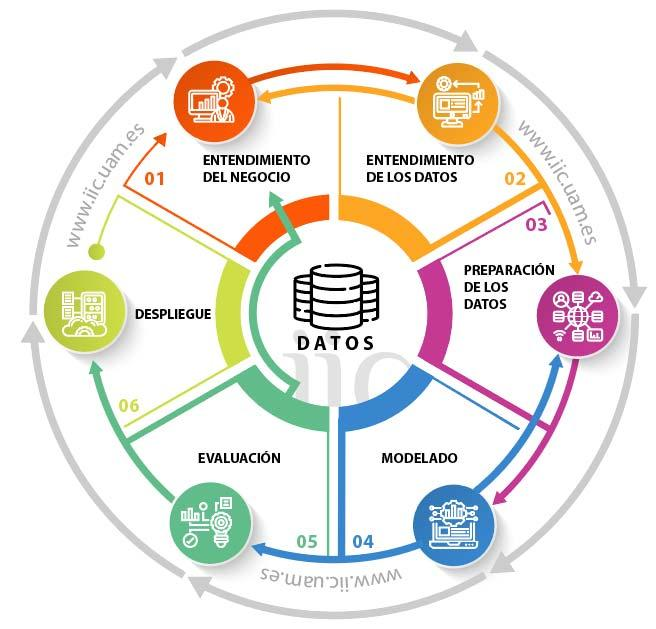
\includegraphics[width=0.8\textwidth]{./img/metodologia/crispdm.jpeg}
    \caption{Esquema del ciclo CRISP-DM estándar \cite{haya_crisp_dm}.}
    \label{fig:CRISP-DM}
\end{figure}

\section{SCRUM}

Un marco de trabajo ágil es una estructura metodológica utilizada para gestionar proyectos de manera flexible, iterativa y centrada en la entrega continua de valor. Estos marcos se basan en los principios del Manifiesto Ágil, el cual promueve la colaboración entre equipos multidisciplinarios, la respuesta rápida al cambio y la entrega frecuente de productos funcionales al cliente \cite{beck2001manifesto}.

Los marcos ágiles permiten a los equipos adaptarse a condiciones cambiantes y enfocarse en mejorar constantemente, promoviendo una comunicación fluida, ciclos de retroalimentación cortos y una participación activa del cliente durante todo el desarrollo del producto.

Dentro de estos marcos, uno de los más populares y ampliamente adoptados es Scrum. 

Scrum es un marco de trabajo ágil diseñado para ayudar a equipos a desarrollar productos complejos de forma incremental. Se caracteriza por su estructura liviana y fácil de entender, aunque su dominio completo requiere disciplina y experiencia. Scrum se basa en ciclos de trabajo cortos llamados \textit{sprints}, que típicamente duran entre una y cuatro semanas, durante los cuales se entrega un incremento funcional del producto. La Figura \ref{fig.SCRUM} muestra el ciclo de vida del marco de trabajo ágil scrum.

Este marco de trabajo ágil, establece roles definidos (\textit{Product Owner}, \textit{Scrum Master} y Equipo de Desarrollo), eventos específicos (como el \textit{Sprint}, la Planificación del \textit{Sprint}, la Revisión, la Retrospectiva y el \textit{Scrum} Diario) y artefactos clave \textit{(Product Backlog}, \textit{Sprint Backlog} e Incremento). Estos elementos promueven la transparencia, la inspección continua y la adaptación dentro del proceso de desarrollo.


\begin{figure}[H]
    \centering
    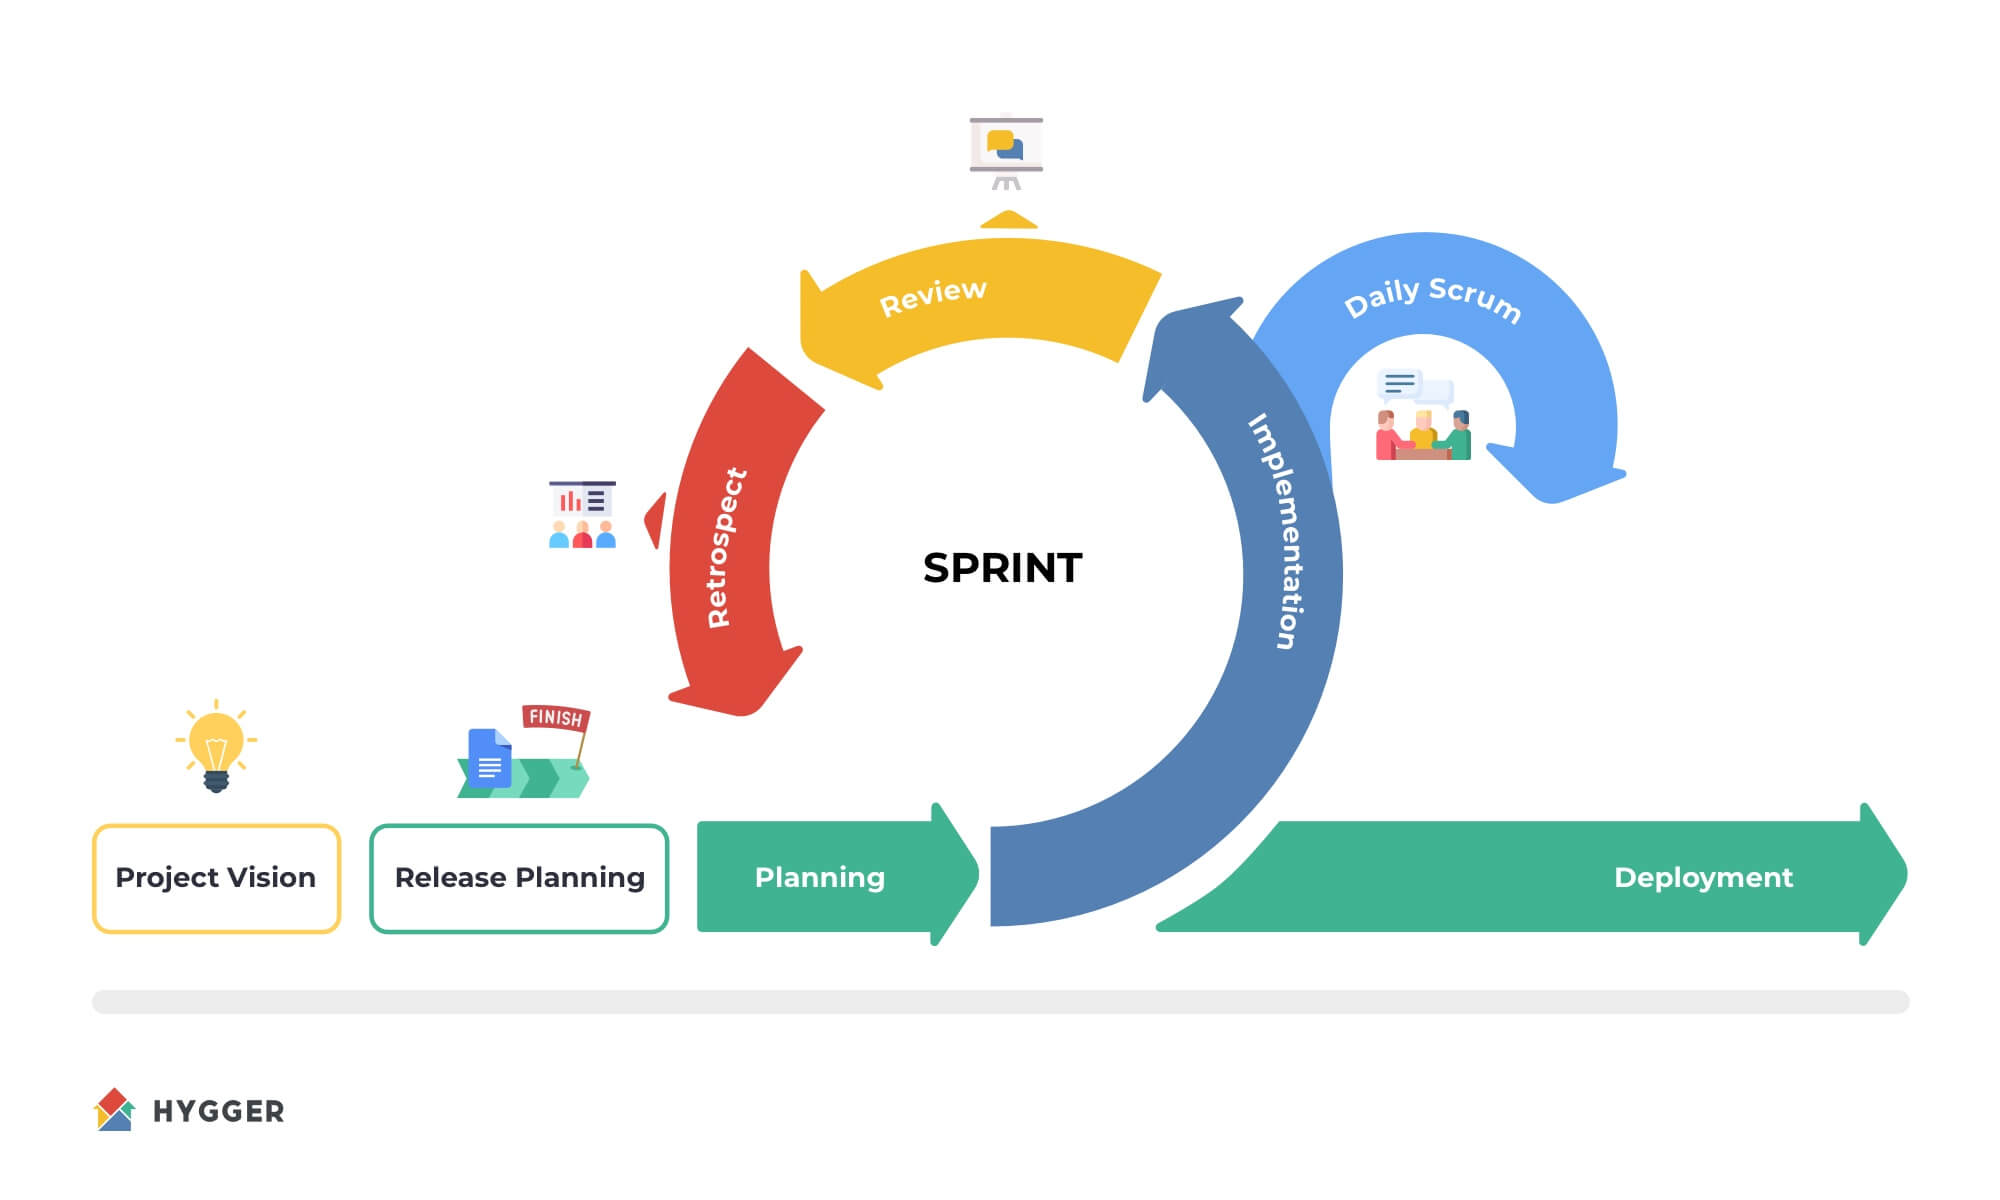
\includegraphics[width=0.8\textwidth]{./img/metodologia/scrum.jpg}
    \caption{Esquema del ciclo de vida de scrum \cite{schwaber2020scrum2}.}
    \label{fig.SCRUM}
\end{figure}



\chapter{Planificación}
Este capítulo aborda la organización detallada del trabajo de fin de grado, cubriendo desde su diseño inicial hasta la implementación y el seguimiento durante su desarrollo. Una planificación rigurosa resulta fundamental para sentar las bases del proyecto, ya que permite definir con claridad los objetivos, los recursos necesarios, los plazos de entrega y las actividades clave para alcanzar los resultados esperados \cite{pmbok}.

En primer lugar, se establece una planificación temporal preliminar, donde se estiman los tiempos requeridos para cada etapa. Este cronograma se estructura en torno a las fases de la metodología CRISP-DM, complementadas con etapas específicas propias de un Trabajo de Fin de Grado. A continuación, se realiza un análisis de riesgos exhaustivo, evaluando tanto la probabilidad como el impacto de cada posible contingencia.

Además, se elabora un presupuesto detallado para las tareas del proyecto, abordado desde dos perspectivas. Por un lado, se incluye una estimación realista de los costes asociados a la ejecución del trabajo en el ámbito académico. Por otro lado, se plantea una proyección teórica de los gastos que implicaría un proyecto equivalente en un contexto profesional.

Por último, se contrasta la planificación inicial con el desarrollo real del trabajo, lo que permite evaluar posibles desviaciones y los aprendizajes obtenidos durante el proceso.

\section{Planificación temporal}

La planificación temporal constituye un elemento fundamental en la ejecución de un proyecto fin de grado, ya que permite estructurar de manera sistemática todas las actividades necesarias para alcanzar los objetivos propuestos. En el contexto de un trabajo académico que combine el desarrollo de software con una metodología de investigación, como es el caso de CRISP-DM para el modelo de proceso y SCRUM para la gestión del proyecto, una adecuada planificación garantiza la distribución equilibrada del tiempo disponible entre las distintas fases del trabajo. Esta organización temporal resulta especialmente relevante cuando se deben coordinar aspectos teóricos, desarrollo técnico y validación de resultados, asegurando que cada componente reciba la atención necesaria sin comprometer la calidad global del proyecto.

El empleo de un diagrama de Gantt como herramienta de planificación ofrece ventajas significativas para visualizar la secuencia de actividades y su superposición temporal. Este tipo de representación gráfica facilita la identificación de hitos críticos y dependencias entre tareas, aspectos particularmente importantes cuando se combinan metodologías diferentes como CRISP-DM y SCRUM. La primera, con sus fases bien definidas, proporciona la estructura para el desarrollo del núcleo analítico del proyecto, mientras que SCRUM, con sus sprints iterativos, permite adaptar el trabajo a los descubrimientos que vayan surgiendo durante la investigación. La integración de ambas aproximaciones en un único cronograma exige una cuidadosa coordinación que el diagrama de Gantt ayuda a materializar de forma clara y comprensible. El diagrama de Gantt utilizado para la planificación de este trabajo se muestra en la Figura \ref{fig:gantt}. Este diagrama tiene una duración de 300 horas, que corresponden con las horas de trabajo de alumno de los 12 créditos ECTS que exige el plan de estudios del Grado de Ingeniería Informática de la UVa para el TFG.



\begin{figure}[H]
\centering
\makebox[\linewidth][c]{%  % Centrado mejorado
\begin{ganttchart}[
    x unit=0.15cm,         % Aumentado para ocupar más ancho
    y unit title=0.8cm,
    y unit chart=0.6cm,
    hgrid,
    vgrid={*{1}{dotted}},
    title/.style={draw=none},
    title label font=\footnotesize,
    bar/.style={fill=blue!30, rounded corners=2pt},
    bar height=0.6,
    group/.style={draw=black, fill=blue!10},
    milestone/.style={fill=red, rounded corners=2pt},
    bar label font=\scriptsize,
    group label font=\small,
    milestone label font=\scriptsize,
    expand chart=\linewidth  % Ocupa todo el ancho disponible
]{1}{90}
    % Título principal centrado sobre semanas
    \gantttitle{Diagrama de Gantt del Proyecto}{90} \\
    
    % Cabecera de semanas (13 semanas para 90 días)
    \gantttitlelist{1,2,3,4,5,6,7,8,9,10,11,12,13}{7} \\
    
    % Fases y tareas (igual que antes pero ajustadas visualmente)
    \ganttgroup{1. Comprensión Negocio}{1}{10} \\
    \ganttbar{1.1 Definición objetivos}{1}{5} \\
    \ganttbar{1.2 Análisis requisitos}{6}{10} \\
    
    \ganttgroup{2. Comprensión Datos}{11}{20} \\
    \ganttbar{2.1 Recopilación datos}{11}{15} \\
    \ganttbar{2.2 Análisis exploratorio}{16}{20} \\
    
    \ganttgroup{Sprint 1: Preparación}{21}{35} \\
    \ganttbar{3.1 Limpieza datos}{21}{25} \\
    \ganttbar{3.2 Feature engineering}{26}{30} \\
    \ganttbar{3.3 Normalización}{31}{35} \\
    \ganttmilestone{Hito 1}{35} \\
    
    \ganttgroup{Sprint 2: Modelado}{36}{60} \\
    \ganttbar{4.1 Selección algoritmos}{36}{40} \\
    \ganttbar{4.2 Entrenamiento inicial}{41}{50} \\
    \ganttbar{4.3 Ajuste parámetros}{51}{60} \\
    \ganttmilestone{Hito 2}{60} \\
    
    \ganttgroup{Sprint 3: Evaluación}{61}{80} \\
    \ganttbar{5.1 Validación cruzada}{61}{65} \\
    \ganttbar{5.2 Pruebas rendimiento}{66}{70} \\
    \ganttbar{5.3 Análisis resultados}{71}{80} \\
    \ganttmilestone{Hito 3}{80} \\
    
    \ganttgroup{6. Documentación}{81}{90} \\
    \ganttbar{6.1 Redacción memoria}{81}{85} \\
    \ganttbar{6.2 Preparación defensa}{86}{90} \\
    \ganttmilestone{Entrega Final}{90}
\end{ganttchart}
}
\caption{Diagrama de Gantt para la planificación del proyecto.}
\label{fig:gantt}
\end{figure}

\section{Gestión de riesgos}

En este apartado se presentan los principales riesgos potenciales del proyecto junto con sus correspondientes planes de mitigación. Además, en la Figura \ref{tab:hitos} se muestran las horas dedicadas al cumplimiento de cada hito del trabajo. De acuerdo con el PMBOK (\textit{Project Management Body of Knowledge}) \cite{pmbok}, los riesgos en gestión de proyectos se clasifican en las categorías de la sección \ref{subsec.tiprisks}.

\subsection*{Hitos del Proyecto}
\begin{table}[h]
\centering
\begin{tabular}{|l|c|c|}
\hline
\textbf{Hito} & \textbf{Horas hasta el hito} & \textbf{Horas acumuladas} \\ \hline
Finalización de formación y trabajos previos & 20 & 20 \\ \hline
Finalización de la planificación inicial & 30 & 50 \\ \hline
Finalización de la comprensión de datos & 40 & 90 \\ \hline
Finalización del modelado & 80 & 170 \\ \hline
Obtención de modelos óptimos & 40 & 210 \\ \hline
Finalización y entrega de la memoria & 90 & 300 \\ \hline
\end{tabular}
\caption{Cronograma de hitos y horas de trabajo.}
\label{tab:hitos}
\end{table}

\subsection*{Tipología de Riesgos} \label{subsec.tiprisks}
\begin{enumerate}
    \item \textbf{Riesgos Técnicos:}
    \begin{itemize}
        \item Limitaciones en la infraestructura de hardware.
        \item Incompatibilidad entre sistemas o tecnologías.
        \item Problemas de rendimiento o escalabilidad.        
        \item Deficiencias en el diseño o implementación de software.
    \end{itemize}
    
    \item \textbf{Riesgos de Gestión:}
    \begin{itemize}
        \item Deficiencias en la comunicación entre los miembros del equipo.
        \item Modificaciones en los requisitos del proyecto.        
        \item Inestabilidad del equipo por conflictos internos o rotación de personal.
        \item Retrasos en la disponibilidad de recursos críticos.

    \end{itemize}
    
    \item \textbf{Riesgos de Mercado:}
    \begin{itemize}
        \item Aparición de competencia no anticipada.
        \item Variaciones en las condiciones del mercado que afectan la demanda.
        \item Cambios regulatorios que impactan la ejecución del proyecto.
    \end{itemize}
    
    \item \textbf{Riesgos Financieros:}
    \begin{itemize}
        \item Limitaciones en la disponibilidad de fondos.
        \item Excesos presupuestarios no previstos.
        \item Fluctuaciones en los tipos de cambio.
    \end{itemize}
    
    \item \textbf{Riesgos Externos:}
    \begin{itemize}
        \item Fenómenos meteorológicos adversos.
        \item Interrupciones en la cadena de suministro.
        \item Eventos naturales catastróficos.
    \end{itemize}
\end{enumerate}

\subsection*{Metodología de Evaluación}
La identificación y valoración de riesgos se realiza mediante criterios cualitativos, al no disponer de métricas cuantitativas suficientemente fiables para un análisis más exhaustivo. Este enfoque permite priorizar los riesgos según su impacto potencial y probabilidad de ocurrencia \cite{carmona2021gestion}.

\begin{table}[H]
\centering
\begin{tabular}{|>{\hsize=1.1\hsize}c|>{\hsize=1.1\hsize}c|c|c|c|c|c|}
\hline
\rowcolor{gray!25}
\multicolumn{2}{|c|}{\multirow{2}{*}{}} & \multicolumn{5}{c|}{\textbf{Impacto}} \\
\cline{3-7}
\multicolumn{2}{|c|}{} & \textbf{Mínimo} & \textbf{Bajo} & \textbf{Medio} & \textbf{Alto} & \textbf{Extremo} \\ \hline

\multirow{6}{*}{\rotatebox{90}{\textbf{Probabilidad}}} 
& \textbf{Extrema} & \cellcolor{greenrisk} & \cellcolor{yellowrisk} & \cellcolor{orangerisk} & \cellcolor{redrisk} & \cellcolor{redrisk} \\ \cline{2-7}
& \textbf{Alta} & \cellcolor{greenrisk} & \cellcolor{greenrisk} & \cellcolor{yellowrisk} & \cellcolor{orangerisk} & \cellcolor{redrisk} \\ \cline{2-7}
& \textbf{Media} & \cellcolor{bluerisk} & \cellcolor{greenrisk} & \cellcolor{greenrisk} & \cellcolor{yellowrisk} & \cellcolor{orangerisk} \\ \cline{2-7}
& \textbf{Baja} & \cellcolor{bluerisk} & \cellcolor{bluerisk} & \cellcolor{greenrisk} & \cellcolor{greenrisk} & \cellcolor{yellowrisk} \\ \cline{2-7}
& \textbf{Muy Baja} & \cellcolor{bluerisk} & \cellcolor{bluerisk} & \cellcolor{bluerisk} & \cellcolor{greenrisk} & \cellcolor{greenrisk} \\ \hline
\end{tabular}

\vspace{5mm}

\begin{tabular}{|l|l|}
\hline
\rowcolor{gray!25}
\textbf{Nivel de Riesgo} & \textbf{Color} \\ \hline
Extremo & \cellcolor{redrisk} \\ \hline
Alto & \cellcolor{orangerisk} \\ \hline
Moderado & \cellcolor{yellowrisk} \\ \hline
Bajo & \cellcolor{greenrisk} \\ \hline
Mínimo & \cellcolor{bluerisk} \\ \hline
\end{tabular}
\caption{Matriz Probabilidad-Impacto.}
\label{tab:matrizpi}
\end{table}

\begin{description}[leftmargin=1cm, style=nextline]

\item[\textbf{Probabilidad}]
Grado de posibilidad de que un riesgo se materialice. Se suele cuantificar en escala del 1 (muy improbable) al 5 (casi seguro). En la matriz que se muestra en la Tabla \ref{tab:matrizpi}, determina el eje vertical y se combina con el impacto para priorizar riesgos.

\item[\textbf{Impacto}]
Consecuencia o efecto potencial que tendría la materialización del riesgo. Se valora del 1 (impacto mínimo) al 5 (impacto catastrófico). Representa en la matriz que se muestra en la Tabla \ref{tab:matrizpi}, el eje horizontal en la matriz y mide la severidad del riesgo.

\item[\textbf{Plan de Mitigación}]
Acciones proactivas para reducir la probabilidad o impacto del riesgo antes de que ocurra. Incluye:
\begin{itemize}
\item Prevención: Eliminar las causas del riesgo.
\item Reducción: Disminuir su probabilidad o impacto.
\item Transferencia: Trasladar el riesgo a terceros.
\end{itemize}

\item[\textbf{Plan de Contingencia}]
Medidas reactivas que se implementan cuando el riesgo se materializa. Contiene:
\begin{itemize}
\item Activación: Criterios para ejecutar el plan.
\item Respuesta: Acciones específicas de contención.
\item Recuperación: Cómo volver a la normalidad.
\end{itemize}

\item[\textbf{Nivel de Riesgo}]
Resultado de multiplicar la probabilidad por el impacto. Clasifica riesgos en:
\begin{itemize}
\item Alto (15-25): Requieren acción inmediata.
\item Medio (5-14): Necesitan monitoreo.
\item Bajo (1-4): Aceptables con supervisión mínima.
\end{itemize}

\item[\textbf{Umbral de Riesgo}]
Límite máximo aceptable de riesgo para el proyecto. Determina cuándo se deben implementar planes de mitigación o contingencia.

\item[\textbf{Propietario del Riesgo}]
Persona o equipo responsable de monitorear cada riesgo y ejecutar los planes correspondientes.

\end{description}


\subsection*{Riesgos identificados}
\begin{enumerate}
    \item \textbf{R01}: Conflicto con periodos de exámenes y entregas de otras asignaturas (Tabla \ref{tab:R01}).
    \item \textbf{R02}: Fallos hardware en equipos de desarrollo (Tabla \ref{tab:R02}).
    \item \textbf{R03}: Limitaciones de capacidad de procesamiento para el entrenamiento de los modelos (Tabla \ref{tab:R03}).
    \item \textbf{R04}: Pérdida o corrupción del código (Tabla \ref{tab:R04}).
    \item \textbf{R05}: Disponibilidad limitada del tutor académico (Tabla \ref{tab:R05}).
    \item \textbf{R06}: Desviaciones en la planificación temporal inicial (Tabla \ref{tab:R06}).
    \item \textbf{R07}: Cambios en los requisitos técnicos (Tabla \ref{tab:R07}).
    \item \textbf{R08}: Interpretación errónea de los resultados por falta de formazión en técnicas de aprendizaje automático. (Tabla \ref{tab:R08}).
    \item \textbf{R09}: Problemas de licencias de software (Tabla \ref{tab:R09}).
\end{enumerate}

% Riesgo R01
\begin{table}[H]
\centering
\begin{tabular}{|>{\bfseries}l|p{10cm}|}
\hline
\rowcolor{lightgray}
\multicolumn{2}{|c|}{\textbf{Riesgo R01}} \\ \hline
Título & Conflicto con periodos de exámenes y entregas de otras asignaturas.\\ \hline
Descripción & Sobrecarga académica que dificulta la dedicación y el rendimiento en todas las tareas. \\ \hline
Probabilidad & 4 (Alta) \cellcolor{orangerisk} \\ \hline
Impacto & 3 (Media) \cellcolor{yellowrisk}\\ \hline
Matriz P/I & Alta/Media (12)\\ \hline
Plan Mitigación & 
\begin{itemize}
\item Coordinar calendario académico anticipadamente.
\item Avanzar trabajo en periodos de menor carga de trabajo.
\end{itemize} \\ \hline
Plan Contingencia & 
\begin{itemize}
\item Dedicar horas extra en los asuntos académicos.
\item Reorganizar prioridades temporales.
\end{itemize} \\ \hline
\end{tabular}
\caption{R01: Conflicto con periodos de exámenes y entregas de otras asignaturas.}
\label{tab:R01}
\end{table}


% Riesgo R02
\begin{table}[H]
\centering
\begin{tabular}{|>{\bfseries}l|p{10cm}|}
\hline
\rowcolor{lightgray}
\multicolumn{2}{|c|}{\textbf{Riesgo R02}} \\ \hline
Título & Fallos hardware en equipos de desarrollo. \\ \hline
Descripción & Problemas causados por el mal funcionamiento de los componentes físicos de un ordenador, como la placa base, la tarjeta gráfica, la memoria RAM, el disco duro o la fuente de alimentación en equipos de desarrollo. \\ \hline
Probabilidad & 3 (Media)   \cellcolor{yellowrisk}\\ \hline
Impacto & 4 (Alto)   \cellcolor{orangerisk}\\ \hline
Matriz P/I & Media/Alto (12)\\ \hline
Plan Mitigación & 
\begin{itemize}
\item Mantenimiento preventivo mensual.
\item Uso de equipos redundantes.
\end{itemize} \\ \hline
Plan Contingencia & 
\begin{itemize}
\item Utilizar equipos alternativos.
\item Uso de máquinas virtuales del sistema de virtualización de la Escuela de Ingeniería de Informática de Valladolid.
\end{itemize} \\ \hline
\end{tabular}
\caption{R02: Fallos hardware en equipos de desarrollo.}
\label{tab:R02}
\end{table}

% Riesgo R03
\begin{table}[H]
\centering
\begin{tabular}{|>{\bfseries}l|p{10cm}|}
\hline
\rowcolor{lightgray}
\multicolumn{2}{|c|}{\textbf{Riesgo R03}} \\ \hline
Título & Limitaciones de capacidad de procesamiento para el entrenamiento de los modelos. \\ \hline
Descripción & Restricciones de hardware (cálculo, memoria) que impactan la velocidad, viabilidad y calidad del entrenamiento, influyendo en el tamaño y complejidad de los modelos.\\ \hline
Probabilidad & 4 (Alta)   \cellcolor{orangerisk}\\ \hline
Impacto & 5 (Extremo)  \cellcolor{redrisk}\\ \hline
Matriz P/I & Alto/Extremo (20)\\ \hline
Plan Mitigación & 
\begin{itemize}
\item Optimización temprana del código.
\item Uso de técnicas de muestreo.
\end{itemize} \\ \hline
Plan Contingencia & 
\begin{itemize}
\item Utilizar sistema de virtualización de la escuela
\item Reducir complejidad de modelos.
\end{itemize} \\ \hline
\end{tabular}
\caption{R03: Limitaciones de capacidad de procesamiento para el entrenamiento de los modelos.}
\label{tab:R03}
\end{table}

% Riesgo R04
\begin{table}[H]
\centering
\begin{tabular}{|>{\bfseries}l|p{10cm}|}
\hline
\rowcolor{lightgray}
\multicolumn{2}{|c|}{\textbf{Riesgo R04}} \\ \hline
Título & Pérdida o corrupción del código. \\ \hline
Descripción & Extraviación o daño en los conjuntos de datos del proyecto que se utilizan para en entrenamiento y la validación del modelo.\\ \hline
Probabilidad & 2 (Baja)  \cellcolor{greenrisk}\\ \hline
Impacto & 5 (Extremo) \cellcolor{redrisk}\\ \hline
Matriz P/I & Baja/Extremo (10) \\ \hline
Plan Mitigación & 
\begin{itemize}
\item Almacenamiento redundante de los datos en repositorios.
\item Verificación de la inegridad de los datos con checksums.
\end{itemize} \\ \hline
Plan Contingencia & 
\begin{itemize}
\item Recuperar datasets desde backups externos.
\item Regenerar datos sintéticos.
\end{itemize} \\ \hline
\end{tabular}
\caption{R04: Pérdida o corrupción del código.}
\label{tab:R04}
\end{table}

% Riesgo R05
\begin{table}[H]
\centering
\begin{tabular}{|>{\bfseries}l|p{10cm}|}
\hline
\rowcolor{lightgray}
\multicolumn{2}{|c|}{\textbf{Riesgo R05}} \\ \hline
Título & Disponibilidad limitada del tutor académico.\\ \hline
Descripción & Restricciones de tiempo y acceso al tutor académico, afectando la frecuencia y profundidad de la retroalimentación y el apoyo al estudiante en su proceso de aprendizaje. \\ \hline
Probabilidad & 3 (Media) \cellcolor{yellowrisk}\\ \hline
Impacto & 3 (Media) \cellcolor{yellowrisk}\\ \hline
Matriz P/I & Media/Media (9)\\ \hline
Plan Mitigación & 
\begin{itemize}
\item Agendar reuniones con anticipación.
\item Preparar preguntas concretas.
\end{itemize} \\ \hline
Plan Contingencia & 
\begin{itemize}
\item Consultar con profesores alternativos.
\item Usar foros académicos.
\end{itemize} \\ \hline
\end{tabular}
\caption{R05: Disponibilidad limitada del tutor académico.}
\label{tab:R05}
\end{table}

% Riesgo R06
\begin{table}[H]
\centering
\begin{tabular}{|>{\bfseries}l|p{10cm}|}
\hline
\rowcolor{lightgray}
\multicolumn{2}{|c|}{\textbf{Riesgo R06}} \\ \hline
Título & Desviaciones en la planificación temporal inicial. \\ \hline
Descripción & Variaciones o retrasos respecto al cronograma original, impactando los plazos de entrega, la gestión del tiempo y la consecución de los objetivos previstos. \\ \hline
Probabilidad & 4 (Alta) \cellcolor{orangerisk}\\ \hline
Impacto & 4 (Alto) \cellcolor{orangerisk}\\ \hline
Matriz P/I & Alto/Alto (16)\\ \hline
Plan Mitigación & 
\begin{itemize}
\item Incluir días asignados a descanso como días dedicados al proyecto.
\item Revisiones semanales de progreso.
\end{itemize} \\ \hline
Plan Contingencia & 
\begin{itemize}
\item Reorganizar del diagrama de Gantt.
\item Eliminar funcionalidades no críticas.
\end{itemize} \\ \hline
\end{tabular}
\caption{R06: Desviaciones en la planificación temporal inicial.}
\label{tab:R06}
\end{table}

% Riesgo R07
\begin{table}[H]
\centering
\begin{tabular}{|>{\bfseries}l|p{10cm}|}
\hline
\rowcolor{lightgray}
\multicolumn{2}{|c|}{\textbf{Riesgo R07}} \\ \hline
Título & Cambios en los requisitos técnicos. \\ \hline
Descripción &  Modificaciones o alteraciones en las especificaciones necesarias para un proyecto o tarea, que pueden afectar al diseño, a la implementación, a los recursos y a los plazos. \\ \hline
Probabilidad & 4 (Alta)  \cellcolor{orangerisk}\\ \hline
Impacto & 4 (Alto) \cellcolor{orangerisk}\\ \hline
Matriz P/I & Alto/Alto (16)\\ \hline
Plan Mitigación & 
\begin{itemize}
\item Documentar requisitos iniciales con precisión.
\item Establecer procedimiento de cambio formal.
\end{itemize} \\ \hline
Plan Contingencia & 
\begin{itemize}
\item Revisar el alcance con tutor.
\item Asignar tiempo adicional para cambios.
\end{itemize} \\ \hline
\end{tabular}
\caption{R07: Cambios en los requisitos técnicos.}
\label{tab:R07}
\end{table}

% Riesgo R08
\begin{table}[H]
\centering
\begin{tabular}{|>{\bfseries}l|p{10cm}|}
\hline
\rowcolor{lightgray}
\multicolumn{2}{|c|}{\textbf{Riesgo R08}} \\ \hline
Título & Interpretación errónea de los resultados por falta de formazión en técnicas de aprendizaje automático.  \\ \hline
Descripción & El desconocimiento de las métricas utilizadas para analizar los resutlados como precisión, recall, F1, puede llevar a confiar en modelos con bajo desempeño real o tomar decisiones equivocadas basadas en correlaciones espurias. \\ \hline
Probabilidad & 3 (Media) \cellcolor{yellowrisk} \\ \hline
Impacto & 5 (Extremo) \cellcolor{redrisk} \\ \hline
Matriz P/I & Media/Extremo (15) \\ \hline
Plan Mitigación & 
\begin{itemize}
\item Buscar alternativas para obtener una formación básica en técnicas de aprendizaje automático.
\item Corroborar los resultados obtenidos con el tutor académico.
\end{itemize} \\ \hline
Plan Contingencia & 
\begin{itemize}
\item Suspender de manera inmediata las decisiones tomadas basadas en las salidas mal interpretadas del modelo.
\item Reemplazar el modelo mal interpretado por una versión anterior o un modelo base.
\end{itemize} \\ \hline
\end{tabular}
\caption{R08: Dependencia de tecnologías inestables o no documentadas.}
\label{tab:R08}
\end{table}

% Riesgo R09
\begin{table}[H]
\centering
\begin{tabular}{|>{\bfseries}l|p{10cm}|}
\hline
\rowcolor{lightgray}
\multicolumn{2}{|c|}{\textbf{Riesgo R09}} \\ \hline
Título & Problemas de licencia de software.\\ \hline
Descripción & Inconvenientes o restricciones legales relacionadas con el uso, la distribución o la activación de software, pudiendo causar interrupciones, costos adicionales o incluso acciones legales. \\ \hline
Probabilidad & 2 (Baja) \cellcolor{greenrisk} \\ \hline
Impacto & 3 (Media)  \cellcolor{yellowrisk}\\ \hline
Matriz P/I & Baja/Media (6)\\ \hline
Plan Mitigación & 
\begin{itemize}
\item Verificar licencias antes de usarlas para su implementación.
\item Priorizar la utilización software open-source.
\end{itemize} \\ \hline
Plan Contingencia & 
\begin{itemize}
\item Buscar alternativas equivalentes.
\item Solicitar licencias académicas.
\end{itemize} \\ \hline
\end{tabular}
\caption{R09: Problemas de licencia de software.}
\label{tab:R09}
\end{table}


\section{Estimación de costes}
En esta sección se presenta la estimación de costes, que comprende la identificación y valoración de los recursos necesarios para el desarrollo del proyecto. Este proceso implica la cuantificación de los gastos previsibles asociados a materiales y software específico utilizado. También se considera un coste el tiempo dedicado por el estudiante a la realización del trabajo.

La precisión en la estimación de costes facilita la elaboración de un presupuesto realista y la planificación financiera del proyecto. Permite anticipar las necesidades económicas, buscar posibles fuentes de financiación si fuese necesario y gestionar eficientemente los recursos disponibles. Una estimación detallada contribuye a evitar desviaciones presupuestarias y a asegurar la viabilidad económica del proyecto \cite{oliveros2011gestion}.

\subsection{Costes materiales}
A continuación, se hace un recuento de los costes materiales en hardware y software que han sido utilizados para el desarrollo de este proyecto.
\subsection*{Hardware}
El hardware comprende el conjunto de componentes físicos y tangibles que constituyen un sistema informático. Proporciona la infraestructura física necesaria para la ejecución del software y el procesamiento de la información.

Para realizar este proyecto se ha utilizado un equipo informático con los siguientes componentes:
\begin{itemize}
\item \textbf{CPU}: AMD Ryzen 7 6800HS with Radeon Graphics (16) @ 4.785GHz
\item \textbf{RAM}: 16GB SO-DIMM DDR5 4800MH
\item \textbf{Memoria}: 512GB PCIe® 4.0 NVMe™ M.2 SSD
\item \textbf{GPU1}: NVIDIA GeForce RTX 3050 Mobile 
\item \textbf{GPU2}: AMD ATI Radeon 680M
\end{itemize}

Debido al tamaño del conjunto de datos, el componente que más ha ralentizado el proyecto es la RAM, que en ciertas ocasiones durante el entrenamiento de los modelos se quedaba algo escasa en capacidad.

Teniendo en cuenta que el coste del ordenador en el momento de la compra fue de 829\,€, que la vida útil aproximada es de 8 años y que para el desarrollo de este proyecto se ha estado utilizando durante 3,5 meses, la amortización del hardware es:

\begin{equation}
	\text{Amortización del Hardware} = 829\,\text{€} \times \frac{1}{8} \times \frac{3.5}{12} = 30,22\,\text{€}
\end{equation}

\subsection*{Software}
El software constituye el conjunto intangible de programas, datos e instrucciones que habilitan el funcionamiento de un sistema informático. Es el responsable de definir la funcionalidad, el comportamiento y la interacción del sistema con el usuario y con otros sistemas. En la Tabla \ref{tab:costes_software} se detalla el coste del software utilizado para desarrollar este trabajo.

\begin{table}[H]
\centering
\begin{tabular}{|l|l|c|c|c|}
\toprule
Funcionalidad & Software & Coste Mensual & Duración & Coste Total \\
\midrule
Sistema Operativo (SO) & Kubuntu 24.10 x86\_64  & 0\,€  & 3,5 meses & 0\,€ \\
Lenguaje (memoria) & Latex &  0\,€ & 3 meses & 0\,€ \\
Editor latex & TexMaker & 0\,€ & 3 meses & 0\,€ \\
IDE  & MS Visual Studio Code & 0\,€ & 1 mes & 0\,€ \\
Lenguaje (modelos) & Python & 0\,€ & 1 mes & 0\,€ \\
IDE de Python & Jupyeter Notebooks & 0\,€ & 1 mes & 0\,€ \\
Plataforma MLOps\footnote{Machine Learning Operations, son un conjunto de prácticas y principios que buscan gestionar de forma eficiente y escalable el ciclo de vida del aprendizaje automático} & Weights\&Biases & 0\,€ & 1 mes & 0\,€ \\
Control de versiones & GitHub & 0\,€ & 1 mes & 0\,€ \\
IA generativa (código) & DeepSeek & 0\,€ & 1 mes & 0\,€ \\
IA generativa (memoria) & Gemini & 0\,€ & 2 mes & 0\,€ \\
Comunicación 1 & MS Outlook & 0\,€ \footnote{licencia académica} & 3,5 mes & 0\,€ \\
Comunicación 2 & MS Teams & 0\,€ & 3,5 mes & 0\,€ \\
\bottomrule
\end{tabular}
\caption{Costes de Software.}
\label{tab:costes_software}
\end{table}

Debido a que el proyecto se realiza en un ámbito académico, se han minimizado los costes software del proyecto utilizando exclusivamente herramientas cedidas por la entidad académica o bien herramientas con licencia open-source que no suponen un coste monetario para el desarrollo del proyecto. 


\subsection{Costes humanos} \label{subsec.costeshumanos}
Como proyecto académico, los costes humanos representan el valor del tiempo y el esfuerzo personal invertido en la planificación, investigación, redacción y presentación del trabajo. Estos costes se manifiestan en las horas dedicadas al proyecto, el esfuerzo intelectual requerido, el aplazamiento o anulación de otras actividades personales o profesionales y el estrés asociado al proceso.

En el caso de la simulación de los costes monetarios de un proyecto similar a este, sería necesario contar con personas cualificadas para los siguientes puestos:
\begin{itemize}
\item Ingeniero de Aprendizaje Automático.
\item Cientifico de Datos.
\item Analista de Satos.
\end{itemize}

Los costes humanos se dividen en tres fases diferentes:
\begin{enumerate}
	\item Definición y Preparación: la Tabla \ref{tab:costes_fase1} muestra los costes para esta fase.
	\item Desarrollo y Entrenamiento: los costes para esta fase vienen desarrollados en la Tabla \ref{tab:costes_fase2}.
	\item Definición y Preparación: la Tabla \ref{tab:costes_fase3} detalla los costes de esta fase del proyecto.
\end{enumerate}

Para obtener una visión de conjunto de los costes humanos del proyecto, la Tabla \ref{tab:coste_total_profesional} refleja la suma de las fases comentadas.


\subsubsection*{Fase 1: Definición y Preparación (75 horas)}
\begin{table}[H]
\centering
\begin{tabular}{|l|c|c|c|}
\toprule
Profesional & €/hora & Horas & Total (€) \\
\midrule
Ingeniero ML & 42 & 12 & 504 \\
Científico Datos & 34,5 & 38 & 1\,311 \\
Analista Datos & 18,5 & 25 & 462,5 \\
\midrule
\textbf{Total Fase 1} & & \textbf{75} & \textbf{2\,277,5} \\
\bottomrule
\end{tabular}
\caption{Costes de Profesionales - Fase 1.}
\label{tab:costes_fase1}
\end{table}


\subsubsection*{Fase 2: Desarrollo y Entrenamiento (150 horas)}
\begin{table}[H]
\centering
\begin{tabular}{|l|c|c|c|}
\toprule
Profesional & €/hora & Horas & Total (€) \\
\midrule
Ingeniero ML & 42 & 95 & 3\,990 \\
Científico Datos & 34,5 & 38 & 1\,311 \\
Analista Datos & 18,5 & 17 & 314,5 \\
\midrule
\textbf{Total Fase 2} & & \textbf{150} & \textbf{5\,615,5} \\
\bottomrule
\end{tabular}
\caption{Costes de Profesionales - Fase 2.}
\label{tab:costes_fase2}
\end{table}


\subsubsection*{Fase 3: Validación y Evaluación (75 horas)}
\begin{table}[H]
\centering
\begin{tabular}{|l|c|c|c|}
\toprule
Profesional & €/hora & Horas & Total (€) \\
\midrule
Ingeniero ML & 42 & 30 & 1\,260 \\
Científico Datos & 34,5 & 37 & 1\,276,5 \\
Analista Datos & 18,5 & 8 & 148 \\
\midrule
\textbf{Total Fase 3} & & \textbf{75} & \textbf{2\,684,5} \\
\bottomrule
\end{tabular}
\caption{Costes de Profesionales - Fase 3.}
\label{tab:costes_fase3}
\end{table}

\subsubsection*{Coste Total del Proyecto (300 horas)}
\begin{table}[H]
\centering
\begin{tabular}{|l|c|}
\toprule
Profesional & Coste Total (€) \\
\midrule
Ingeniero ML & 5\,754 \\
Científico Datos & 3\,898,5 \\
Analista Datos & 925 \\
\midrule
\textbf{Coste Total del Proyecto} & \textbf{10\,577,5} \\
\bottomrule
\end{tabular}
\caption{Coste Total por Profesional}
\label{tab:coste_total_profesional}
\end{table}


Las estimaciones salariales proporcionadas se basan en los salarios en el sector tecnológico y de análisis de datos en España. Esta información se encuentra publicada en portales de empleo (Talent.com\footnote{https://es.talent.com/}), escuelas de negocio (Aicad Business School\footnote{https://www.aicad.es/}, KSchool\footnote{https://kschool.com/}, Esden Business School\footnote{https://esden.es/}) y noticias del sector (Tokio School\footnote{https://www.tokioschool.com/}). 










\label{cap.req-planificacion}

\chapter{Entendimiento del problema}
En este capítulo se trata el entendimiento del problema. Tal y como se comenta en el capítulo dos, es la fase inicial de la metología CRISP-DM. A continuación, se alinean los objetivos técnicos con las necesidades del negocio y con el problema a resolver. Se definen requisitos, se identifican métricas de éxito y se trata de dar comprensión sobre el contexto organizacional.


\section{¿Qué es un ataque a un sistema informático?}
Un ataque a un sistema informático constituye una acción deliberada y no autorizada que explota vulnerabilidades con el objetivo de comprometer la confidencialidad, integridad o disponibilidad de los datos y recursos del sistema. Esta actividad maliciosa puede manifestarse a través de diversas técnicas, incluyendo la inyección de código malicioso, la denegación de servicio, el acceso no autorizado y la ingeniería social. Su ejecución busca obtener beneficios ilícitos, interrumpir operaciones o dañar la infraestructura tecnológica.

La consecuencia de un ataque puede variar desde la pérdida o alteración de información sensible hasta la paralización completa de los servicios ofrecidos por el sistema. La identificación, análisis y mitigación de estas amenazas representan un aspecto fundamental en la seguridad informática, requiriendo la implementación de medidas preventivas y reactivas para proteger los activos digitales de una organización o individuo.

\section{Tipos de ataque a sistemas informáticos}


\section{¿Qué es TCP?}

El Protocolo de Control de Transmisión (TCP) constituye uno de los protocolos fundamentales de la capa de transporte del modelo TCP/IP, sobre el cual se sustenta gran parte de la comunicación en redes IP, incluyendo Internet. Su diseño se orienta a proporcionar un servicio de transferencia de datos fiable, ordenado y con detección de errores entre aplicaciones que se ejecutan en sistemas finales diferentes. Para lograr esta fiabilidad, TCP establece una conexión virtual punto a punto entre las aplicaciones comunicantes mediante un proceso de "three-way handshake", lo que permite la negociación de parámetros de la conexión y la sincronización de los números de secuencia iniciales.

\begin{figure}[htbp]
    \centering
    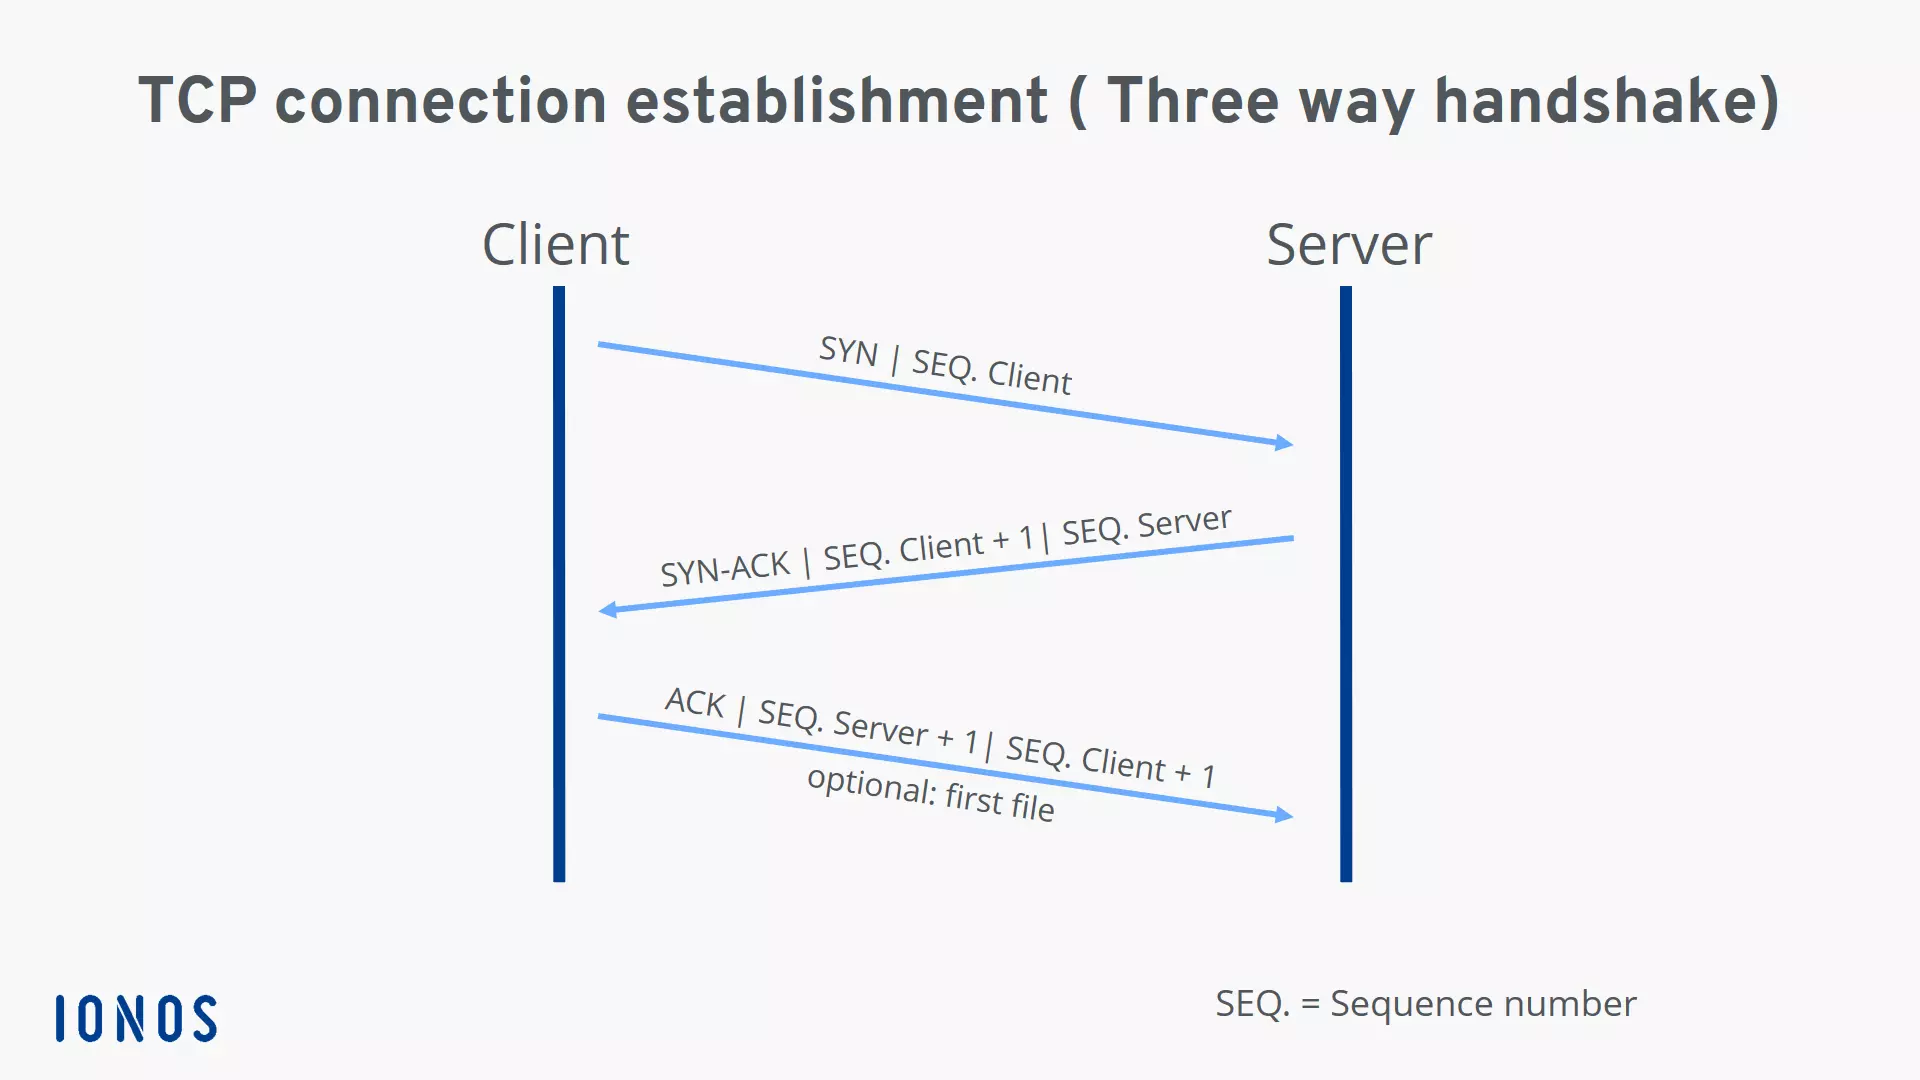
\includegraphics[width=0.8\textwidth]{./img/ent-problema/EsquemaTCP.png}
    \caption{Esquema funcionamiento TCP. \cite{tcpprotocolionos}}
    \label{fig:EsquemaTCP}
\end{figure}

El protocolo garantiza la entrega ordenada de la información al receptor mediante la asignación de números de secuencia a cada byte transmitido, permitiendo así la reordenación en caso de que la información no llegue al receptor en el orden correcto. La fiabilidad se logra a través de un mecanismo de acuse de recibo (acknowledgment, ACK) positivo con retransmisión, donde el receptor confirma la recepción correcta de los paquetes de información, y el emisor retransmite aquellos partes de la información para los que no recibe confirmación dentro de un tiempo límite (timeout).

\subsection{¿Qué es un segmento TCP?}
Una vez establecida la conexión, TCP divide los datos de la aplicación en unidades más pequeñas denominadas segmentos. Un segmento o paquete TCP constituye la unidad de datos fundamental que se intercambia a través de una red utilizando el mencionado protocolo TCP. Este segmento encapsula una porción de los datos de la capa de aplicación, precedida por una cabecera TCP. 

La cabecera TCP contiene información de control esencial para la funcionalidad del protocolo, incluyendo los números de puerto de origen y destino que identifican las aplicaciones comunicantes, los números de secuencia y de acuse de recibo (ACK) que garantizan la entrega ordenada y fiable, las banderas de control que indican el propósito del segmento (establecimiento de conexión, finalización, ACK, entre otros muchos), y otros campos como la ventana de recepción para el control de flujo y la suma de verificación para la detección de errores.


\begin{figure}[htbp]
    \centering
    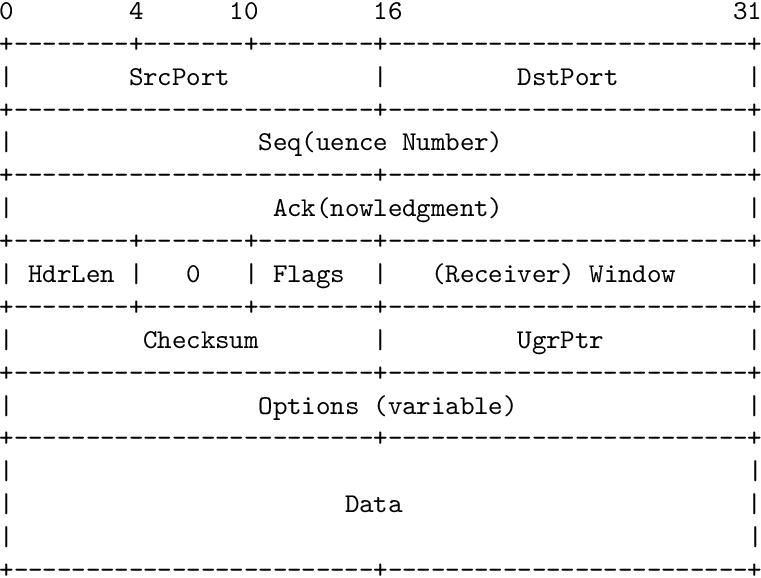
\includegraphics[width=0.8\textwidth]{./img/ent-problema/SegmentoTCP.png}
    \caption{Esquema segmento TCP. \cite{tcpsegment}}
    \label{fig:SegmentoTCP}
\end{figure}

En el proceso de transmisión, el segmento TCP se encapsula a su vez dentro de un paquete IP (Protocolo de Internet) para su enrutamiento a través de la red. El paquete IP añade su propia cabecera con las direcciones IP de origen y destino, entre otra información necesaria para el transporte a nivel de red. 

\begin{figure}[htbp]
    \centering
    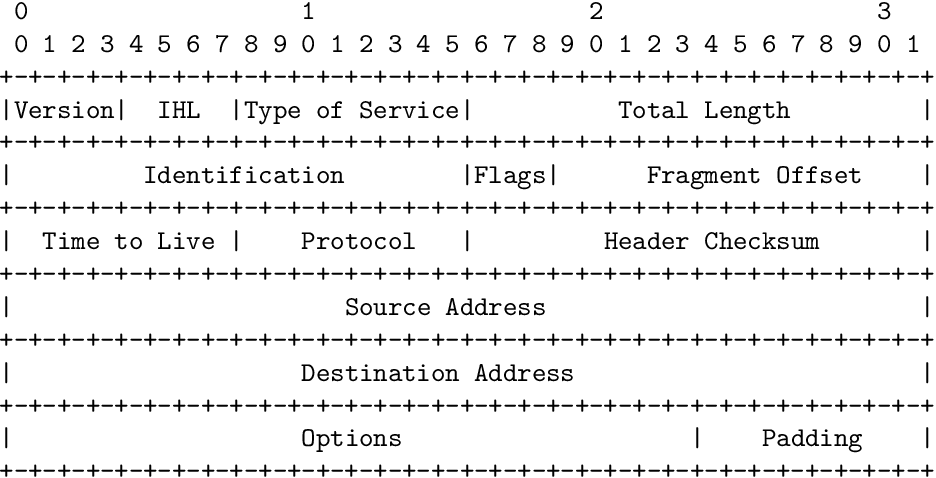
\includegraphics[width=0.8\textwidth]{./img/ent-problema/PaqueteIP.png}
    \caption{Formato de la cabecera en IPv4. \cite{paqueteip}}
    \label{fig:PaqueteIP}
\end{figure}

\section{Importancia de protegerse frente a un ataque}

La importancia de protegerse frente a ataques informáticos radica en la salvaguarda de activos digitales críticos, la garantía de la continuidad operativa y la preservación de la confianza y la reputación. En un entorno digital cada vez más interconectado, los ataques informáticos representan una amenaza significativa para individuos, organizaciones y la sociedad en su conjunto, pudiendo acarrear consecuencias devastadoras.

Para las organizaciones, las implicaciones de un ataque informático pueden ser aún más costosas. Estas implicaciones incluyen pérdidas financieras directas debido al robo de fondos, la interrupción de las operaciones comerciales, los costes de recuperación y las posibles sanciones regulatorias. Además, se puede producir un daño significativo a la reputación y la pérdida de la confianza de los clientes, lo que a largo plazo afecta la viabilidad del negocio. Los ataques también pueden resultar en el robo de propiedad intelectual, secretos comerciales e información estratégica, otorgando ventajas competitivas a adversarios. 

Por otra parte, la interrupción de servicios críticos, como energía, comunicaciones o sanidad, puede tener consecuencias graves para la sociedad en su conjunto.

La protección frente a ataques informáticos no es solo una cuestión de seguridad tecnológica, sino una necesidad imperante en la actualidad para proteger activos valiosos, asegurar la continuidad de las actividades, mantener la confianza de los usuarios y garantizar la estabilidad y el bienestar en el mundo digital actual. La implementación de prácticas de seguridad robustas y la concienciación sobre las amenazas cibernéticas son fundamentales en a la hora de defenderse de estos ataques.


\section{Importancia de detectar los ataques rápidamente}

La detección temprana de ataques informáticos constituye un pilar fundamental en la ciberseguridad moderna debido a su capacidad para mitigar consecuencias críticas. Cuando un sistema logra identificar intrusiones o actividades maliciosas en sus fases iniciales, se reducen significativamente los daños operativos y económicos. Esta rapidez de respuesta permite contener amenazas antes de que comprometan infraestructuras completas, preservando tanto la integridad de los datos como la continuidad del negocio.

Desde una perspectiva técnica, la identificación inmediata limita la superficie de ataque, impidiendo que los actores maliciosos escalen privilegios o se propaguen lateralmente por la red. En el ámbito regulatorio, cumple con los estrictos plazos que exigen normativas como el Reglamento General de Protección de Datos (RGPD), que obliga a notificar violaciones de seguridad en un máximo de 72 horas. Además, desde el punto de vista económico, reduce los costes asociados a las reparaciones, que suelen multiplicarse exponencialmente cuando los ataques permanecen indetectados durante largos períodos.


La capacidad de detectar rápidamente anomalías en el tráfico de red, accesos no autorizados o patrones de comportamiento sospechosos no solo protege los activos digitales, sino que también salvaguarda la reputación institucional. Organizaciones con sistemas de detección temprana robustos demuestran proactividad ante clientes y socios comerciales, generando confianza en su capacidad para manejar información sensible. Esta anticipación resulta especialmente crítica en entornos donde la disponibilidad del servicio es primordial, como en las infraestructuras críticas anteriormente mencionadas.

\section{Soluciones comerciales o actuales a estos problemas}

En esta sección se comentan algunas de las soluciones y software que se utilizan en la actualiadad para detectar y neutralizar posibles ataques informáticos. Estas herramientas protegen los sistemas informáticos analizando y controlando el tráfico de la red.

Los firewalls de próxima generación (NGFW) como Palo Alto Networks, Check Point o Cisco Firepower, inspeccionan el tráfico de red a un nivel profundo (Deep Packet Inspection - DPI), analizando el contenido de los paquetes más allá de los puertos y protocolos tradicionales. Esto permite identificar y bloquear amenazas sofisticadas, malware, y tráfico de aplicaciones maliciosas, además de ofrecer funcionalidades como prevención de intrusiones (IPS) y control de aplicaciones. \cite{cosmikal_firewall}

Los sistemas de detección y prevención de intrusiones o IDS e IPS, como: Snort, Suricata o Trend Micro TippingPoint, monitorean el tráfico de red en tiempo real en busca de patrones sospechosos o firmas de ataques conocidos. Los IDS alertan sobre posibles intrusiones, mientras que los IPS tienen la capacidad de bloquear o mitigar activamente el tráfico malicioso detectado, interrumpiendo los ataques en curso. \cite{geekflare_ids_ips}

La microsegmentación de red con herramientas como VMware NSX, Cisco ACI o Illumio, divide la red en segmentos más pequeños y aislados, aplicando políticas de seguridad granular a cada segmento. Esto limita el movimiento lateral de los atacantes dentro de la red una vez que han comprometido un punto inicial. Al controlar el tráfico entre estos segmentos, se reduce la superficie de ataque y se contiene la propagación de las amenazas. \cite{paloaltonetworks_microsegmentation}

\section{Requisitos}  \label{sec.requisitos} 
Como se ha comentado en la sección \ref{sec.objetivos-pro}\nameref{sec.objetivos-pro}, 
el principal objetivo del proyecto es desarrollar un modelo neuronal que detecte la presencia de ataques en una red informática y los clasifique según su tipo. Para cumplir con dicho objetivo, se considera imprescindible cumplir con los requisitos que se listan a continuación.

\subsection{Requisitos Funcionales}   \label{sec.req-funcionales}
\textbf{Primera versión de requisitos, no me convencen mucho}
\begin{itemize}  
    \item \textbf{RF-1}: El sistema deberá detectar cuales de las conexiones podrían ser potenciales intrusiones en la red.
    \item \textbf{RF-2}: El sistema deberá clasificará las conexiones en 10 categorías predefinidas en \nameref{tab:attacks-tab}.  
	\item \textbf{RF-3}: El sistem deberá ser capaz de procesar formatos estándar de logs como son Syslog, NetFlow y PCAP.
	\item \textbf{RF-4}: El sistema deberá diferenciar entre ataques conocidos (basados en firmas) y desconocidos (basados en anomalías).
	\item \textbf{RF-5}: El sistema deberá ofrecer API REST para conexión con SIEMs (Splunk, IBM QRadar)
	\item \textbf{RF-6}: Generar alertas automatizadas con nivel de criticidad (bajo/medio/alto).
	\item \textbf{RF-7}: Proveer recomendaciones de mitigación básicas (ej. bloquear IPs maliciosas)

	
	
\textbf{¿Debería integrar el modelo en algún sistema o crear un script o alguna forma para comunicarme con él?}
		
\end{itemize}  

\subsection{Requisitos No Funcionales}   \label{sec.req-no-funcionales}
\begin{itemize}  
    \item \textbf{RNF-1}: Latencia <50 ms en redes de 10Gbps (requisito crítico para SOC~\cite{nist2021ai}).  
    \item \textbf{RNF-2}: Interfaz accesible para usuarios no técnicos (evaluado con test SUS~\cite{brooke1996sus}).  
\end{itemize}  


\section{Contexto organizacional} \label{sec.contexto-organizacional}


\section{Objetivos del proyecto}

\chapter{Entendimiennto de los datos}
Este capítulo se corresponde con la segunda etapa de la metodología CRISP-DM, En el se explicará la naturaleza de los datos y sus características, así como los valores atípicos que presentan y sus sesgos.

\section{Origen de los datos}  \label{sec.origen-datos}
Los datos que se han utilizado para desarrollar este trabajo, se han obtenido de  conjuntos de datos diseñados para entrenar Sistemas de Detección de Intrusión de Red (NIDS) basados en el aprendizaje automático. El conjunto de datos en cuenstión  forma parte de un análisis realizado en la Universidad de Queensland, Australia \cite{luay2025NetFlowDatasetsV3}.


El \textit{dataset} utilizado es \texttt{NF-UNSW-NB15-v3}, este es una versión basada en NetFlow del conocido conjunto de datos UNSW-NB15, mejorada con características adicionales de NetFlow y etiquetada de acuerdo con sus respectivas categorías de ataque. 

\section{Tipos de ataques registrados en los datos} \label{sec.tipo-ataques}
En esta sección se explican los tipos de datos presentes en el \textit{dataset} que se utiliza para entrenar a los modelos del proyecto. Se explica en que consiste cada tipo de ataque registrado así como el número exacto de ataques de cada tipo presente.

El conjunto de datos consiste en un total de 2\,365\,424 flujos de datos, donde 127\,639 (5,4\%) son muestras de ataque y 2\,237\,731 (94,6\%) son benignos. Los flujos de ataque se clasifican en nueve clases, cada una representando una amenaza a la red distinta. La Tabla \ref{tab:attacks-tab} proporciona una distribución detallada del conjunto de datos:

\begin{table}[H]
\begin{tabular}{|l|c|>{\RaggedRight}p{8cm}|} % Ajusta el ancho (8cm) según necesites
\hline
\rowcolor[HTML]{C0C0C0} 
\textbf{Clase} & \textbf{Cantidad} & \textbf{Descripción} \\ \hline
Benigno & 2\,237\,731 & Flujos normales no maliciosos. \\ \hline
\textit{Fuzzers} & 33\,816 & Tipo de ataque en el que el atacante envía grandes cantidades de datos aleatorios que hacen que un sistema se bloquee y también apuntan a descubrir vulnerabilidades de seguridad en un sistema. \\ \hline
\textit{Analysis} & 2\,381 & Un grupo que presenta una variedad de amenazas que se dirigen a aplicaciones web a través de puertos, correos electrónicos y \textit{scripts}. \\ \hline
\textit{Backdoor} & 1\,226 & Una técnica que tiene como objetivo eludir los mecanismos de seguridad respondiendo a aplicaciones específicas de clientes construidos. \\ \hline
DoS & 5\,980 & La denegación de servicio es un intento de sobrecargar los recursos de un sistema informático con el objetivo de evitar el acceso o la disponibilidad de sus datos. \\ \hline
\textit{Exploits} & 42\,748 & Son secuencias de comandos que controlan el comportamiento de un \textit{host} a través de una vulnerabilidad conocida. \\ \hline
\textit{Generic} & 19\,651 & Un método que se dirige a la criptografía y causa una colisión con cada cifrado de bloques. \\ \hline
\textit{Reconnaissance} & 17\,074 & Una técnica para recopilar información sobre un \textit{host} de red, también se conoce como sonda. \\ \hline
\textit{Shellcode} & 4\,659 & Un \textit{malware} que penetra en un código para controlar el \textit{host} de una víctima. \\ \hline
\textit{Worms} & 158 & Ataques que se replican y se extienden a otros sistemas. \\ \hline
\end{tabular}
\centering
\caption{Clasificación de amenazas de seguridad del dataset \texttt{NF-UNSW-NB15-v3}.} 
\label{tab:attacks-tab}
\end{table}

\section{Parámetros de los datos} \label{sec.param-datos}
En esta sección se explicarán el significado de cada uno de los 55 atributos que componen cada fila del \textit{dataset} seleccionado. El \textit{dataset}, que es de dominio público se puede descargar en formato .csv donde los atributos se encuentran separados por comas \cite{luay2025NetFlowDatasetsV3}.

\begin{enumerate}
    \item \texttt{IPV4\_SRC\_ADDR}: Dirección IPv4 de origen.
    \item \texttt{IPV4\_DST\_ADDR}: Dirección IPv4 de destino.
    \item \texttt{L4\_SRC\_PORT}: Número de puerto de origen de la capa 4.
    \item \texttt{L4\_DST\_PORT}: Número de puerto de destino de la capa 4.
    \item \texttt{PROTOCOL}: Byte identificador del protocolo IP.
    \item \texttt{L7\_PROTO}: Protocolo que opera en la capa 7 del Modelo OSI, también conocida como capa de aplicación.
    \item \texttt{IN\_BYTES}: Número de bytes entrantes.
    \item \texttt{OUT\_BYTES}: Número de bytes salientes.
    \item \texttt{IN\_PKTS}: Número de paquetes entrantes.
    \item \texttt{OUT\_PKTS}: Número de paquetes salientes.
    \item \texttt{FLOW\_DURATION\_MILLISECONDS}: Duración del flujo en ms.
    \item \texttt{TCP\_FLAGS}: \textit{Bits} dentro del encabezado TCP que indican el estado o la dirección de una conexión TCP.
    \item \texttt{CLIENT\_TCP\_FLAGS}: \textit{Bits} dentro del encabezado TCP que indican el estado de la conexión TCP del cliente.
    \item \texttt{SERVER\_TCP\_FLAGS}: \textit{Bits} dentro del encabezado TCP que indican el estado de la conexión TCP del servidor.
    \item \texttt{DURATION\_IN}: Duración del flujo Cliente a Servidor (ms).
    \item \texttt{DURATION\_OUT}: Duración del flujo Cliente a Servidor (ms).
    \item \texttt{MIN\_TTL}: Mínimo valor del TTL (\textit{Time To Live}), que limita la duración de un paquete de datos en una red informática, durante la sesión TCP.
    \item \texttt{MAX\_TTL}: Maximo valor del TTL (\textit{Time To Live}), que limita la duración de un paquete de datos en una red informática, durante la sesión TCP.
    \item \texttt{LONGEST\_FLOW\_PKT}: Paquete de mayor tamaño enviado durante la conexión de los sistemas (bytes).
    \item \texttt{SHORTEST\_FLOW\_PKT}: Paquete de menor tamaño enviado durante la conexión de los sistemas (bytes)
    \item \texttt{MIN\_IP\_PKT\_LEN}: Longitud del paquete IP más pequeño del flujo observado.
    \item \texttt{MAX\_IP\_PKT\_LEN}: Longitud del paquete IP más grande del flujo observado.
    \item \texttt{SRC\_TO\_DST\_SECOND\_BYTES}: \textit{Bytes}/segundo de origen a destino.
    \item \texttt{DST\_TO\_SRC\_SECOND\_BYTES}: \textit{Bytes}/segundo de destino a origen.
    \item \texttt{RETRANSMITTED\_IN\_BYTES}: Número de bytes TCP retransmitidos del flujo (src a dst).
    \item \texttt{RETRANSMITTED\_IN\_PKTS}: Número de paquetes TCP retransmitidos del flujo (src a dst).
    \item \texttt{RETRANSMITTED\_OUT\_BYTES}: Número de bytes TCP retransmitidos del flujo (dst a src).
    \item \texttt{RETRANSMITTED\_OUT\_PKTS}: Número de paquetes TCP retransmitidos del flujo (dst a src).
    \item \texttt{SRC\_TO\_DST\_AVG\_THROUGHPUT}: Tasa de transferencia promedio de origen a destino (bps).
    \item \texttt{DST\_TO\_SRC\_AVG\_THROUGHPUT}: Tasa de transferencia promedio de destino a origen (bps).
    \item \texttt{NUM\_PKTS\_UP\_TO\_128\_BYTES}: Paquetes cuyo tamaño IP es $ \leq $ 128.
    \item \texttt{NUM\_PKTS\_128\_TO\_256\_BYTES}: Paquetes cuyo tamaño IP es  $ > $ 128 y $ \leq $ 256.
    \item \texttt{NUM\_PKTS\_256\_TO\_512\_BYTES}: Paquetes cuyo tamaño IP es $ > $ 256 y $ \leq $ 512.
    \item \texttt{NUM\_PKTS\_512\_TO\_1024\_BYTES}: Paquetes cuyo tamaño IP es $ > $ 512 y $ \leq $ 1024.
    \item \texttt{NUM\_PKTS\_1024\_TO\_1514\_BYTES}: Paquetes cuyo tamaño IP es $ > $ 1024 y $ \leq $ 1514.
    \item \texttt{TCP\_WIN\_MAX\_IN}: Ventana TCP máxima (src a dst).
    \item \texttt{TCP\_WIN\_MAX\_OUT}: Ventana TCP máxima (dst a src).
    \item \texttt{ICMP\_TYPE}: Tipo ICMP * 256 + Código ICMP.
    \item \texttt{ICMP\_IPV4\_TYPE}: Tipo ICMP.
    \item \texttt{DNS\_QUERY\_ID}: ID de transacción de la consulta DNS.
    \item \texttt{DNS\_QUERY\_TYPE}: Tipo de consulta DNS (ej., 1=A, 2=NS..).
    \item \texttt{DNS\_TTL\_ANSWER}: TTL del primer registro A (si existe).
    \item \texttt{FTP\_COMMAND\_RET\_CODE}: Código de retorno del comando del cliente FTP.
    \item \texttt{FLOW\_START\_MILLISECONDS}: Marca de tiempo de inicio del flujo en ms.
    \item \texttt{FLOW\_END\_MILLISECONDS}: Marca de tiempo de fin del flujo en ms.
    \item \texttt{SRC\_TO\_DST\_IAT\_MIN}: IAT mínimo (src a dst).
    \item \texttt{SRC\_TO\_DST\_IAT\_MAX}: IAT máximo (src a dst).
    \item \texttt{SRC\_TO\_DST\_IAT\_AVG}: IAT promedio (src a dst).
    \item \texttt{SRC\_TO\_DST\_IAT\_STDDEV}: Desviación estándar del IAT (src a dst).
    \item \texttt{DST\_TO\_SRC\_IAT\_MIN}: IAT mínimo (dst a src).
    \item \texttt{DST\_TO\_SRC\_IAT\_MAX}: IAT máximo (dst a src).
    \item \texttt{DST\_TO\_SRC\_IAT\_AVG}: IAT promedio (dst a src).
    \item \texttt{DST\_TO\_SRC\_IAT\_STDDEV}: Desviación estándar del IAT (dst a src).
\end{enumerate}

Este conjunto de datos ya se encontraba previamente etiquetado, lo que permite realizar un trabajo como el propuesto en el tiempo establecido. Típicamente, los conjuntos de datos enfocados a la clasificación suelen tener una única etiqueta, pero este conjunto de datos tiene dos, lo que agiliza el tratamiento del conjunto de los datos para el entrenamiento y la evaluación de los modelos que se proponen en este proyecto.

\begin{enumerate}
    \item \texttt{Label}: Toma valor 0 si el flujo es benigno y 1 si se trata de un ataque.
    \item \texttt{Attack}: Clase de flujo, perteneciente a las clases mencionadas en \ref{tab:attacks-tab} \nameref{tab:attacks-tab}
\end{enumerate}

\section{Selección de atributos}\label{sec:selectdatos}
En esta sección se comentan los atributos prelinimares, así como los valores y los sesgos presentes en el \textit{dataset}. La identificación de estas irregularidades es fundamental para el correcto desarrollo del proyecto.

Al analizar los datos originales del \textit{dataset}, se encuentran características que afectan de forma negativa al entrenamiento del modelo y por lo tanto, a su correcto funcionamiento. A continuación, se mencionan cuales son las características problematicas de los datos que se utilizan.


Tras estudiar los datos, se descubre que algunos parámetros presentan valores infinitos, estos valores alteran la distribución inherente de las variables, introduciendo valores que no se pueden tratar en el proceso de aprendizaje. Los algoritmos de entrenamiento, diseñados para operar con valores numéricos finitos, pueden comportarse de manera impredecible o inestable ante la presencia de infinitos, dificultando la convergencia hacia una solución óptima. Asimismo, la interpretación de las características con valores infinitos se vuelve ambigua, comprometiendo la capacidad del modelo para establecer relaciones significativas con otras variables y para generalizar correctamente a datos futuros que no contengan tales valores extremos. En consecuencia, la presencia de infinitos puede degradar sustancialmente el rendimiento y la fiabilidad del modelo entrenado.

Como se comenta en la sección anterior \ref{sec.param-datos} \nameref{sec.param-datos}, existen dos parámetros que registran la IP origen y la IP destino de la conexión. En principio, si los datos no fuesen sintéticos, la dirección IP de la máquina que origina la comunicación sería aleatoria. En este conjunto de datos, se puede observar como todos los ataques provienen de IP con máscara 175.45.176.255, lo que no encaja con la realiadad. Independientemente de este patrón, que no se manifiesta de forma natural en las conexiones entre sistemas, el uso de las IPs de las máquinas en el entranamiento de los modelos provoca que el algoritmo encargado de este entrenamiento asigne pesos de manera incorrecta a un parámetro que no influye en la clasificación que se propone para este trabajo.



\section{Preparación de los datos}\label{sec.prep-datos}
En esta sección se modificarán los datos que presentan patrones, valores atípicos o sesgos que se comentan en la sección anterior, \ref{sec:selectdatos} \nameref{sec:selectdatos}. Así como el tratamiento necesario de los datos para poder entrenar los modelos.

Una de las características problemáticas, es la existencia de parámetros con valores infinito. Para tratar con esta problemática existen dos enfoques, o bien se sustituyen los valores infinitos por el máximo valor posible para ese parámetro, o bien, se elimina el flujo al que pertenece cada valor infinito. Para este trabajo, se opta por eliminar los registros con valores infinitos, ya que asginarles un valor falso, podría crear una relación sintética entre los datos y provocar que el modelo no converja en una solución real.

Para entrenar un modelo es necesario que en primer lugar todos los parámetros sean numéricos. En los datos originales del \textit{dataset}, se encuentran tres parámetros que no presentan un formato numérico: \texttt{IPV4\_SRC\_ADDR}, \texttt{IPV4\_DST\_ADDR} y \texttt{Attack}.

\begin{itemize}
	\item Para dar un formato correcto al parámetro \texttt{Attack}, se utiliza el codificador \texttt{LabelEncoder} de la biblioteca sklearn.preprocessing y el método \texttt{fit\_transform} de la biblioteca \texttt{sklearn}. La primera función, \texttt{LabelEncoder} codifica las etiquetas de características categóricas en valores numéricos entre 0 y el número de clases menos 1. Una vez se instancian las categorías del parámtero, el método \texttt{fit\_transform} permite entrenar el codificador y transformar el conjunto de datos en un único paso.
	\item Las direcciones IPv4 están formadas por 4 octetos separados por puntos. Obviamnete este formato no es numérico, por ese motivo se opta por dividir las direcciones IPv4 en 4 parámetros diferentes, uno por cada octeto. De esta manera, si el valor de un flujo para el parámetro \texttt{IPV4\_SRC\_ADDR} es 175.45.176.23, se separa en cuatro nuevos valores que son: 175, 45, 176 y 23. Para realizar esta transformación se utiliza la función \ref{fig:funIPv4} \nameref{fig:funIPv4}.
\begin{figure}[H]
    \centering
    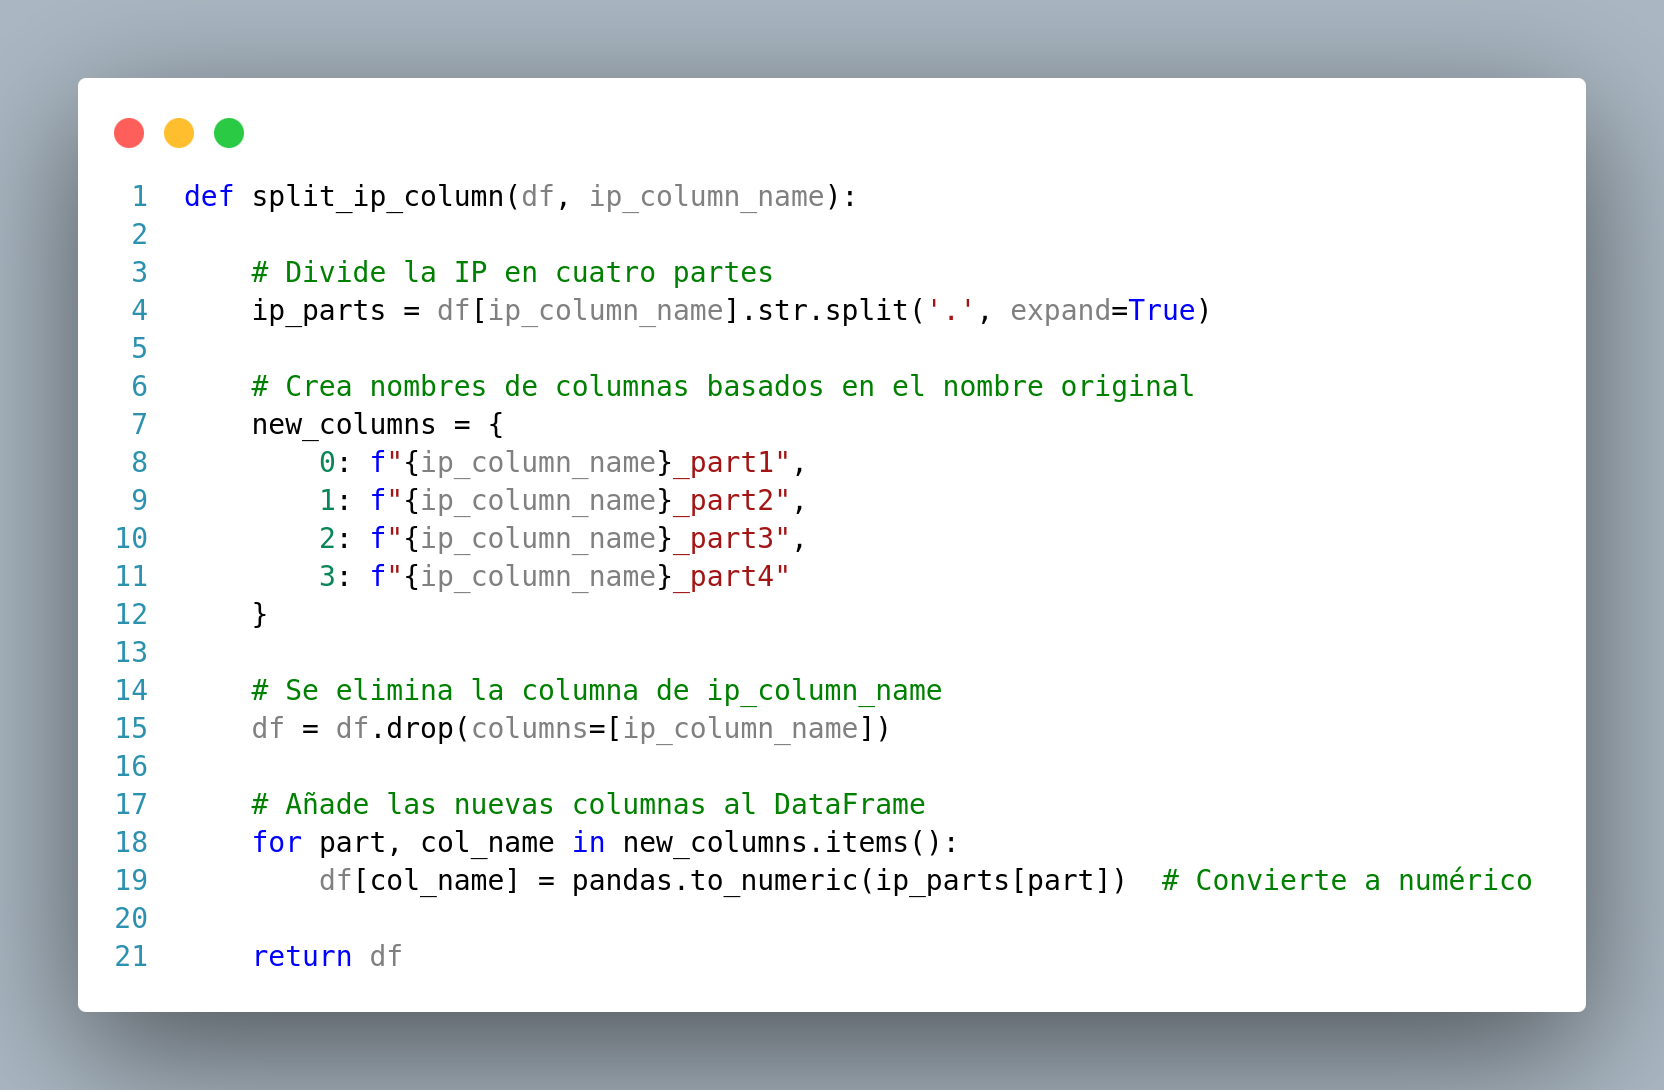
\includegraphics[width=0.8\textwidth]{./img/ent-datos/funIPv4.png}
    \caption{Función de transformación para los parámetros IPv4.}
    \label{fig:funIPv4}
\end{figure}

\end{itemize}

Una vez que todos los parámetros presentan valores numéricos, se separan los parámetros ente los que formarán parte de la entrada del modelo neuronal como atributos (a partir de ahora se les menciona como X) y los que contienen el valor de la salida que debe proporcionar el modelo neuronal llamados etiquetas(a partir de ahora se les menciona como Y).

Los parámetros que pertenecen a Y son \texttt{Label} y \texttt{Attack}. Sin embargo, en función del modelo que se entrena se utiliza o bien \texttt{Label}, o bien \texttt{Attack}, pero nunca los dos al mismo tiempo.

Por su parte, X la conforman el total de los parámetros del \textit{dataset} a excepción de:
\begin{itemize}
	\item \textbf{\texttt{Label} y \texttt{Attack}}: Se trata de los parámetros que conforman Y o etiquetas, si estos parámetros formasen parte de los datos de entrada del modelo, el algoritmo encargado de entrenarlo, les asignaría a estos parámetros unos pesos muy elevados y tendría una tasa teórica de éxito del 100\%, puesto que, se estaría introduciendo la respuesta al problema que se aborda directamente como entrada al modelo. En un sistema informático real esta práctica es imposible.
	\item \textbf{\texttt{IPV4\_SRC\_ADDR} y \texttt{IPV4\_DST\_ADDR}}: Tal y como se menciona en la sección \ref{sec.param-datos} \nameref{sec.param-datos}, estos parámetros presentan un patrón irregular y sintético. Al introducir estos parámetros como entradas para el entrenamiento del modelo, de forma análoga a como sucede con los parámetros \texttt{Label} y \texttt{Attack} se estarían introduciendo valores que no se pueden obtener en una situación realista y condicionando el comportamiento del modelo. Esto implica como se menciona en los siguiente capítulos que el modelo resultante obtendría muy buenas métricas en validación pero muy malas al someterlo a datos que nunca ha visto durante su entrenamiento.
	\item \textbf{\texttt{FLOW\_START\_MILLISECONDS} y \texttt{FLOW\_END\_MILLISECONDS}}: A diferencia de los anteriores parámetros, estos muestran valores que puedan condicionar el entrenamiento de los modelos ni sus resultados, pero se trata de parámetros que ofrecen información redundante, pues el parámetro \texttt{FLOW\_DURATION\_MILLISECONDS} es combinación lineal de estos dos. Al eliminar estos parámetros se agiliza el entrenamiento del modelo y su tiempo de respuesta una vez entrenado sin perjudicar su precisión.
\end{itemize}

Como el conjunto de datos original presentaba 53 atributos de entrada a los modelos y se ha descartado el uso de 4 de ellos, los modelos serán entrenados con 49 atributos de entrada. 

Para finalizar con el tratamiento de los datos, se normalizan los valores de X para que no haya tanta varianza entre los parámetros que lo conforman. Para normalizar los valores se utiliza el escalador \texttt{MinMaxScaler} que forma parte de la biblioteca \texttt{sklearn.preprocessing} junto con el método \texttt{fit\_transform} que se menciona en la explicación de la transformación del parámetro \texttt{Attack}. Llamando a \texttt{MinMaxScaler} con un rango (0,1), tras haber tratado los datos con el método \texttt{fit\_transform}, se obtienen valores escalados en un rango entre 0 y 1, lo que facilita la comparación y el procesamiento por parte de los algoritmos de aprendizaje automático sin alterar las relaciones proporcionales inherentes en los datos originales.


\chapter{Modelos}

\section{¿Qué es un modelo neuronal?}

En esta sección, se explica qué es un modelo neuronal, sus características y cómo funciona en el contexto de la inteligencia artificial. 

Los modelos neuronales son estructuras computacionales inspiradas en el cerebro humano, diseñadas para procesar información mediante una red de unidades interconectadas que imitan, de manera simplificada, la forma en que las neuronas biológicas se comunican entre sí cite{goodfellow2016deep}.

Los descurbrimientos del Premio Nobel de biología español, Santiago Ramón y Cajal sobre la estructura y funcionamiento de las neuronas, proporcionaron las bases para la comprensión del sistema nervioso en el que se basan los modelos de inteligencia artificial. A finales del siglo XIX, Cajal formuló la teoría de que las neuronas son células individuales conectadas por sinapsis, una idea que revolucionó la neurociencia y sirvió de inspiración para los modelos computacionales de redes neuronales. Su trabajo permitió comprender cómo las señales eléctricas viajan entre las neuronas y cómo se pueden formar conexiones adaptativas, conceptos que más tarde serían adoptados en el diseño de redes neuronales artificiales.

Un modelo neuronal es una arquitectura matemática que busca resolver problemas complejos de aprendizaje mediante el procesamiento de datos. Está compuesto por una serie de unidades de procesamiento, conocidas como neuronas artificiales, organizadas en capas. Cada capa recibe la salida de la capa anterior, aplica una función matemática sobre los datos y transmite el resultado a la siguiente capa. Este proceso se repite de manera secuencial hasta que se alcanza la capa de salida, que proporciona el resultado final del modelo \cite{bishop2006pattern}.

\begin{figure}[H]
    \centering
    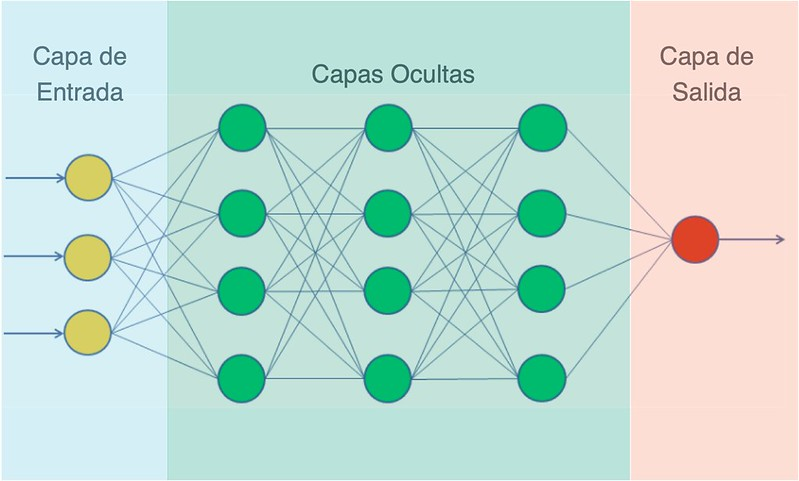
\includegraphics[width=0.8\textwidth]{./img/modelo/capas.png}
    \caption{Esquema de redes neuronales. \cite{aprendeia2021deep}}
    \label{fig:esq-capas}
\end{figure}

Las neuronas dentro de un modelo neuronal no operan de forma aislada, sino que están conectadas entre sí a través de enlaces denominados "pesos". Estos pesos determinan la importancia de la señal que se transmite de una neurona a otra. Durante el proceso de entrenamiento, los pesos se ajustan con el objetivo de minimizar el error en la salida del modelo, lo que permite que el modelo "aprenda" de los datos y mejore su capacidad para predecir o clasificar nueva información \cite{haykin2009neural}.

El proceso de entrenamiento de un modelo neuronal implica la retroalimentación o backpropagation, donde el error de la predicción se calcula y se distribuye hacia atrás a través de la red para ajustar los pesos de manera que el modelo se optimice progresivamente. En este sentido, el modelo neuronal tiene la capacidad de adaptarse a distintos tipos de datos y mejorar su rendimiento con el tiempo \cite{nielsen2015neural}.

A grandes rasgos, un modelo neuronal es una estructura computacional que imita el funcionamiento del cerebro humano para procesar y aprender de datos, y se utiliza en tareas como clasificación, predicción y reconocimiento de patrones.


\subsection{¿Qué tipos de modelos neuronales existen?}

En esta sección se explican cuales son tipos de modelos neuronales existen y sus características principales. 

Los modelos neuronales pueden clasificarse según su estructura, la forma en que procesan la información y la aplicación específica a la que están destinados. Estos modelos neuronales son fundamentales para resolver una variedad de problemas en áreas relacionadas con la inteligencia artificial como la visión por computadora, el procesamiento del lenguaje natural y el reconocimiento de patrones.

Uno de los tipos más comunes de modelos neuronales es el perceptrón multicapa (MLP), que está formado por varias capas de neuronas organizadas en una estructura jerárquica. Cada capa en un MLP recibe la salida de la capa anterior y la procesa mediante una función de activación antes de pasar el resultado a la siguiente capa. Este tipo de red se utiliza principalmente para tareas de clasificación y regresión, y su entrenamiento se realiza utilizando algoritmos como el de retropropagación. Es el tipo de modelo que se utiliza en este proyecto para obtener un modelo capaz de detectar instrusiones en una red informática. \cite{goodfellow2016deep}

Otro tipo importante de modelo neuronal es la red neuronal convolucional (CNN), que está diseñada específicamente para procesar datos con una estructura de cuadricula, como las imágenes. En una CNN, las neuronas están organizadas en capas convolucionales que aplican filtros a los datos de entrada para extraer características relevantes, como bordes, texturas o formas. Esta estructura permite que las CNN sean altamente eficaces para tareas como el reconocimiento de imágenes y la visión por computadora \cite{goodfellow2016deep}.


\begin{figure}[H]
    \centering
    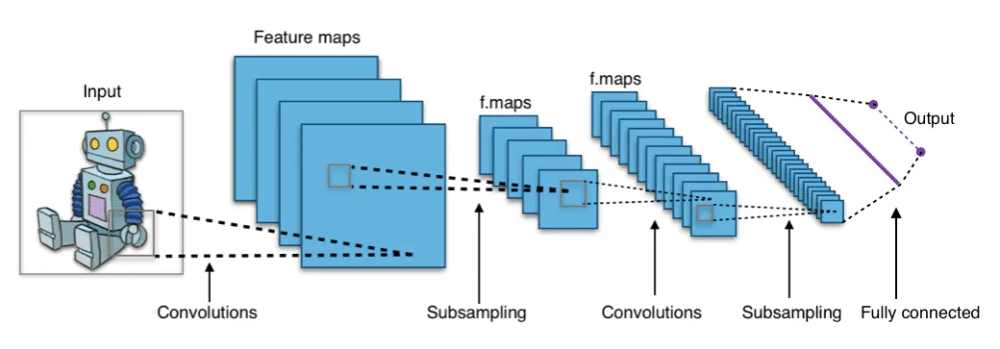
\includegraphics[width=0.8\textwidth]{./img/modelo/CNN.png}
    \caption{Esquema de redes neuronal convolucional. \cite{uniteai2020cnn}}
    \label{fig:esq-CNN}
\end{figure}


Las redes neuronales recurrentes (RNN), por otro lado, son adecuadas para procesar secuencias de datos, como el texto o el audio. Las RNN son únicas porque sus neuronas tienen conexiones que permiten que la información fluya hacia atrás a lo largo del tiempo, lo que las hace útiles para modelar dependencias temporales en los datos. Este tipo de red es comúnmente utilizado en tareas de procesamiento de lenguaje natural y en modelos de predicción de series temporales \cite{haykin2009neural}.

En un enfoque más avanzado, existen las redes generativas antagónicas (GAN), que se componen de dos redes neuronales: un generador y un discriminador. El generador crea datos falsos a partir de ruido, mientras que el discriminador intenta diferenciar entre los datos reales y los generados. A través de un proceso de entrenamiento competitivo, ambas redes mejoran en sus respectivas tareas. Las GANs se utilizan principalmente en la generación de imágenes, música y otros tipos de contenido artístico \cite{nielsen2015neural}.

\subsection{Función de perdida}
En esta sección se explica que es una función de pérdida y su importancia en el proceso de entrenamiento de un modelo neuronal. También se justifica el uso de las funciones de pérdida que se emplean para el entrenamiento de los modelos de este trabajo.

Una función de pérdida es un componente fundamental en el entrenamiento de modelos de aprendizaje automático, cuya finalidad consiste en cuantificar la discrepancia entre las predicciones generadas por el modelo y los valores reales esperados. Esta medida permite guiar el proceso de optimización, ya que el objetivo durante el entrenamiento es minimizar dicha pérdida para mejorar la precisión del modelo.\cite{eitca_loss_function}

Las funciones de pérdida desempeñan un papel central en la formulación matemática del aprendizaje supervisado, al establecer una métrica que penaliza el error cometido por el modelo. Esta penalización permite que los algoritmos de optimización, como el descenso por gradiente, ajusten iterativamente los parámetros del modelo en la dirección que reduce la pérdida total. Para que esta estrategia sea efectiva, la función de pérdida debe poseer ciertas propiedades fundamentales:

\begin{itemize}

    \item\textbf{Diferenciabilidad}: Permite el cálculo de gradientes necesarios para optimizar los parámetros mediante técnicas basadas en derivadas, como el descenso por gradiente.

    \item\textbf{Convexidad (deseable)}: Favorece la convergencia hacia un mínimo global, aunque en la práctica, muchos modelos no lineales presentan funciones de pérdida no convexas.

    \item\textbf{Estabilidad numérica}: Previene errores computacionales al manejar valores extremos o transformaciones exponenciales, manteniendo precisión durante el entrenamiento.

 	\item\textbf{Sensibilidad al error}: Garantiza que los errores mayores se penalicen de forma más significativa, orientando el modelo hacia mejores predicciones.

	\item\textbf{Escalabilidad}: Permite su aplicación eficiente en contextos con grandes volúmenes de datos y arquitecturas de red complejas.

\end{itemize}

Estas propiedades aseguran que la función de pérdida cumpla su objetivo central, actuar como un mecanismo confiable y eficiente para guiar la actualización de los parámetros del modelo. \cite{ultralytics_loss_function}

En el caso específico del modelo de clasificación binaria, se opta por la función BCEWithLogitsLoss (Binary Cross Entropy with Logits Loss), que está especialmente recomendada para utilizarse en entornos de aprendizaje profundo como PyTorch, entorno utilizado en el desarrollo práctico de este proyecto. Esta función combina en una sola operación dos pasos fundamentales: la aplicación de la función sigmoide y el cálculo de la entropía cruzada binaria. Al integrar ambos procedimientos en una única función, se obtienen varias ventajas prácticas.\cite{datacamp_loss_function}

En primer lugar, se mejora la estabilidad numérica, ya que evita operaciones redundantes que podrían dar lugar a pérdidas de precisión, especialmente al manejar las salidas no normalizadas del modelo (logits) con valores extremos.

En segundo lugar, se optimiza el rendimiento computacional, al reducir el número de transformaciones necesarias antes del cálculo de la pérdida. 

Finalmente, permite trabajar directamente con logits, lo cual simplifica la implementación y reduce errores potenciales derivados de transformaciones incorrectas. \cite{bigdatafran_pytorch_classification}




\subsection{Algoritmo de optimización}\label{sec:alg-opt}
En esta sección se explica qué es un algoritmos de optimización,su funcionamiento, sus principales características, su importancia dentro del proceso de entrenamiento de modelos neuronales y algunos ejemplo de los algoritmos de optimización más utilizados.

Un algoritmo de optimización es un conjunto de procedimientos matemáticos y computacionales cuyo propósito es encontrar el mejor valor posible (o el más cercano a este) para un conjunto de parámetros o variables dentro de un problema específico. Estos algoritmos buscan minimizar o maximizar una función objetivo, que representa el rendimiento del sistema o modelo a optimizar. En el contexto de entrenamiento de redes neuronales, la función objetivo comúnmente se refiere a una función de pérdida, que cuantifica la diferencia entre las predicciones del modelo y las etiquetas reales de los datos. Los algoritmos de optimización ajustan los parámetros (pesos y sesgos) de la red neuronal durante el proceso de entrenamiento con el fin de reducir dicha diferencia \cite{goodfellow2016deep}.


El funcionamiento de un algoritmo de optimización se basa en un proceso iterativo en el que se ajustan los parámetros de la red neuronal utilizando información acerca del gradiente de la función de pérdida con respecto a estos parámetros. En este contexto, la retropropagación juega un papel crucial, ya que es el método utilizado para calcular esos gradientes. A través de la retropropagación, el error de la red se propaga hacia atrás desde la capa de salida hasta las capas anteriores, permitiendo calcular cómo cada parámetro contribuye al error total. Posteriormente, el algoritmo de optimización utiliza estos gradientes calculados por la retropropagación para actualizar los parámetros de la red en la dirección opuesta al gradiente, con el objetivo de reducir progresivamente la pérdida. Generalmente, se utilizan técnicas de descenso de gradiente para realizar estos ajustes. Durante cada iteración, el algoritmo calcula el gradiente de la función de pérdida a través de la retropropagación y lo utiliza para modificar los parámetros de manera eficiente, buscando alcanzar el mínimo global o local de la función de pérdida \cite{bottou2010large}.

\begin{figure}[H]
    \centering
    \includegraphics[width=0.8\textwidth]{./img/modelo/retropropagacion.png}
    \caption{Esquema de algoritmo de optimización usando los gradiente calculados por la retropropagación. \cite{msmk2023backpropagation}}
    \label{fig:esq-Optimizacion}
\end{figure}



Las características clave de los algoritmos de optimización incluyen la tasa de aprendizaje, la capacidad para escapar de mínimos locales, y la convergencia en un tiempo razonable. La tasa de aprendizaje (learning rate o lr) es un hiperparámetro crítico que determina la magnitud de los ajustes que se realizan en los parámetros del modelo durante cada iteración. Si el learning rate es muy alto, el algoritmo puede saltar el mínimo global, por otro lado, si es muy baja, el proceso puede volverse muy lento. Los métodos de optimización varían en cuanto a la forma en que gestionan estas características, algunos métodos mejoran la eficiencia utilizando técnicas como el momento, la normalización del gradiente, o el uso de segunda orden \cite{kingma2014adam}.


La importancia de los algoritmos de optimización en el entrenamiento de redes neuronales es fundamental, ya que la capacidad de un modelo para aprender de los datos y generalizar de manera efectiva depende en gran medida de cómo se optimizan los parámetros de la red. Un algoritmo de optimización bien elegido y configurado puede significar la diferencia entre un modelo con un rendimiento subóptimo y uno que logra altos niveles de precisión y eficiencia. De esta manera, la correcta selección y ajuste de estos algoritmos se considera un aspecto crucial para el desarrollo exitoso de modelos de aprendizaje profundo y redes neuronales \cite{goodfellow2016deep}.

Existen varios algoritmos de optimización ampliamente utilizados en el entrenamiento de redes neuronales. Entre los más comunes se encuentran el Descenso de Gradiente Estocástico (SGD), Momentum, Adagrad, RMSprop y Adam. El SGD es uno de los más simples y fundacionales, pero sufre de inestabilidad debido a su naturaleza estocástica y la falta de adaptación de la tasa de aprendizaje. Momentum ayuda a mejorar la convergencia al incorporar la información de los gradientes pasados, lo que permite que el modelo escape de los mínimos locales más fácilmente. Adagrad adapta la tasa de aprendizaje para cada parámetro, mientras que RMSprop ajusta la tasa de aprendizaje utilizando una media móvil del gradiente, lo que mejora la estabilidad \cite{bottou2010large}.

Sin embargo, el algoritmo más recomendado para entrenar un modelo de clasificación binaria es Adam (Adaptive Moment Estimation). Adam combina las ventajas del descenso de gradiente estocástico y el momento, adaptando la tasa de aprendizaje de manera eficiente para cada parámetro del modelo. Esto lo hace particularmente adecuado para tareas de clasificación binaria, ya que garantiza una convergencia más rápida y estable, minimizando el riesgo de sobreajuste (overfitting) mientras se optimizan los parámetros del modelo. Sin embargo, una variante reciente de Adam, conocida como AdamW, introduce un cambio importante en la forma en que se maneja la regularización de los parámetros. AdamW separa explícitamente la actualización de los pesos y la regularización (típicamente L2 o weight decay), lo que mejora la eficacia de la regularización sin interferir con la adaptación de la tasa de aprendizaje.

Aunque ambos algoritmos, Adam y AdamW, tienen un rendimiento destacado en tareas de clasificación binaria, AdamW se ha demostrado más eficaz en la prevención de sobreajuste en redes neuronales complejas. Esto se debe a su tratamiento explícito del weight decay, lo que permite una mejor generalización en problemas con grandes volúmenes de datos como el que se trata en este proyecto. Sin embargo, Adam sigue siendo una opción popular y efectiva, especialmente cuando se trabaja con redes neuronales menos complejas o cuando se desea una mayor estabilidad y rapidez de convergencia. En general, AdamW es preferido en situaciones donde la regularización adecuada es crucial, pero Adam sigue siendo una opción sólida y eficiente. \cite{kingma2014adam}.


\section{Parámetros e hiperparámetros}\label{sec:paramhiper}
En este apartado se explica que son los parámetros y los hiperparámetros de un modelo neurnal. También se listan y describen los principales hiperparámetros que se deben de tener en cuenta al entrenar un modelo neuronal. 

Los parámetros de un modelo neuronal son los valores ajustables que el modelo aprende a partir de los datos durante el proceso de entrenamiento. Estos parámetros incluyen los pesos y sesgos de las conexiones entre las neuronas de las diferentes capas de la red neuronal. Los pesos determinan la importancia de las entradas de cada neurona, mientras que los sesgos permiten ajustar la salida de cada neurona antes de la activación. Como se explica en los apartado anteriores, el aprendizaje de estos parámetros se realiza mediante algoritmos de optimización como el gradiente descendente, los cuales buscan minimizar la función de pérdida. \cite{goodfellow2016deep}


Los hiperparámetros son los valores que se configuran antes del entrenamiento y no se ajustan directamente durante el proceso de aprendizaje. Este tipo de parámetros controlan el comportamiento del proceso de entrenamiento y afectan la capacidad del modelo para aprender patrones complejos de los datos. A diferencia de los parámetros, los hiperparámetros deben ser establecidos manualmente o mediante técnicas de optimización específicas, como la búsqueda en cuadrícula o la búsqueda aleatoria, técnicas que se aplcian en las siguientes secciones de este documento. Los hiperparámetros influyen en aspectos clave como la velocidad de aprendizaje, la regularización y la estructura de la red \cite{chollet2018deep}. Los más importantes son:

\begin{itemize}

    \item \textbf{Tasa de aprendizaje (Learning rate)}: Controla la magnitud de los ajustes realizados en los pesos durante cada iteración del entrenamiento. Como se comenta en \ref{sec:alg-opt} \nameref{sec:alg-opt}, una tasa demasiado alta puede hacer que el modelo no converja, mientras que una tasa demasiado baja puede llevar a una convergencia muy lenta.
    
    \item \textbf{Número de épocas (Epochs)}: El número de épocas se refiere a cuántas veces el algoritmo de entrenamiento recorre todo el conjunto de datos. Un número adecuado de épocas permite que el modelo aprenda de manera efectiva, sin embargo, demasiadas épocas pueden llevar al sobreajuste.
    
    \item \textbf{Tamaño del lote (Batch size)}: El tamaño del lote determina la cantidad de ejemplos utilizados en cada actualización de los pesos. Un tamaño de lote pequeño puede hacer que el modelo sea más ruidoso y difícil de entrenar, mientras que un tamaño de lote grande puede hacer que el entrenamiento sea más estable, pero menos eficiente.
    
    \item \textbf{Número de capas ocultas (Hidden layers)}: Este hiperparámetro define la profundidad de la red neuronal, es decir, el número de capas intermedias entre la capa de entrada y la capa de salida. Un mayor número de capas permite modelar funciones más complejas, pero también aumenta el riesgo de sobreajuste.
    
    \item \textbf{Número de neuronas por capa (Hidden factor)}: Este parámetro establece la cantidad de neuronas en cada capa oculta. Un mayor número de neuronas puede mejorar la capacidad del modelo para capturar patrones complejos, aunque también aumenta el tiempo de entrenamiento y la complejidad computacional.
\end{itemize}



\section{Modelo neuronal de clasificación binaria} \label{sec.modBIN}
En esta sección se describe tanto el proposito como los procedimientos empleados para el desarrollo del modelo de clasificación binaria. Se detalla el proceso de selección de hiperparámetros, así como las distintas arquitecturas diseñadas con el fin de identificar la combinación que optimiza el rendimiento del modelo. Además, se presenta una comparación entre las arquitecturas evaluadas para determinar la más adecuada.

%Finalmente, se especifican las métricas utilizadas para la evaluación y selección de las mejores combinaciones de hiperparámetros.

\subsection{Proposito del modelo de clasificación binaria}
El modelo de clasificación binaria se ha diseñado con el objetivo de identificar de manera precisa y eficiente, si una instancia de tráfico de red corresponde a una actividad legítima o a un comportamiento malicioso. Su función principal consiste en distinguir entre accesos normales y posibles intentos de intrusión, permitiendo así la detección temprana de ataques y contribuyendo a la protección proactiva de los sistemas informáticos.

\subsection{Diseño del modelo e hiperparámetros seleccionados} \label{sec:disBIN}
En esta sección se detalla cual es el diseño del modelo de clasificación binaria escogido, así como los valore de los hiperparámetros utilizados durante los experimentos en el entrenamiento del modelo y sus correspondientes justificaciones.

Para diseñar la arquitectura del modelo, se ha desarrollado la clase Modelo. Esta clase está conformada por dos funciones, la primera corresponde con la inicialización de la clase, y la segunda con la arquitectura utilizada para este modelo.

Como se puede observar en la figura \ref{fig:modBIN}, el modelo está compuesto por dos capas. La capa1 tiene un número de entradas igual al número de parámetros que poseen los datos utilizados para entrenar al modelo y un número de salidas que depende del parámetro \textit{ventaOculta}, con el que se llama a la función de inicialización del modelo. El número de salidas de la capa1 será precisamente el que determine la arquitectura específica que se utiliza. Por su parte, la capa2 recibe como entrada el número de salidas de la capa1 y al tratarse de la capa final de un modelo de clasificación binaria, esta capa tendrá una única salida.

Debido a que la función de pérdida utilizada para entrenar el modelo es BCEWithLogitsLoss(), que ya aplica la función sigmoidea, sería contraproducente aplicar la función sigmoidea sobre la salida del modelo para su entrenamiento.


\begin{figure}[H]
    \centering
    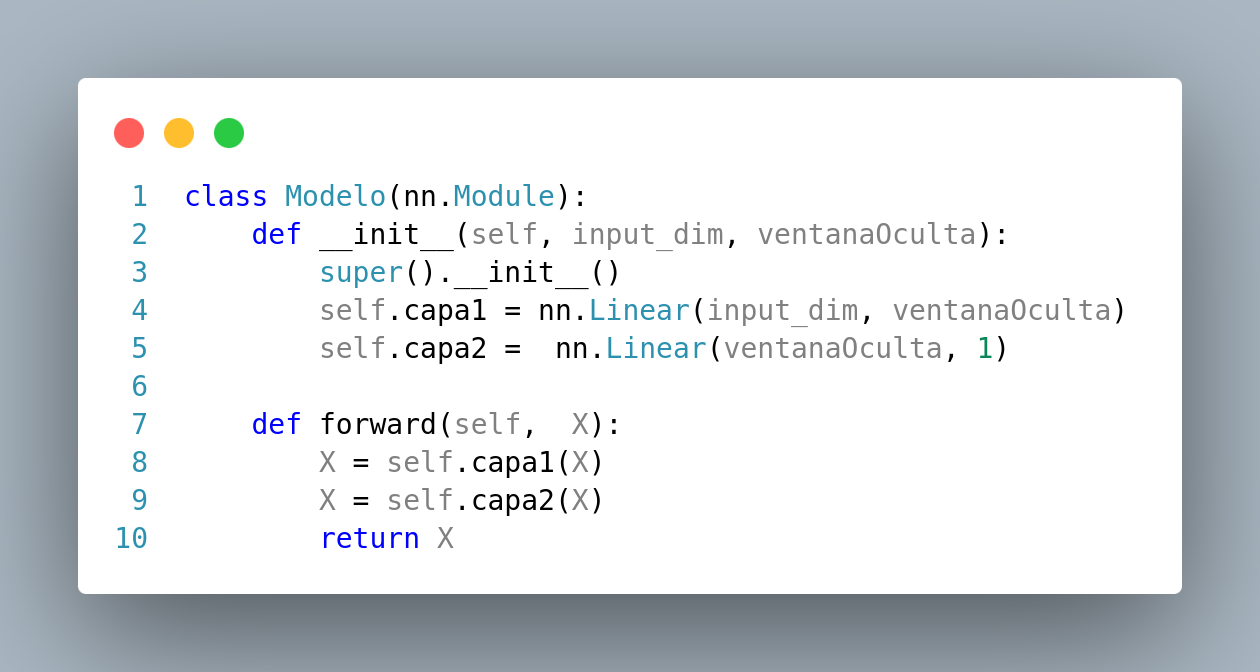
\includegraphics[width=0.8\textwidth]{./img/modelo/modeloBIN.png}
    \caption{Estructura del modelo de clasificación binaria diseñada.}
    \label{fig:modBIN}
\end{figure}

Para evitar el sobreajuste del modelo y obtener valores de las predicciones más confiables que se utilizarán para la evaluación del rendimiento del modelo, se utiliza validación cruzada k-fold. La validación cruzada consiste en dividir los datos de entrenamiento en n folds que se utilizan para entrenar al modelo con n-1 folds y después validar el modelo entrenado con el fold que no se ha utilizado para entrenarlo. Este proceso se repite para los n folds y en cada iteración es un fold distinto el que no se utiliza para el entrenamiento. Una vez completadas las iteraciones se extraen las medias de las métricas obtenidas con cada fold durante la validación. Para entrenar el modelo de clasificación binaria, se ha utilizado StratifiedKFold() que como su nombre indica, estratifica los folds para que las proporciones de las clases de los datos utilizados para el entrenamiento se mantengan similares en cada fold y no se creen folds con un único tipo de clase. Estratificar los datos es especialmente crítico para aquellos datasets cuyos datos están muy desbalanceados como es el caso de los datos utilizados para entrenar los modelos de este proyecto. Para el entrenamiento del modelo de clasificación binaria, se ha optado por utilizar validación cruzada StratifiedKFold con 5 folds o divisiones.

Como algoritmo de optimización para el entrenamiento del modelo de clasificación binaria, se ha optado por utilizar AdamW(). Como se comenta en la sección \ref{sec:alg-opt} \nameref{sec:alg-opt}, se ha demostrado que AdamW es más eficaz en la prevención de sobreajuste en redes neuronales que otros algoritmos de optimización. Además, permite una mejor generalización en problemas con grandes volúmenes de datos como el que se trata en este proyecto.

Los hiperparámetros que han sido seleccionados para encontrar la mejor configuración para el modelo de clasificación binaria diseñado son: el batch size, la tasa de aprendizaje (learning rate) y el número de épocas. Estos hiperparámetros resultan imprescindibles en el entrenamiento de modelos de clasificación binaria, dado que influyen directamente en la eficiencia del proceso de optimización y en la calidad del modelo resultante.

Como se comenta en la sección \ref{sec:paramhiper} \refname{sec:paramhiper}, los hiperparámetros controlan el comportamiento del proceso de entrenamiento y afectan la capacidad del modelo para aprender patrones complejos de los datos. Teniendo en cuenta las características de cada hiperparámetro, se han escogido los siguientes valores para los experimentos del entrenamiento del modelo binario con el objetivo de encontrar la mejor combinación de ellos.

\begin{itemize}
	\item \textbf{Batch size}: Teniendo en cuenta el tamaño de los datos que se utilizan para la fase de entrenamiento del modelo binario, se han considerado que los valores [2000, 10000, 15000, 20000], eran apropiados y suficientemente dispares como para notar diferencias significativas en los resultados de la ejecución de los experimentos.
	\item \textbf{Learning rate}: Siguiendo los avisos de la sección anterior en la que se explicaba el propósito y características de cada hiperparámetro, se ha optado por elegir unos valores con los que se espera que el modelo converja sin sobreajustarse ni se exceda en el tiempo de obtención de una solución válida. Los valores elegidos han sido [0.01, 0.001, 0.0001].
	\item \textbf{Épocas}: De forma similar a como sucede con la tase de aprendizaje, un valor excesivamente bajo en el número de épocas puede provocar que el modelo no converja. Sin embargo, un número demasiado alto de épocas provoca sobreajuste en el modelo. Teniendo en cuenta las consideraciones mencionadas, los valores que se han probado para este hiperparámetro son [10, 20, 30].
\end{itemize}

\subsection{Arquitecturas desarrolladas}
En esta sección se abordan cuales son las arquitecturas a desarrollar para el modelo de clasificación binaria. Como se comenta en la sección anterior \ref{sec:disBIN} \nameref{sec:disBIN}, la diferencia entre las arquitecturas radica en el tamaño de la capa oculta del modelo.

Para el desarrollo de las diferentes arquitecturas, se ha optado por realizar experimentos de entrenamiento del modelo de clasificación binaria con un tamaño de ventana oculta igual a:
la mitad del número de parámetros que recibe el modelo, el mismo número que parámetros que tiene el modelo y doble del número de parámetros. Esto equivale a un tamaño de la capa de venta oculta de 25, 49 y 98 respectivamente. Estos valores se obtienen de forma dinámica después de tratar los datos del csv  utilizado para los entrenamientos y las pruebas de este proyecto.

A continuación, se comentan las posibles ventajas e inconvenientes de cada arquitectura que se esperan antes de realizar los experimentos.

\subsubsection{Capa oculta con la mitad de neuronas que parámetros de entrada}\label{sec:VIBIN25}
En este apartado se comentan cuales son las principales ventajas e inconvenientes, a priori, de un modelo de clasificación binaria con un número de neuronas en la capa oculta igual a la mitad del número de parámetros que recibe el modelo.

\paragraph{Ventajas (n/2)}
\begin{itemize}
	\item El riesgo de sobreajuste es menor, esto es especialmente importante si no se utiliza validación cruzada o el conjunto de datos de entrenamiento es pequeño o simple.
	\item  Al tener un número de neuronas menor, tanto la función  de pérdida como el algoritmo de optimización, tardan menos en realizar los cálculos de los ajustes de los pesos y sesgos del modelo. Este menor coste de cálculo se refleja directamente en el tiempo necesario para entrenar el modelo y en el tiempo de respuesta del mismo una vez entrenado.
	\item Un número bajo de neuronas es especialmente útil cuando los datos son linealmente separables o poco complejos.
\end{itemize}
\paragraph{Inconvenientes(n/2)}
\begin{itemize}
	\item Si las relaciones entre los datos son demasiado complejas, el moelo puede sufrir underfitting o subajuste.
	\item Sensibilidad alta a la inicialización de los pesos, lo que puede provocar que un porcentaje alto de neuronas no se utilicen por tener pesos iguales o muy cercanos a 0. Esto implica que parte de la capacidad de la red quede inutilizada, empeorando el rendimiento incluso en problemas simples.
\end{itemize}

Tras comentar cuales son las principales ventajas e inconvenientes de utilizar una capa oculta con un número de neuronas igual a la mitad de los parámetros del modelo, aparentemente, las propiedades del conjunto de datos que se utiliza para entrenar al modelo no son las idóneas para esta arquitectura y no se esperan resultados especialmente destacables.

\subsubsection{Capa oculta con el mismo número de neuronas que parámetros de entrada}\label{sec:VIBIN49}
En este apartado se comentan cuales son las principales ventajas e inconvenientes, a priori, de un modelo de clasificación binaria con un número de neuronas en la capa oculta igual al número de parámetros que recibe el modelo.

\paragraph{Ventajas (n)}
\begin{itemize}
	\item La capacidad y la generalización están balanceadas, esto significa que el modelo evita tanto el sobreajuste como el subajuste.
	\item Es capaz de modelar relaciones más complejas entre conjuntos de datos que arquitecturas con un número de neuronas menor, lo que es especialmente útil en problemas con relaciones no lineales` entre sus datos.
	\item Son computacionalemnte más eficientes que arquitecturas con un número elevado de neuronas en la capa oculta. 
\end{itemize}
\paragraph{Inconvenientes(n)}
\begin{itemize}
	\item Puede resultar insuficiente en problemas demasiado complejos o con un gran volumen de datos.
	\item Si el conjunto de datos utilizado para entrenar el modelo es pequeño puede sobreajustar.
\end{itemize}

Tras comentar cuales son las principales ventajas e inconvenientes de utilizar una capa oculta con el mismo número de neuronas que parámetros recibe el modelo, aparentemente, esta arquitectura ofrecera resultados significativamente positivos gracias a su equilibrio y balanceo.

\subsubsection{Capa oculta con el doble de neuronas que parámetros de entrada}\label{sec:VIBIN98}
En este apartado se comentan cuales son las principales ventajas e inconvenientes, a priori, de un modelo de clasificación binaria con el doble de neuronas en la capa oculta que parámetros recibe el modelo.

\paragraph{Ventajas (n*2)}
\begin{itemize}
	\item Alta capacidad de aprendizaje, lo que se traduce como la posibilidad de capturar patrones de datos muy complejos que no son lineales ni perceptibles en un análisis superficial del problema.
	\item Cuanto mayor es el conjunto de datos mejor se ajustan los pesos.
	\item Es menos propenso a subajustar que otras arquitecutras.
\end{itemize}
\paragraph{Inconvenientes(n*2)}
\begin{itemize}
	\item El riesgo de sobreajuste es elevado, memorizando de esta manera ruido en vez de aprender los patrones generalizables.
	\item Nivel computacional muy elevado, lo que se refleja en el tiempo necesario de entrenamiento de esta arquitectura y en su posterior tiempo de respuesta.
	\item Si el número de muestras del conjunto de datos es bajo tiende a sobreajustar.
\end{itemize}

Tras comentar cuales son las principales ventajas e inconvenientes de utilizar una capa oculta con un número de neuronas igual al doble de los parámetros del modelo, aparentemente, esta arquitectura obtendrá mejores resultados si los parámetros no tiene relaciones lineales. En cambio, si los datos presentan relaciones lineales tiene más probabilidades de sobreajustar los pesso del modelo, lo que implicaría que le modelo no ha sido capaz de converger a una solución genérica.

\section{CREAR E INSERTAR IMAGENES DE LAS ARQUITECTURAS}


\subsection{Matriz de confusión para clasificación binaria} \label{sec.matriz-consfusion}
En esta sección se explica en que consiste una matriz de confusión y las variaciones que existen de las matrices de confusión en función del tipo de modelo neuronal de clasificación que se entrene. Son una herramienta fundamental utilizada en el campo del aprendizaje automático y la clasificación, especialmente cuando se evalúan modelos de clasificación como el que se propone en este proyecto.

La matriz de confusión es una representación tabular que permite evaluar el rendimiento de un modelo de clasificación. Esta matriz compara las predicciones del modelo con los valores reales (verdaderos) y proporciona una visión detallada sobre los errores cometidos. Esta matriz permite calcular diversas métricas de evaluación del modelo, que son esenciales para entender la efectividad del modelo en tareas de clasificación.

En el caso de los modelos neuronales de clasificación binaria, la matriz tiene una estructura 2x2, donde cada celda en la matriz representa la cantidad de veces que una combinación específica de clase real y clase predicha ocurrió. Los valores posibles para la clasificación binaria son: 

\begin{itemize}

	\item Verdaderos positivos (VP): son las instancias que pertenecen a la clase positiva y que el modelo ha clasificado correctamente como positivas.

    \item Falsos positivos (FP): corresponden a las instancias que no pertenecen a la clase positiva, pero que el modelo ha etiquetado incorrectamente como positivas.

    \item Falsos negativos (FN): se refieren a las instancias que deberían ser clasificadas como positivas, pero que el modelo ha predicho como negativas.

    \item Verdaderos negativos (VN): son las instancias que pertenecen a la clase negativa y que el modelo ha clasificado correctamente como negativas.

\end{itemize}



\begin{table}[h]
\centering
\label{tab:confusion_matrix}
\begin{tabular}{|l|c|c|}
\hline
 & \textbf{Predicción Positiva} & \textbf{Predicción Negativa} \\ \hline
\textbf{Real Positivo} & Verdaderos Positivos (VP) & Falsos Negativos (FN) \\ \hline
\textbf{Real Negativo} & Falsos Positivos (FP) & Verdaderos Negativos (VN) \\ \hline
\end{tabular}
\caption{Matriz de confusión para clasificación binaria.}
\end{table}

\subsection{Métricas útiles en clasificación binaria}  \label{sec.metricas-bin}
En esta sección se define el concepto de métrica, se explica cual es su importancia en el proceso de obtención de un modelo neuronal bien entrenado y se enumeran las métricas que se utilizan pàra el estudio del modelo de clasificación binaria desarrollado en este proyecto explicando la importancia de cada una de ellas.

Las métricas en el contexto de los modelos de aprendizaje automático son herramientas cuantitativas utilizadas para evaluar el rendimiento de un modelo entrenado. Estas métricas permiten medir si el modelo está realizando la tarea para la cual fue diseñado de manera correcta, comparando sus predicciones con los valores reales de los datos de prueba. Son fundamentales para comprender la efectividad del modelo y para identificar áreas de mejora, ya que proporcionan una evaluación objetiva y reproducible del comportamiento del modelo.

El uso adecuado de las métricas es crucial, ya que guían las decisiones sobre el ajuste y la optimización del modelo. Sin métricas claras, el proceso de evaluación se vuelve subjetivo y difícil de manejar. Además, las métricas permiten realizar comparaciones entre diferentes modelos o configuraciones, facilitando la selección del modelo más adecuado para una tarea específica. Una interpretación correcta de las métricas ayuda a evitar problemas como el sobreajuste o el subajuste, y garantiza que el modelo generalice bien a nuevos datos \cite{goodfellow2016deep}.

Para evaluar el desempeño del modelo de detección y clasificación de ataques, se utilizan las siguientes métricas derivadas de la matriz de confusión.


\begin{itemize}
    \item \textbf{Exactitud (\textit{Accuracy})}: \label{met:Accuracy}
    
\begin{equation}
    \text{Accuracy} = \frac{VP + VN}{VP + FP + VN + FN}
\end{equation}

En el entrenamiento de modelos neuronales para la detección de intrusiones, esta métrica representa la proporción del total de las clasificaciones realizadas correctamente. Indica la capacidad general del modelo para distinguir entre tráfico normal e intrusivo. Si bien ofrece una visión global del rendimiento, su valor disminuye en escenarios donde la cantidad de tráfico normal supera significativamente al tráfico malicioso, ya que el modelo puede obtener una alta exactitud simplemente clasificando la mayoría de las instancias como normales.

\item \textbf{Precisión (\textit{Precision})}: \label{met:Precision}

\begin{equation}
    \text{Precision} = \frac{VP}{VP + FP}
\end{equation}

Esta métrica evalúa la capacidad del modelo neuronal para evitar la identificación incorrecta de tráfico normal como intrusivo. En la detección de intrusiones, una alta precisión es crucial para minimizar las falsas alarmas, las cuales pueden generar una sobrecarga operativa en los equipos de seguridad, requiriendo la revisión de eventos benignos y distrayendo la atención de amenazas reales. Un modelo preciso reduce la fatiga de alertas y permite una respuesta más eficiente a incidentes genuinos.

\item \textbf{Sensibilidad (\textit{Recall})}: \label{met:Recall}

\begin{equation}
    \text{Recall} = \frac{VP}{VP + FN}
\end{equation}

La sensibilidad mide la habilidad del modelo neuronal para detectar todas las instancias de intrusión presentes en el tráfico de red. En el contexto de la seguridad, un alto recall es de suma importancia, ya que implica una menor probabilidad de que ataques reales pasen desapercibidos. Un modelo con baja sensibilidad puede tener consecuencias graves, permitiendo que actividades maliciosas se infiltren y comprometan la integridad y la confidencialidad de los sistemas.

\item \textbf{Puntuación F1 (\textit{F1-Score})}: \label{met:F1-score}

\begin{equation}
    F1 = 2 \times \frac{\text{Precision} \times \text{Recall}}{\text{Precision} + \text{Recall}}
\end{equation}

Esta métrica proporciona una evaluación equilibrada del rendimiento del modelo neuronal al calcular la media armónica entre la precisión y el recall. En la detección de intrusiones, donde a menudo existe un desequilibrio entre el tráfico normal y el malicioso, el F1-score ofrece una métrica más robusta que la exactitud, ya que considera tanto la capacidad de evitar falsas alarmas como la de detectar todas las intrusiones. Un valor alto de F1-score indica un buen compromiso entre ambas capacidades.

\item \textbf{Puntuación F2 (\textit{F2-Score})}: \label{met:F2-score}

\begin{equation}
    F2 = 5 \times \frac{\text{Precision} \times \text{Recall}}{4 \times \text{Precision} + \text{Recall}}
\end{equation}

Esta variante de la puntuación F pondera la sensibilidad más que la precisión. En el ámbito de la detección de intrusiones, el F2-score resulta útil cuando las consecuencias de no detectar un ataque (falso negativo) se consideran significativamente más perjudiciales que generar una falsa alarma (falso positivo). Al asignar un mayor peso al recall, se prioriza la identificación de la mayor cantidad posible de actividades maliciosas, incluso a expensas de un posible aumento en las falsas alertas.


\item \textbf{Área bajo la curva (\textit{ROC AUC})}: \label{met:ROCAUC}
\begin{equation}
    \text{FPR} = \frac{FP}{FP + VN}
\end{equation}
\begin{equation}
    \text{Recall}(\text{FPR}(t)) = \text{Recall}(t)
\end{equation}
\begin{equation}
    \text{ROC AUC} = \int_{0}^{1} \text{Recall}(\text{FPR}) \, d(\text{FPR})
\end{equation}



El área bajo la curva ROC (Receiver Operating Characteristic) mide la capacidad del modelo neuronal para discriminar entre clases positivas y negativas a lo largo de todos los posibles umbrales de decisión. 
En la curva ROC, la FPR (False Positive Rate) actúa como la variable del eje x, mientras que el Recall (o TPR, True Positive Rate) corresponde a la variable del eje y. En el contexto de la seguridad, un alto valor de AUC indica que el modelo asigna puntuaciones más altas a las intrusiones que al tráfico normal de manera consistente, lo que sugiere una buena capacidad de priorización de amenazas. Esta métrica es especialmente útil cuando se desea evaluar el rendimiento global del modelo sin depender de un umbral fijo. Un modelo con bajo AUC podría fallar al separar el tráfico malicioso, lo que aumentaría la probabilidad de errores en la clasificación y podría comprometer la eficacia general del sistema de detección.

\end{itemize}

\subsubsection{REPASAR, NO TERMINA DE CONVENCERME Aplicación en Seguridad}	\label{sec:apli-met-seg}
En el contexto de detección de intrusiones:
\begin{itemize}
    \item Un recall alto (> 95\%) asegura que pocos ataques pasan desapercibidos.
    \item La precisión debe optimizarse para reducir la carga operativa de analistas (falsos positivos < 10\%).
    \item El F2-Score es preferible al F1 cuando la prioridad es minimizar riesgos de ataques no detectados.
\end{itemize}


\subsection{Mejores hiperparámetros para cada arquitectura}
En esta sección se pueden observar los resultados de los experimentos realizados con los posibles valores de los hiperparámetros comentados en la sección \ref{sec:disBIN} \nameref{sec:disBIN}.

Para medir la eficiencia y eficacia del modelo, se han obtenido las métricas derivadas de la matriz de confusión comentadas en la sección \ref{sec.metricas-bin} \nameref{sec.metricas-bin}. El objetivo del modelo es detectar intrusiones en redes informáticas, por este motivo, los falsos negativos, es decir cuando se produce un ataque o intrusión y no se detecta, pueden tener consecuencias muy catastróficas para el sistema. Teniendo esto en cuenta, la métrica más importante es recall, puesto que es la que se ve más afectada por la presencia de falsos negativos.

Otras métricas relevantes que se muestran en las siguientes figuras son:
\begin{itemize}
	\item \textbf{F1 score}: Equilibra entre precisión y recall. Ideal cuando se necesita rendimiento general en un contexto con mucho desbalanceo como el que se propone en este proyecto.
	\item \textbf{Precisión}: Si es bajo implica que el modelo detectará muchos falsos positivos, lo que saturaria a los administradore de falsas alarmas y provocaría deconfianza en el modelo.
	\item \textbf{ROC AUC}: Compara el rendimiento global del modelo, independientemente del umbral. Es especialmente útil para afinar la sensibilidad o recall.
\end{itemize}

En las siguientes figuras se hace referecncia a los posibles combinaciones de la matriz de confusión en inglés, es decir:
\begin{itemize}
	\item \textbf{tp}: Verdaderos positivos (VP), intrusiones que se han clasificado como intrusiones.
	\item \textbf{tn}: Verdaderos negativos (VN), conexiónes legítimas identificadas como tal.
	\item \textbf{fp}: Falsos positivos (FP), conexiones legítimas clasificadas como intrusiones.
	\item \textbf{fn}: Falsos negativos (FN), intrusiones que se han clasificado como conexiones legítimas.
\end{itemize}

En la figura \ref{fig:BINhs25}, se encuentran representadas las cinco mejores configuraciones de hiperparámetros para el modelo de clasificación binária con una arquitectura de 25 neuronas (n/2) en la capa oculta. Los resultados obtenidos superan lo esperado tras el análisis de la sección \ref{sec:VIBIN25} para esta arquitectura. La mejor configuración para la arquitectura con la mitad de neuronas en la capa oculta que de parámetros de entrada tiene el modelo, ha sido:
\begin{itemize}
	\item \textbf{Batch size}: 15\,000
	\item \textbf{Epochs}: 10
	\item \textbf{Learning rate}: 0,01
\end{itemize}
Estos resultados no son definitivos, puesto que no se está evaluando la posibilidad de que el modelo haya sufrido sobreajuste incluso utilizando validación cruzada. Para obtener resultados reales del desempeño del modelo, se realizan pruebas, también conocidas como test, en las que se obtienen las métricas del modelo al recibir datos que no ha visto nunca. Este proceso y sus resultados se comentan en el capítulo \ref{cap.test} \nameref{cap.test}.

\begin{figure}[H]
    \centering
    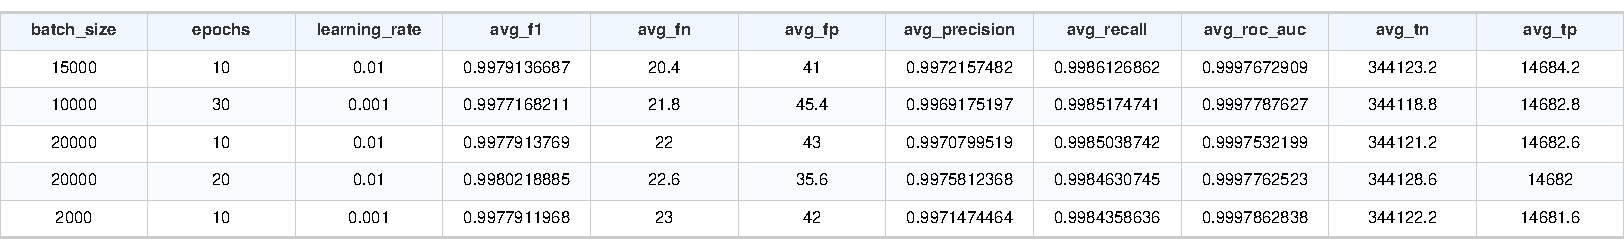
\includegraphics[width=1\textwidth]{./img/modelo/BINhs25.pdf}
    \caption{Mejores cinco configuraciones de hiperparámetros del modelo de clasificación binaria con una capa oculta de 25 neuronas.}
    \label{fig:BINhs25}
\end{figure}



La figura \ref{fig:BINhs49}, muestra la representación de las cinco mejores configuraciones de hiperparámetros para el modelo de clasificación binária con una arquitectura de 49 neuronas (n) en la capa oculta. Los resultados medios obtenidos concuerdan con lo comentado en el análisis de la sección \ref{sec:VIBIN49} para esta arquitectura. La mejor configuración para la arquitectura con la el mismo número de neuronas en la capa oculta que de parámetros de entrada tiene el modelo, ha sido:
\begin{itemize}
	\item \textbf{Batch size}: 20\,000
	\item \textbf{Epochs}: 10
	\item \textbf{Learning rate}: 0,01
\end{itemize}

\begin{figure}[H]
    \centering
    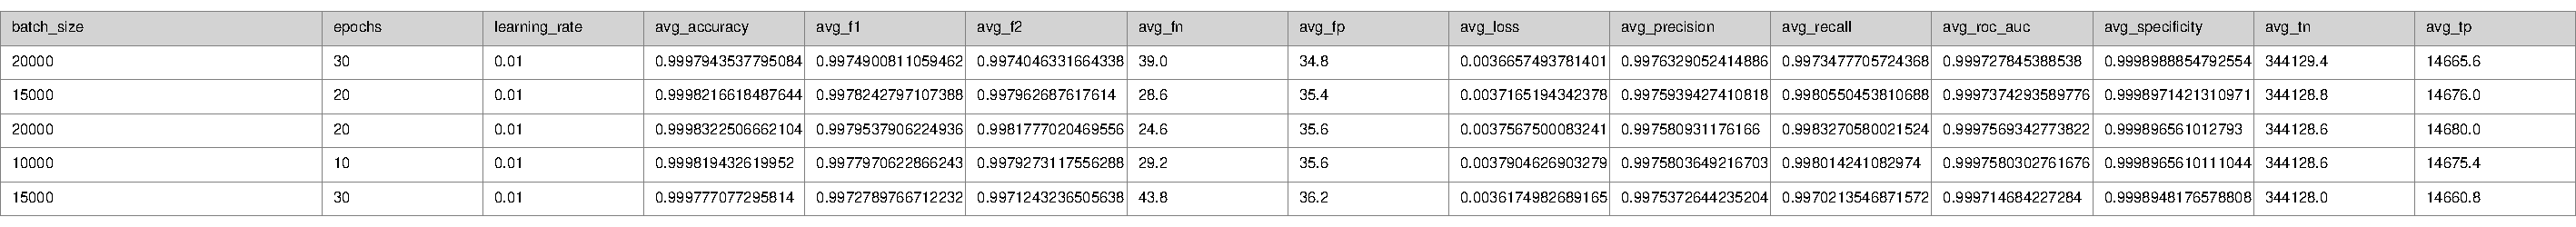
\includegraphics[width=1\textwidth]{./img/modelo/BINhs49.pdf}
    \caption{Mejores cinco configuraciones de hiperparámetros del modelo de clasificación binaria con una capa oculta de 49 neuronas.}
    \label{fig:BINhs49}
\end{figure}


En la figura \ref{fig:BINhs98}, se encuentran representadas las cinco mejores configuraciones de hiperparámetros para el modelo de clasificación binária con una arquitectura de 98 neuronas (n*2) en la capa oculta. Los resultados obtenidos coindiden con lo esperado tras el análisis de la sección \ref{sec:VIBIN98} para esta arquitectura. La mejor configuración para la arquitectura con el doble de neuronas en la capa oculta que de parámetros de entrada tiene el modelo, ha sido:
\begin{itemize}
	\item \textbf{Batch size}: 20\,000
	\item \textbf{Epochs}: 10
	\item \textbf{Learning rate}: 0,01
\end{itemize}

\begin{figure}[H]
    \centering
    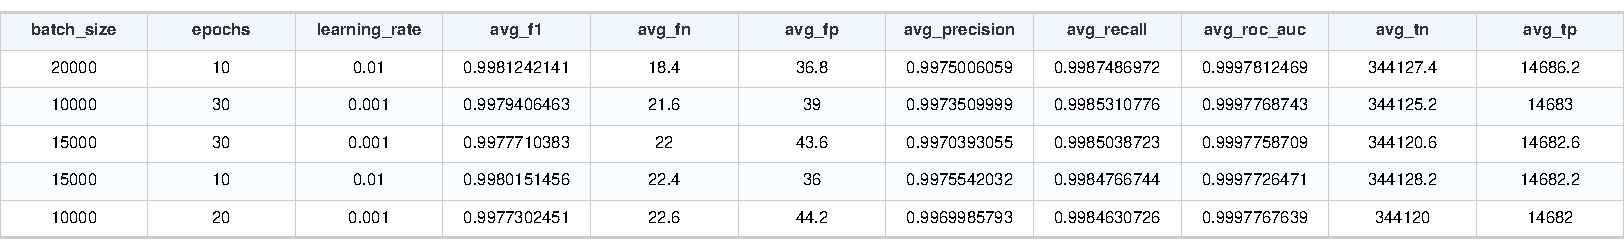
\includegraphics[width=1\textwidth]{./img/modelo/BINhs98.pdf}
    \caption{Mejores cinco configuraciones de hiperparámetros del modelo de clasificación binaria con una capa oculta de 98 neuronas.}
    \label{fig:BINhs98}
\end{figure}

Estos resultados no son definitivos, puesto que no se está evaluando la posibilidad de que el modelo haya sufrido sobreajuste incluso utilizando validación cruzada. Para obtener resultados reales del desempeño del modelo, se realizan pruebas, también conocidas como test, en las que se obtienen las métricas del modelo al recibir datos que no ha visto nunca. Este proceso y sus resultados se comentan en el capítulo \ref{cap.test}.


\subsection{Comparación de las arquitecturas}
En esta sección se comaparan los resultados obtenidos entre las tres arquitecturas propuestas. Una vez comparadas, se desarrolla una posible explicación para comprender los resultados de los experimientos.

Para comprender mejor los resultados globales de los experimentos, se han recogido en la figura \ref{fig:BINtop5}, las 5 configuraciones de hiperparámetros con mayor recall independientemente de su arquitectura.

\begin{figure}[H]
    \centering
    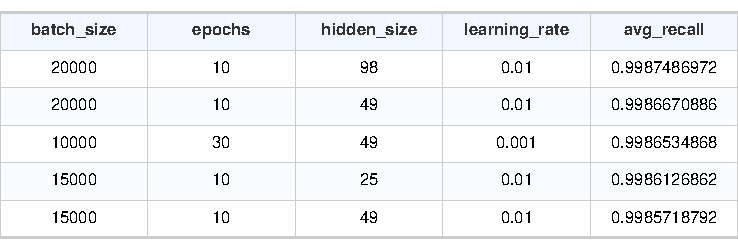
\includegraphics[width=0.85\textwidth]{./img/modelo/BINtop5.pdf}
    \caption{Mejores cinco configuraciones de hiperparámetros del modelo de clasificación binaria.}
    \label{fig:BINtop5}
\end{figure}

El problema para el que ha sido diseñado el modelo no presenta una relación lineal tras transformar los datos como se explica en el capítulo \ref{cap.ent-datos} \nameref{cap.ent-datos}. Por este motivo, se esperaba que el modelo con un tamaño de capa oculta mayor fuese capaz de converger mejor, tal y como se comenta en \ref{sec:VIBIN98}.

Al observar los datos de la figura \ref{fig:BINtop5}, se puede apreciar que puntualmente, la mejor arquitectura ha sido la que tenía un tamaño de ventana oculta igual a 98. Cabe destacar que, la diferencia entre los valores de recall de los cinco mejores experimentos es muy pequeña y puede que se deba a factores externos, como el estado de la máquina en el momento en el que se entreno al modelo, o la inicialización aleatoria de los pesos. Por este motivo, los resultados pueden variar si se realizan los mismos experimentos.

Ente los mejores resultados de los experimentos, detaca la presencia de la arquitectura con un tamaño de capa oculta igual al número de parámetros de entrada del modelo. Tal y como se comenta en las secciones anteriores, esta es la arquitectura más equilibrada. Gracias a este equilibrio ha sido capaz de ajustar sus pesos mejor que el rseto de arquitecturas para configuraciones de hiperparámetros diferentes.

Al aumentar el número de épocas del entrenamiento de los modelos, estos tienden a sobreajustar los pesos. Este sobreajuste implica que el modelo obtiene unas métricas excepcionalmente positivas durante los experimentos. Sin embargo, aun que los valores de las métricas son muy positivos en los experimentos realizados, sorprende que el número de épocas del 80 \% de las 5 mejores configuraciones, es el menor de los valores con los que se han realizado los experimentos para el hiperparámetro epochs. Estos resultados reflejan que la probabilidad de que el modelo haya sobreajustado sus pesos es muy baja. Posiblemente, el uso de la validación cruzada que penaliza el sobreajuste de los pesos de los modelos, como se explica en secciones anteriores, sea el responsable de que los experimentos con un número de épocas más elevado hayan obtenido unos resultados peores.

Finalmente, es destacable que el learning rate de la mayoría de los 5 mejores experimentos del global de las arquitecturas tenga el valor más alto de los que se han probado. Esto puede interpretarse de manera positiva o negativa.
En el mejor de los casos, un learning rate alto muestra que los datos están bien estructurados y que el optimizador y las arquitecturas son robustos frente a valores altos de learning rate,
En el peor de los casos, la convergencia se realiza rápidamente pero de manera inestable, los resultados dependan en gran medida de los valores iniciales de los pesos o se este sobreajustando el modelo. Este último caso es el más improbable debido a las técnicas utilizadas que se han descrito y a los resultados analizados en el párrafo anterior.

Para conocer el verdadero desempeño del modelo y determinar si ha sufirdo sobreajuste de los pesos durante el entrenamiento, se realiza un test con datos que no ha visto el modelo durante el entrenamiento. Estas pruebas y análisis se describen en el capítulo \ref{cap.test} \nameref{cap.test}. Si los resultados obtenidos de estos test son similares a los resultados obtenidos de los experimentos, significa que el modelo converge correctamente hacia una solución real. En caso de que los resultados obtenidos de los test sean significativamente peores que los obtenidos durante los experimentos, el modelo habrá sobreajustado sus pesos. 

\section{Modelo neuronal de clasificación multiclase}
Esta sección aborda los objetivos y procedimientos aplicados en el desarrollo del modelo de clasificación multiclase. Se describe el proceso llevado a cabo para la selección de hiperparámetros, junto con las diversas arquitecturas propuestas, con el propósito de identificar la configuración que maximiza el desempeño del modelo. Asimismo, se realiza una comparación exhaustiva entre las arquitecturas implementadas para determinar la opción más eficiente.

Por último, se detallan las métricas empleadas para la evaluación y la elección de las combinaciones óptimas de hiperparámetros,de forma análoga a como se hace en la sección \ref{sec.modBIN} \nameref{sec.modBIN}.

\subsection{Proposito del modelo de clasificación multiclase}

El modelo de clasificación multiclase se ha diseñado con el objetivo de identificar de manera precisa y eficiente, a que tipo de ataque corresponde una conexión maliciosa que ya se ha clasificado previamente como intrusiva. Su función principal consiste en distinguir entre 9 clases diferentes de ataques que se detallan en la sección \ref{sec.tipo-ataques} \nameref{sec.tipo-ataques}, contribuyendo a la protección proactiva de los sistemas informáticos.

\subsection{Diseño del modelo e hiperparámetros seleccionados} \label{sec:disMUL}
En esta sección se detalla cual es el diseño del modelo de clasificación multiclase escogido, así como los valore de los hiperparámetros utilizados durante los experimentos en el entrenamiento del modelo y sus correspondientes justificaciones.

Para diseñar la arquitectura del modelo, se ha desarrollado la clase ModeloMulticlase. Esta clase está conformada por dos funciones, la primera corresponde con la inicialización de la clase, y la segunda con la arquitectura utilizada para este modelo.

Como se puede observar en la figura \ref{fig:modMUL}, el modelo está compuesto por dos capas. La capa1 tiene un número de entradas igual al número de parámetros que poseen los datos utilizados para entrenar al modelo y un número de salidas que depende del parámetro \textit{ventaOculta}, con el que se llama a la función de inicialización del modelo. El número de salidas de la capa1 será precisamente el que determine la arquitectura específica que se utiliza. Una vez que los datos pasan por la capa1, se utiliza la técnica Batch Normalization. 

Batch Normalization es una técnica que normaliza las activaciones de una capa para que tengan media cercana a 0 y varianza cercana a 1, calculadas a partir del batch actual del entrenamiento del modelo. Aplicar BatchNorm tras la primera capa en un modelo de clasificación multiclase ayuda a estabilizar, acelerar y regularizar el entrenamiento, mejorando la capacidad del modelo para aprender buenas representaciones desde las primeras fases del entrenamiento.

Las redes neuronales necesitan funciones no lineales para aprender relaciones complejas entre las entradas y salidas, por este motivo, se aplica la función de activación Rectified Linear Unit (ReLU) depués del batch normalization. Sin activaciones como ReLU, toda la red sería equivalente a una simple transformación lineal, sin capacidad de aprendizaje profundo. Que el modelo presente una alta capacidad de aprendizaje profundo es esencial para los modelos de clasifiación multiclase cuya complejidad es mucho mayor que la de los modelos de clasificación binaria.

Para finalizar, la capa2 recibe como entrada el número de salidas de la capa1 y al tratarse de la capa final de un modelo de clasificación multiclase, esta capa tendrá una salda por cada clase que es capaz de identificar el modelo.

Por lo general, en clasificación multiclase, la salida del modelo suele ser un vector de logits (valores sin escalar), uno por cada clase. La función de activación Softmax transforma esos logits en probabilidades, es decir, cada valor representa lo probable que es que los datos que han entrado al modelo, pertenezca a esa clase. Debido a que durante el entrenamiento, se utiliza el frameworks PyTorch, no es necesario aplicar softmax a la salida del modelo cuando se utiliza la función de pérdida CrossEntropyLoss La razón es que función CrossEntropyLoss, ya incluye softmax internamente por razones de eficiencia y estabilidad numérica.

\begin{figure}[H]
    \centering
    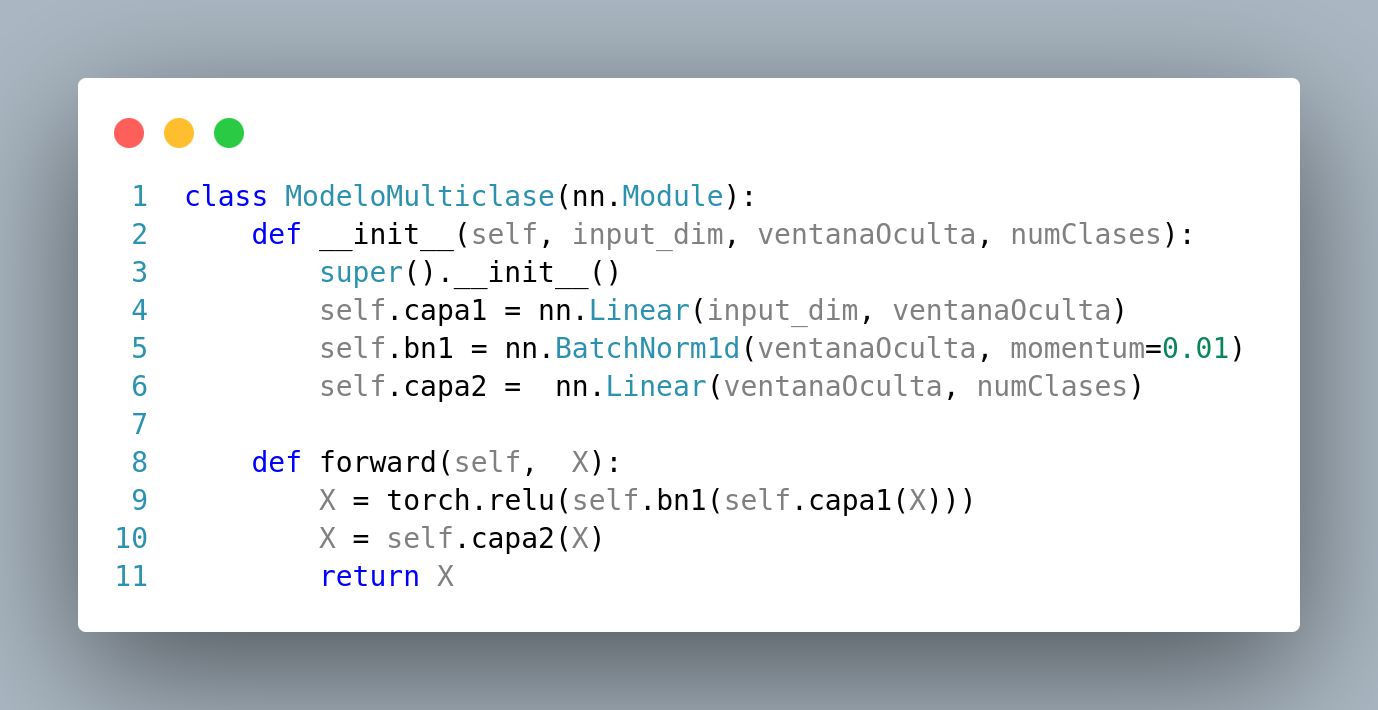
\includegraphics[width=0.8\textwidth]{./img/modelo/modeloMUL.png}
    \caption{Estructura del modelo de clasificación multiclase diseñada.}
    \label{fig:modMUL}
\end{figure}

Para evitar el sobreajuste del modelo y obtener valores de las predicciones más confiables que se utilizarán para la evaluación del rendimiento del modelo, se utiliza validación cruzada k-fold. Como se explica en la sección anterior \ref{sec:disBIN}, la validación cruzada consiste en dividir los datos de entrenamiento en n folds que se utilizan para entrenar al modelo con n-1 folds y después validar el modelo entrenado con el fold que no se ha utilizado para entrenarlo. Este proceso se repite para los n folds y en cada iteración es un fold distinto el que no se utiliza para el entrenamiento. Una vez completadas las iteraciones se extraen las medias de las métricas obtenidas con cada fold durante la validación. Para entrenar el modelo de clasificación multiclase, se ha utilizado StratifiedKFold() que como su nombre indica, estratifica los folds para que las proporciones de las clases de los datos utilizados para el entrenamiento se mantengan similares en cada fold y no se creen folds con un único tipo de clase. Estratificar los datos es especialmente crítico para aquellos datasets cuyos datos están muy desbalanceados como es el caso de los datos utilizados para entrenar los modelos de este proyecto. Concretamente, tras el tratamiento de los datos, existen 108 veces más muestras de la clase con mayor presencia en el dataset, que de la clase con menor presencias. Para el entrenamiento del modelo de clasificación multiclase, se ha optado por utilizar validación cruzada StratifiedKFold con 5 folds o divisiones.

Como algoritmo de optimización para el entrenamiento del modelo de clasificación multiclase, se ha optado por utilizar AdamW(). Como se comenta en la sección \ref{sec:alg-opt} \nameref{sec:alg-opt}, se ha demostrado que AdamW es más eficaz en la prevención de sobreajuste en redes neuronales que otros algoritmos de optimización.

Los hiperparámetros que han sido seleccionados para encontrar la mejor configuración para el modelo de clasificación multiclase diseñado son: el batch size, la tasa de aprendizaje (learning rate) y el número de épocas. Estos hiperparámetros resultan imprescindibles en el entrenamiento de modelos de clasificación multiclase, dado que influyen directamente en la eficiencia del proceso de optimización y en la calidad del modelo resultante.

Como se comenta en la sección \ref{sec:paramhiper} \refname{sec:paramhiper}, los hiperparámetros controlan el comportamiento del proceso de entrenamiento y afectan la capacidad del modelo para aprender patrones complejos de los datos. Teniendo en cuenta las características de cada hiperparámetro, se han escogido los siguientes valores para los experimentos del entrenamiento del modelo multiclase con el objetivo de encontrar la mejor combinación de ellos.

\begin{itemize}
	\item \textbf{Batch size}: Teniendo en cuenta el tamaño de los datos que se utilizan para la fase de entrenamiento del modelo de clasificación multiclase, se han considerado que los valores [32, 64, 128, 256, 512], eran apropiados y suficientemente dispares como para notar diferencias significativas en los resultados de la ejecución de los experimentos.
	\item \textbf{Learning rate}: Siguiendo los avisos de la sección anterior en la que se explicaba el propósito y características de cada hiperparámetro, se ha optado por elegir unos valores con los que se espera que el modelo converja sin sobreajustarse ni se exceda en el tiempo de obtención de una solución válida. Los valores elegidos han sido [0.01, 0.001, 0.0001, 0.00001].
	\item \textbf{Épocas}: De forma similar a como sucede con la tase de aprendizaje, un valor excesivamente bajo en el número de épocas puede provocar que el modelo no converja. Sin embargo, un número demasiado alto de épocas provoca sobreajuste en el modelo. Teniendo en cuenta las consideraciones mencionadas, los valores que se han probado para este hiperparámetro son [30, 50, 80, 100].
\end{itemize}

La convergencia de los modelos de clasifcación multiclase es mucho más complicada que en los modelos de clasificación binaria. Esto se debe a que en los modelos de clasificación binaria hay 4 posibles respuestas (VP, VN, FP, FN), mientras que en el  modelo de clasificación multiclase que se propone en este proyecto hay 9 clases por 9 posibilidades de respuesta por clase, lo que suma un total de 81 posibles respuestas. Para encontrar una configuración de los hiperparámetros que se ajuste mejor a la complejidad de este problema, se han probado más combinaciones de valores de los hiperparámetros en el modelo de clasificación multiclase que en el modelo de clasificación binaria. El aumento del número de experimentos se ha realizado teniendo en cuenta que el número de muestras de conexciones maliciosas es mucho menor que el número total de conexiones que se ha utilizado para entrenar el modelo de clasifcación binaria. Esto se traduce en que el tiempo de ejecución de los experimentos de ambos modelos ha sido similar compensando el número de muestras con el número de experimentos.

\subsection{Diseños del modelo de clasificación multiclase descartados}
Debido a la complejidad del problema al resolver, se probaron otros diseños que finalmente fueron descartados por no obtner los resultados esperados. A continuación, se detalla cuales fueron estos diseños descartados, la motivación que llevo a probarlo y cuales fueron sus resultados.

Durante las pruebas realizadas antes de ejecutar los experimentos para encontrar la combinación de hiperparámetros que mejor convergían para este modelo, se detectó que el desbalanceo de las clases afectaba de manera significativa a los resultados que se obtenían. Con el objetivo de reducir el impacto del desbalanceo en el entrenamiento del modelo, se optó por probar diferentes combinaciones que se muestran en la figura \ref{fig:MULpruebas}, junto con los resultados que obtuvieron estas combinaciones de funciones en la métrica F1 weighted.


\begin{figure}[H]
    \centering
    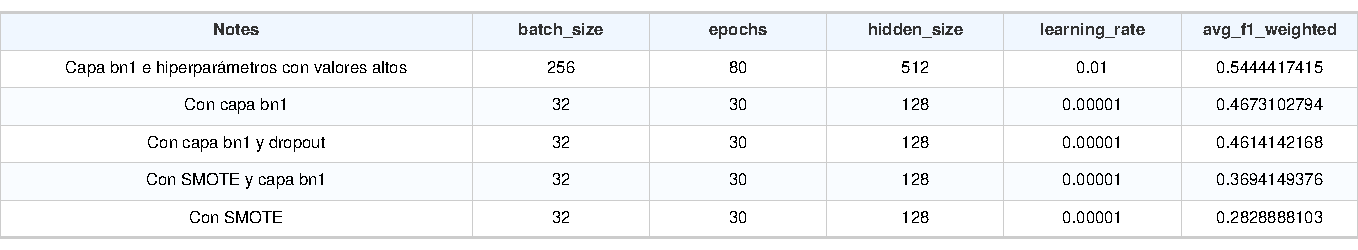
\includegraphics[width=0.95\textwidth]{./img/modelo/MULPRUEBAS.pdf}
    \caption{Resultados de los diferentes diseños probados para el modelo de clasifcación multiclase.}
    \label{fig:MULpruebas}
\end{figure}

SMOTE (Synthetic Minority Over-sampling Technique) es una técnica de sobremuestreo utilizada para abordar el problema del desbalance de clases en conjuntos de datos de clasificación. Su funcionamiento se basa en generar ejemplos sintéticos de las clases minoritarias, en lugar de replicar instancias existentes. En tareas de clasificación multiclase, SMOTE puede aplicarse a cada clase minoritaria de forma independiente, generando ejemplos sintéticos para aquellas clases con menor representación. La aplicación de esta técnica en modelos de clasificación multiclase muy desbalanceados:

\begin{itemize}
	\item Contribuye a reducir el sesgo del modelo hacia las clases mayoritarias.

	\item Mejora el rendimiento en métricas como recall y F1-score macro, al equilibrar el conjunto de entrenamiento.

	\item Favorece una mejor generalización en la predicción de clases minoritarias, al ampliar su representación en el espacio de características.
\end{itemize}

Sin embargo, tras realizar una serie de pruebas, el modelo diseñado que implementaba  SMOTE fue el que peores resultados dió. Por eso motivo, se combinó con la función Batch Normalization explicada en la sección \ref{sec:disMUL} \nameref{sec:disMUL}.

Los resultados de Batch Normalization (bn1) y SMOTE fueron algo mejores que los valores obtenidos de las pruebas realizadas solo con SMOTE. Como se noto una mejora en el desempeño del modelo al utilizar bn1, pero los resultados obtenidos seguían sin ser los esperados,se probó con combinaciones de diseño utilizando bn1 con otras técnicas.

Dropout es una técnica de regularización utilizada en redes neuronales para reducir el sobreajuste durante el entrenamiento. La función Dropout(), implementada en bibliotecas como TensorFlow y PyTorch, actúa introduciendo aleatoriamente una probabilidad de desactivación sobre las neuronas de una capa determinada. Durante cada iteración de entrenamiento, un subconjunto aleatorio de neuronas es temporalmente desactivado (es decir, sus salidas se anulan) con una probabilidad definida, denominada tasa de dropout (dropout rate), sin afectar la arquitectura del modelo ni sus pesos de forma permanente. Los principales beneficios de utilizar dropout en un modelo de clasificación multicase con unos datos de entrenamiento muy desbalanceados son:

\begin{itemize}
	\item Reduce el sobreajuste hacia las clases mayoritarias, evitando que el modelo memorice solo los patrones frecuentes y mejorando su comportamiento general.

	\item Fomenta la generalización en clases minoritarias, al impedir dependencias excesivas entre neuronas y promover representaciones más robustas y diversas.

	\item Mejora métricas sensibles al desbalance como el weighted F1-score o macro recall, al favorecer que el modelo aprenda también de clases con baja representación.
\end{itemize}

Con la implementación del dropout, los resultados mejoraron significativamente. Sin embargo, el diseño del modelo que solo utilizaba bn1 obtuvo mejores resultados de media que aquel que utilizaba bn1 y dropout. Por este motivo, el diseño utilizado en los experimentos solo implementa Batch Normalization. Además, tras realizar pruebas con valores altos para los hiperparámetros, se obtuvieron unos resultados con una convergencia mayor que la de las pruebas realizadas con valores menores, lo que incentivó a aumentar los valores de los hiperparámetros probados, tal y como se puede observar en la sección anterior.



\subsection{Arquitecturas desarrolladas}
En esta sección se abordan cuales son las arquitecturas a desarrollar para el modelo de clasificación multiclase. Como se comenta en la sección anterior \ref{sec:disMUL} \nameref{sec:disMUL}, la diferencia entre las arquitecturas radica en el tamaño de la capa oculta del modelo.

Para el desarrollo de las diferentes arquitecturas, se ha optado por realizar experimentos de entrenamiento del modelo de clasificación multiclase con un tamaño de ventana oculta igual a:
la mitad del número de parámetros que recibe el modelo, el mismo número que parámetros que tiene el modelo y doble del número de parámetros. Esto equivale a un tamaño de la capa de venta oculta de 25, 49 y 98 respectivamente, de forma análoga a como sucede con las arquitecturas del modelod de clasificación binaria. Estos valores se obtienen de forma dinámica después de tratar los datos del csv utilizado para los entrenamientos y las pruebas de este proyecto.

A continuación, se comentan las posibles ventajas e inconvenientes de cada arquitectura que se esperan antes de realizar los experimentos.

\subsubsection{Capa oculta con la mitad de neuronas que parámetros de entrada}\label{sec:VIMUL25}
En este apartado se comentan cuales son las principales ventajas e inconvenientes, a priori, de un modelo de clasificación multiclase con un número de neuronas en la capa oculta igual a la mitad del número de parámetros que recibe el modelo.

\paragraph{Ventajas (n/2)}
\begin{itemize}
	\item Un número reducido de neuronas en la capa oculta limita la capacidad del modelo para memorizar patrones dominantes, lo cual puede ayudar a mitigar el sobreajuste hacia las clases mayoritarias del conjunto de entrenamiento.
	\item Al reducirse la complejidad del modelo, se disminuye el tiempo necesario para calcular los gradientes durante el entrenamiento y, en consecuencia, también el tiempo de respuesta durante la inferencia.
	\item En presencia de clases desbalanceadas, un modelo menos expresivo puede favorecer una mayor estabilidad en el aprendizaje, evitando que la red se especialice únicamente en las clases más frecuentes.

\end{itemize}
\paragraph{Inconvenientes(n/2)}
\begin{itemize}
	\item Un número bajo de neuronas puede limitar la capacidad del modelo para aprender representaciones suficientes de las clases minoritarias, especialmente si estas presentan patrones complejos o poco diferenciados.
	\item La capacidad reducida del modelo puede dificultar la separación entre clases en problemas multiclase, afectando negativamente al rendimiento en métricas sensibles al desbalance como el macro recall o el macro F1-score.
	\item Si el número de parámetros de entrada es muy alto, una capa oculta con solo la mitad de neuronas podría actuar como un cuello de botella, perdiéndose información útil para distinguir correctamente entre clases poco representadas.

\end{itemize}

Tras comentar cuales son las principales ventajas e inconvenientes de utilizar una capa oculta con un número de neuronas igual a la mitad de los parámetros del modelo, aparentemente, las propiedades del conjunto de datos que se utiliza para entrenar al modelo no son las idóneas para esta arquitectura y no se esperan resultados especialmente destacables. Debido al alto desbalanceo entre clases, se espera que esta arquitectura proporcione resultados peores que su equivalente del modelo de clasificación binaria.

\subsubsection{Capa oculta con el mismo número de neuronas que parámetros de entrada}\label{sec:VIMUL49}
En este apartado se comentan cuales son las principales ventajas e inconvenientes, a priori, de un modelo de clasificación multiclase con un número de neuronas en la capa oculta igual al número de parámetros que recibe el modelo.

\paragraph{Ventajas (n)}
\begin{itemize}
	\item Un número de neuronas igual al de parámetros de entrada proporciona al modelo una capacidad representativa suficiente para capturar patrones relevantes tanto en clases frecuentes como en las minoritarias.
	\item Esta configuración ofrece un equilibrio razonable entre complejidad y eficiencia computacional, manteniendo un coste de entrenamiento y de inferencia moderado sin comprometer la expresividad del modelo.
	\item Permite al modelo adaptar sus pesos de manera más flexible, facilitando el aprendizaje de límites de decisión más precisos entre clases desbalanceadas sin riesgo inmediato de sobreajuste.

\end{itemize}
\paragraph{Inconvenientes(n)}
\begin{itemize}
	\item Aun sin ser excesivo, este tamaño puede generar cierta sobreadaptación a las clases mayoritarias si no se aplican mecanismos de regularización adecuados.
	\item En conjuntos de datos muy desbalanceados, esta configuración puede no ser suficiente para compensar la escasa representación de clases minoritarias, especialmente si estas requieren una mayor capacidad para ser correctamente diferenciadas.
	\item Si las características de entrada tienen una alta correlación entre sí, mantener el mismo número de neuronas puede introducir redundancia, afectando la eficiencia del aprendizaje y aumentando el riesgo de converger a soluciones deficientes.
\end{itemize}

Tras comentar cuales son las principales ventajas e inconvenientes de utilizar una capa oculta con el mismo número de neuronas que parámetros recibe el modelo, aparentemente, esta arquitectura ofrecera resultados significativamente positivos gracias a su equilibrio. Aun que, si las clases que tienen un número inferior de muestras, tienen relaciones complejas entre sus datos, esta arquitectura puede ser insuficiente para obtener un modelo capaz de distinguir entre algunas de las clases más minoritarias.

\subsubsection{Capa oculta con el doble de neuronas que parámetros de entrada}\label{sec:VIMUL98}
En este apartado se comentan cuales son las principales ventajas e inconvenientes, a priori, de un modelo de clasificación multiclase con el doble de neuronas en la capa oculta que parámetros recibe el modelo.

\paragraph{Ventajas (n*2)}
\begin{itemize}
	\item Una capa oculta más amplia incrementa la capacidad del modelo para aprender representaciones complejas, lo que puede ser especialmente útil para distinguir correctamente clases minoritarias con patrones sutiles o poco definidos.
	\item Esta configuración ofrece una mayor flexibilidad al modelo para aproximar funciones no lineales, favoreciendo una mejor separación entre clases en escenarios multiclase con alta variabilidad entre categorías.
	\item Al disponer de más neuronas, el modelo tiene mayor margen para explorar combinaciones de características relevantes durante el entrenamiento, lo cual puede traducirse en una mejora de métricas como macro F1 o recall por clase.
\end{itemize}

\paragraph{Inconvenientes(n*2)}
\begin{itemize}
	\item El aumento en el número de parámetros incrementa el riesgo de sobreajuste, especialmente en presencia de clases mayoritarias dominantes o cuando el conjunto de entrenamiento es reducido
	\item Un modelo con mayor complejidad requiere más recursos computacionales y tiempos de entrenamiento más prolongados, lo que puede dificultar su implementación en entornos con restricciones de capacidad o temporales.
	\item Si no se utilizan mecanismos de control adecuados (como regularización o balanceo de clases), es posible que el modelo aprenda a ajustar principalmente las clases frecuentes, sin mejorar sustancialmente el rendimiento en las minoritarias.

\end{itemize}

Tras comentar cuales son las principales ventajas e inconvenientes de utilizar una capa oculta con un número de neuronas igual al doble de los parámetros del modelo, aparentemente, esta arqutectura será la que mejores resultados obtenga en la detección de clases minoritarias al tener la capacidad de aprender representaciones más complejas. Sin embargo, esta arquitectura es más propensa a sobreajustes debido la presencia de las clases mayoritarias.


\subsection{Matriz de confusión para clasificación multiclase} \label{sec.matriz-consfusion-multi}

Como se explica en la sección anterior \ref{sec.matriz-consfusion}\nameref{sec.matriz-consfusion}, la matriz de confusión 


Para un modelo con múltiples clases, como es el caso del modelo de que se desarrolla en este docuimento,se debe tener en cuenta que en un modelo neuronal con 9 salidas, la matriz tiene las siguientes interpretaciones:
\begin{itemize}
	\item Diagonal principal: Cada celda de la diagonal principal de la matriz representa cuántas veces la clase real fue correctamente predicha como clase. Este es el caso de las instancias que fueron correctamente clasificadas, y es lo más cercano a un "verdadero positivo" para esa clase específica. Sin embargo, en clasificación multiclase, se suele hablar de aciertos o instancias correctamente clasificadas para cada clase.

	\item Fuera de la diagonal: Las celdas fuera de la diagonal representan falsas clasificaciones. Es decir, representan cuántas veces una instancia de la clase real fue predicha incorrectamente como otra clase.

\end{itemize}


\begin{table}[h]
\centering
\label{tab:confusion_matrix_9class}
\resizebox{\textwidth}{!}{
\begin{tabular}{|l|c|c|c|c|c|c|c|c|c|}
\hline
 & \textbf{Predicción Clase 1} & \textbf{Predicción Clase 2} & \textbf{Predicción Clase 3} & \textbf{Predicción Clase 4} & \textbf{Predicción Clase 5} & \textbf{Predicción Clase 6} & \textbf{Predicción Clase 7} & \textbf{Predicción Clase 8} & \textbf{Predicción Clase 9} \\ \hline
\textbf{Real Clase 1} & VP$_{1}$ & FP$_{12}$ & FP$_{13}$ & FP$_{14}$ & FP$_{15}$ & FP$_{16}$ & FP$_{17}$ & FP$_{18}$ & FP$_{19}$ \\ \hline
\textbf{Real Clase 2} & FP$_{21}$ & VP$_{2}$ & FP$_{23}$ & FP$_{24}$ & FP$_{25}$ & FP$_{26}$ & FP$_{27}$ & FP$_{28}$ & FP$_{29}$ \\ \hline
\textbf{Real Clase 3} & FP$_{31}$ & FP$_{32}$ & VP$_{3}$ & FP$_{34}$ & FP$_{35}$ & FP$_{36}$ & FP$_{37}$ & FP$_{38}$ & FP$_{39}$ \\ \hline
\textbf{Real Clase 4} & FP$_{41}$ & FP$_{42}$ & FP$_{43}$ & VP$_{4}$ & FP$_{45}$ & FP$_{46}$ & FP$_{47}$ & FP$_{48}$ & FP$_{49}$ \\ \hline
\textbf{Real Clase 5} & FP$_{51}$ & FP$_{52}$ & FP$_{53}$ & FP$_{54}$ & VP$_{5}$ & FP$_{56}$ & FP$_{57}$ & FP$_{58}$ & FP$_{59}$ \\ \hline
\textbf{Real Clase 6} & FP$_{61}$ & FP$_{62}$ & FP$_{63}$ & FP$_{64}$ & FP$_{65}$ & VP$_{6}$ & FP$_{67}$ & FP$_{68}$ & FP$_{69}$ \\ \hline
\textbf{Real Clase 7} & FP$_{71}$ & FP$_{72}$ & FP$_{73}$ & FP$_{74}$ & FP$_{75}$ & FP$_{76}$ & VP$_{7}$ & FP$_{78}$ & FP$_{79}$ \\ \hline
\textbf{Real Clase 8} & FP$_{81}$ & FP$_{82}$ & FP$_{83}$ & FP$_{84}$ & FP$_{85}$ & FP$_{86}$ & FP$_{87}$ & VP$_{8}$ & FP$_{89}$ \\ \hline
\textbf{Real Clase 9} & FP$_{91}$ & FP$_{92}$ & FP$_{93}$ & FP$_{94}$ & FP$_{95}$ & FP$_{96}$ & FP$_{97}$ & FP$_{98}$ & VP$_{9}$ \\ \hline
\end{tabular}
}
\caption{Matriz de confusión para clasificación con 9 clases.}
\end{table}


\subsection{Metricas útiles en clasificación multiclase} \label{sec:metricas-mul}

En el desarrollo de modelos neuronales para clasificación multiclase, es fundamental contar con métricas que permitan evaluar el desempeño general y específico del modelo. A continuación, se presentan las métricas más relevantes, agrupadas según su naturaleza: generales, macro-promediadas y ponderadas.
\subsubsection*{Métricas Generales}

\begin{itemize}

\item \textbf{Exactitud (\textit{Accuracy})}:

\begin{equation}
\text{Accuracy} = \frac{1}{N} \sum_{i=1}^{N} \mathbf{1}_{\{y_i = \hat{y}_i\}}
\end{equation}

La exactitud cuantifica la proporción de predicciones correctas sobre el total de instancias evaluadas. En contextos de clasificación multiclase, proporciona una medida global del rendimiento del modelo. Sin embargo, su uso puede resultar limitado en escenarios donde las clases están desbalanceadas, ya que tiende a favorecer aquellas clases con mayor representación. En estos casos, una alta exactitud puede enmascarar un bajo rendimiento en clases minoritarias, lo que podría comprometer la robustez del modelo. Se considera una métrica de referencia general, pero insuficiente para evaluar en profundidad el comportamiento del modelo en todos los grupos de clase.

\end{itemize}

\subsubsection*{Métricas Macro-promediadas}

Las métricas macro-promediadas se calculan evaluando individualmente el rendimiento del modelo para cada clase y luego promediando estos resultados. Esta metodología asigna igual peso a todas las clases, independientemente de su frecuencia, lo que permite detectar deficiencias de desempeño en clases poco representadas. Son particularmente útiles en problemas de clasificación multiclase con desequilibrios significativos.

\begin{itemize}

\item \textbf{Precisión Macro (\textit{Macro Precision})}:

\begin{equation}
\text{Precision}_{\text{macro}} = \frac{1}{C} \sum_{c=1}^{C} \text{Precision}_c
\end{equation}

La precisión macro evalúa la proporción de verdaderos positivos entre todas las predicciones positivas, calculada individualmente para cada clase y promediada de forma equitativa. Esta métrica permite identificar si el modelo tiende a emitir predicciones incorrectas en ciertas clases, lo cual puede ser crítico en aplicaciones donde los falsos positivos resultan costosos. En entornos multiclase, su utilidad radica en evaluar la calidad de las predicciones para todas las clases de forma uniforme.

\item \textbf{Sensibilidad Macro (\textit{•}{Macro Recall})}:

\begin{equation}
\text{Recall}_{\text{macro}} = \frac{1}{C} \sum_{c=1}^{C} \text{Recall}_c
\end{equation}

La sensibilidad macro (o exhaustividad) mide la proporción de verdaderos positivos sobre el total de instancias reales de cada clase. Al promediarla sin ponderar por la frecuencia de clase, esta métrica refleja la capacidad del modelo de detectar correctamente todas las clases, incluidas aquellas menos frecuentes. Resulta esencial en situaciones donde los falsos negativos tienen consecuencias graves o donde se busca una cobertura completa del espacio de clases.

\item \textbf{F1 Macro (\textit{Macro F1 Score})}:

\begin{equation}
F1_{\text{macro}} = \frac{1}{C} \sum_{c=1}^{C} F1_c
\end{equation}

El F1 macro se obtiene calculando el F1 score individual por clase (media armónica entre precisión y sensibilidad), y promediándolo uniformemente. Esta métrica proporciona una visión equilibrada del desempeño del modelo en todas las clases, y es especialmente útil cuando se busca un rendimiento homogéneo en un entorno multiclase, independientemente de la distribución de las muestras.

\end{itemize}

\subsubsection*{Métricas Ponderadas (\textit{Weighted})}

Las métricas ponderadas (weighted) también se calculan por clase, pero se ajustan según la frecuencia de aparición de cada clase en el conjunto de datos. Este enfoque permite obtener una representación más realista del rendimiento global del modelo, otorgando mayor peso a las clases con mayor número de instancias. Son adecuadas para obtener una evaluación que respete la distribución natural del conjunto de datos, sin perder información relevante de las clases menos representadas.

\begin{itemize}

\item \textbf{Precisión Ponderada (\textit{Weighted Precision})}:

\begin{equation}
\text{Precision}_{\text{weighted}} = \sum_{c=1}^{C} \frac{N_c}{N} \cdot \text{Precision}_c
\end{equation}

La precisión ponderada evalúa la calidad de las predicciones positivas, ajustada por la proporción de instancias de cada clase. Esta métrica resulta útil para capturar el rendimiento general del modelo en conjuntos de datos con distribución desigual, sin que las clases poco frecuentes dominen el resultado final.

\item \textbf{Sensibilidad Ponderada (\textit{Weighted Recall})}:

\begin{equation}
\text{Recall}_{\text{weighted}} = \sum_{c=1}^{C} \frac{N_c}{N} \cdot \text{Recall}_c
\end{equation}

La sensibilidad ponderada proporciona una medida del porcentaje de instancias reales correctamente identificadas, teniendo en cuenta la frecuencia de cada clase. En modelos de clasificación multiclase, permite analizar cómo se comporta el modelo con respecto a la cobertura general de los datos, favoreciendo una evaluación proporcional al tamaño de las clases.

\item \textbf{F1 Ponderado (\textit{Weighted F1 Score})}:

\begin{equation}
F1_{\text{weighted}} = \sum_{c=1}^{C} \frac{N_c}{N} \cdot F1_c
\end{equation}

El F1 ponderado combina precisión y sensibilidad ajustadas por la proporción de cada clase. Es una de las métricas más importantes cuando se desea evaluar un rendimiento global equilibrado que refleje el impacto relativo de cada clase en el conjunto de datos, resultando especialmente útil para comparar modelos entrenados sobre datasets desbalanceados.

\end{itemize}

\subsubsection*{Área Bajo la Curva ROC (AUC)}

El área bajo la curva ROC (AUC) mide la capacidad del modelo para distinguir entre clases. En clasificación multiclase, se emplean dos métodos principales para su cálculo:

\begin{itemize}

\item \textbf{AUC One-vs-One (OVO)}:

\begin{equation}
\text{AUC}_{\text{ovo}} = \frac{1}{C(C-1)/2} \sum_{i<j} \text{AUC}_{i,j}
\end{equation}

El enfoque One-vs-One calcula el AUC para cada par de clases, evaluando la capacidad del modelo para distinguir una clase frente a otra. El resultado final se obtiene promediando los valores obtenidos para todos los pares posibles. Esta estrategia proporciona una evaluación detallada de la separabilidad entre clases específicas. Es útil cuando se quiere analizar el comportamiento del modelo en decisiones binarias dentro del espacio multiclase.

\item \textbf{AUC One-vs-Rest (OVR)}:

\begin{equation}
\text{AUC}_{\text{ovr}} = \frac{1}{C} \sum_{c=1}^{C} \text{AUC}_c
\end{equation}

El enfoque One-vs-Rest evalúa, para cada clase, la capacidad del modelo de distinguir dicha clase frente a todas las demás combinadas. Esta métrica permite examinar el rendimiento del modelo desde la perspectiva de cada clase individual y es adecuada para diagnósticos detallados en entornos multiclase.

\end{itemize}


\subsection{Mejores hiperparámetros para cada arquitectura}
En esta sección se pueden observar los resultados de los experimentos realizados con los posibles valores de los hiperparámetros comentados en la sección \ref{sec:disMUL} \nameref{sec:disMUL}.

Para medir la eficiencia y eficacia del modelo, se han obtenido las métricas derivadas de la matriz de confusión comentadas en la sección \ref{sec.metricas-mul} \nameref{sec.metricas-mul}. El objetivo de este modelo es clasificar intrusiones en redes, ya detectadas en diferentes tipos específicos de ataque enumerados en la sección \ref{sec.tipo-ataques} para facilitar una respuesta adecuada. Aunque una clasificación incorrecta puede afectar la eficiencia de la mitigación, las consecuencias no son tan catastróficas como en el caso de falso negativo del modelo de clasificación binaria. Sin embargo, la precisión en la identificación del tipo de ataque sigue siendo clave para optimizar los recursos y la estrategia de defensa.
Teniendo esto en cuenta, la métrica más importante es Weifhted F1 socre, ya que como se comenta en el apartado anterior, refleja el impacto relativo de cada clase en el conjunto de datos, resultando especialmente útil para comparar modelos entrenados con datasets desbalanceados.

Otras métricas relevantes que se muestran en las siguientes figuras son:
\begin{itemize}
	\item \textbf{ Macro F1 Score}: Indica un buen equilibrio entre precisión y recall promedio por clase, sin importar su frecuencia, lo que refleja buen rendimiento en todas las clases, incluidas las minoritarias.
	\item \textbf{ Macro Recall}: Un valor alto significa que el modelo detecta correctamente una alta proporción de instancias reales en cada clase, lo que es crucial para no ignorar clases poco representadas.
	\item \textbf{Macro Precision}: mide qué proporción de predicciones por clase son correctas. Un valor alto implica que el modelo no clasifica erróneamente otras clases como una clase minoritaria.
\end{itemize}

En la figura \ref{fig:MULhs25}, se encuentran representadas las cinco mejores configuraciones de hiperparámetros para el modelo de clasificación multiclase con una arquitectura de 25 neuronas (n/2) en la capa oculta. Coinciden con lo esperado tras el análisis de la sección \ref{sec:VIBIN25} para esta arquitectura. La mejor configuración para la arquitectura con la mitad de neuronas en la capa oculta que de parámetros de entrada tiene el modelo, ha sido:
\begin{itemize}
	\item \textbf{Batch size}: 15\,000
	\item \textbf{Epochs}: 10
	\item \textbf{Learning rate}: 0,01
\end{itemize}
Estos resultados no son definitivos, puesto que no se está evaluando la posibilidad de que el modelo haya sufrido sobreajuste incluso utilizando validación cruzada. Para obtener resultados reales del desempeño del modelo, se realizan pruebas, también conocidas como test, en las que se obtienen las métricas del modelo al recibir datos que no ha visto nunca. Este proceso y sus resultados se comentan en el capítulo \ref{cap.test} \nameref{cap.test}.

\begin{figure}[H]
    \centering
    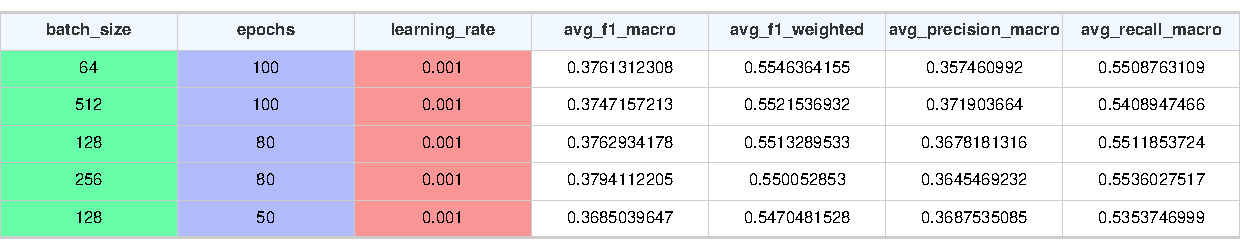
\includegraphics[width=1\textwidth]{./img/modelo/MULhs25.pdf}
    \caption{Mejores cinco configuraciones de hiperparámetros del modelo de clasificación binaria con una capa oculta de 25 neuronas.}
    \label{fig:MULhs25}
\end{figure}



La figura \ref{fig:BINhs49}, muestra la representación de las cinco mejores configuraciones de hiperparámetros para el modelo de clasificación binária con una arquitectura de 49 neuronas (n) en la capa oculta. Los resultados medios obtenidos concuerdan con lo comentado en el análisis de la sección \ref{sec:VIBIN49} para esta arquitectura. La mejor configuración para la arquitectura con la el mismo número de neuronas en la capa oculta que de parámetros de entrada tiene el modelo, ha sido:
\begin{itemize}
	\item \textbf{Batch size}: 20\,000
	\item \textbf{Epochs}: 10
	\item \textbf{Learning rate}: 0,01
\end{itemize}

\begin{figure}[H]
    \centering
    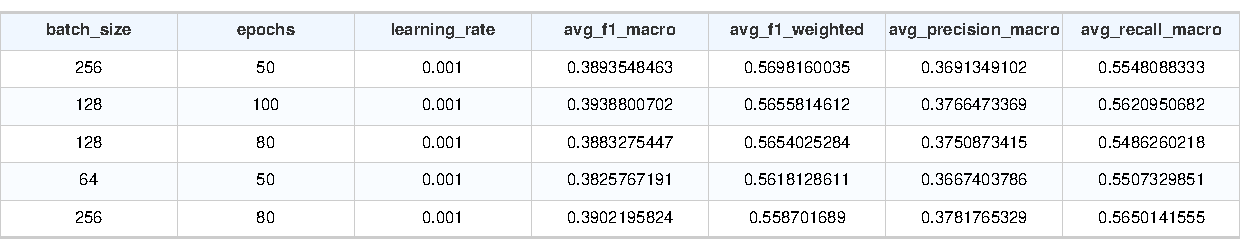
\includegraphics[width=1\textwidth]{./img/modelo/MULhs49.pdf}
    \caption{Mejores cinco configuraciones de hiperparámetros del modelo de clasificación binaria con una capa oculta de 49 neuronas.}
    \label{fig:MULhs49}
\end{figure}


En la figura \ref{fig:BINhs98}, se encuentran representadas las cinco mejores configuraciones de hiperparámetros para el modelo de clasificación binária con una arquitectura de 98 neuronas (n*2) en la capa oculta. Los resultados obtenidos coindiden con lo esperado tras el análisis de la sección \ref{sec:VIBIN98} para esta arquitectura. La mejor configuración para la arquitectura con el doble de neuronas en la capa oculta que de parámetros de entrada tiene el modelo, ha sido:
\begin{itemize}
	\item \textbf{Batch size}: 20\,000
	\item \textbf{Epochs}: 10
	\item \textbf{Learning rate}: 0,01
\end{itemize}

\begin{figure}[H]
    \centering
    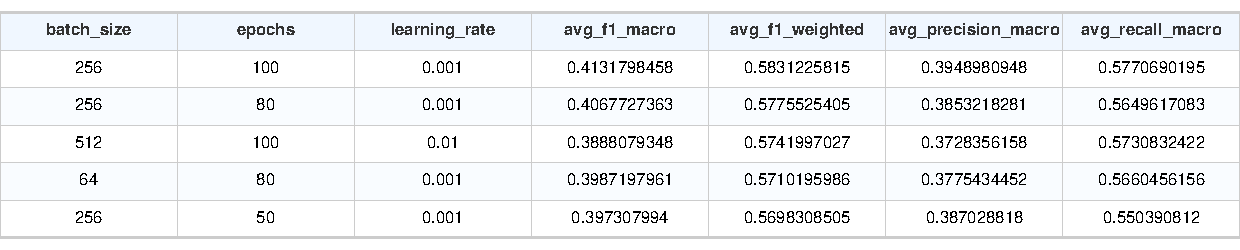
\includegraphics[width=1\textwidth]{./img/modelo/MULhs98.pdf}
    \caption{Mejores cinco configuraciones de hiperparámetros del modelo de clasificación binaria con una capa oculta de 98 neuronas.}
    \label{fig:MULhs98}
\end{figure}

Estos resultados no son definitivos, puesto que no se está evaluando la posibilidad de que el modelo haya sufrido sobreajuste incluso utilizando validación cruzada. Para obtener resultados reales del desempeño del modelo, se realizan pruebas, también conocidas como test, en las que se obtienen las métricas del modelo al recibir datos que no ha visto nunca. Este proceso y sus resultados se comentan en el capítulo \ref{cap.test}.


\subsection{Comparación de las arquitecturas}
En esta sección se comaparan los resultados obtenidos entre las tres arquitecturas propuestas. Una vez comparadas, se desarrolla una posible explicación para comprender los resultados de los experimientos.

Para comprender mejor los resultados globales de los experimentos, se han recogido en la figura \ref{fig:BINtop5}, las 5 configuraciones de hiperparámetros con mayor recall independientemente de su arquitectura.

\begin{figure}[H]
    \centering
    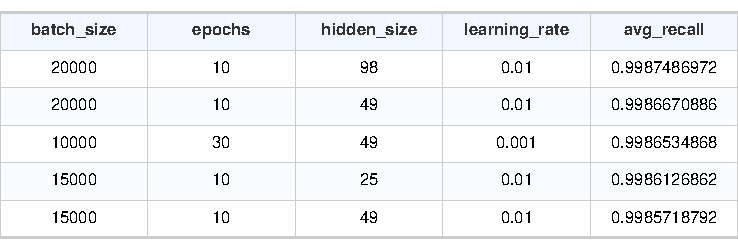
\includegraphics[width=0.85\textwidth]{./img/modelo/BINtop5.pdf}
    \caption{Mejores cinco configuraciones de hiperparámetros del modelo de clasificación binaria.}
    \label{fig:BINtop5}
\end{figure}

El problema para el que ha sido diseñado el modelo no presenta una relación lineal tras transformar los datos como se explica en el capítulo \ref{cap.ent-datos} \nameref{cap.ent-datos}. Por este motivo, se esperaba que el modelo con un tamaño de capa oculta mayor fuese capaz de converger mejor, tal y como se comenta en \ref{sec:VIBIN98}.

Al observar los datos de la figura \ref{fig:BINtop5}, se puede apreciar que puntualmente, la mejor arquitectura ha sido la que tenía un tamaño de ventana oculta igual a 98. Cabe destacar que, la diferencia entre los valores de recall de los cinco mejores experimentos es muy pequeña y puede que se deba a factores externos, como el estado de la máquina en el momento en el que se entreno al modelo, o la inicialización aleatoria de los pesos. Por este motivo, los resultados pueden variar si se realizan los mismos experimentos.

Ente los mejores resultados de los experimentos, detaca la presencia de la arquitectura con un tamaño de capa oculta igual al número de parámetros de entrada del modelo. Tal y como se comenta en las secciones anteriores, esta es la arquitectura más equilibrada. Gracias a este equilibrio ha sido capaz de ajustar sus pesos mejor que el rseto de arquitecturas para configuraciones de hiperparámetros diferentes.

Al aumentar el número de épocas del entrenamiento de los modelos, estos tienden a sobreajustar los pesos. Este sobreajuste implica que el modelo obtiene unas métricas excepcionalmente positivas durante los experimentos. Sin embargo, aun que los valores de las métricas son muy positivos en los experimentos realizados, sorprende que el número de épocas del 80 \% de las 5 mejores configuraciones, es el menor de los valores con los que se han realizado los experimentos para el hiperparámetro epochs. Estos resultados reflejan que la probabilidad de que el modelo haya sobreajustado sus pesos es muy baja. Posiblemente, el uso de la validación cruzada que penaliza el sobreajuste de los pesos de los modelos, como se explica en secciones anteriores, sea el responsable de que los experimentos con un número de épocas más elevado hayan obtenido unos resultados peores.

Finalmente, es destacable que el learning rate de la mayoría de los 5 mejores experimentos del global de las arquitecturas tenga el valor más alto de los que se han probado. Esto puede interpretarse de manera positiva o negativa.
En el mejor de los casos, un learning rate alto muestra que los datos están bien estructurados y que el optimizador y las arquitecturas son robustos frente a valores altos de learning rate,
En el peor de los casos, la convergencia se realiza rápidamente pero de manera inestable, los resultados dependan en gran medida de los valores iniciales de los pesos o se este sobreajustando el modelo. Este último caso es el más improbable debido a las técnicas utilizadas que se han descrito y a los resultados analizados en el párrafo anterior.

Para conocer el verdadero desempeño del modelo y determinar si ha sufirdo sobreajuste de los pesos durante el entrenamiento, se realiza un test con datos que no ha visto el modelo durante el entrenamiento. Estas pruebas y análisis se describen en el capítulo \ref{cap.test} \nameref{cap.test}. Si los resultados obtenidos de estos test son similares a los resultados obtenidos de los experimentos, significa que el modelo converge correctamente hacia una solución real. En caso de que los resultados obtenidos de los test sean significativamente peores que los obtenidos durante los experimentos, el modelo habrá sobreajustado sus pesos. 


\chapter{Test}



\chapter{Despliegue}
\begin{frame}{Despliegue de los modelos en un entorno real}
El despliegue efectivo de estos modelos contribuye a mejorar la seguridad en redes mediante la automatización de la detección de conexiones malignas, permitiendo respuestas rápidas y reducidir el número de falsos positivos y negativos. La diferenciación entre múltiples tipos de conexiones malignas aporta un valor añadido para estrategias de mitigación específicas y optimización de recursos.

\begin{figure}[H]
    \centering
    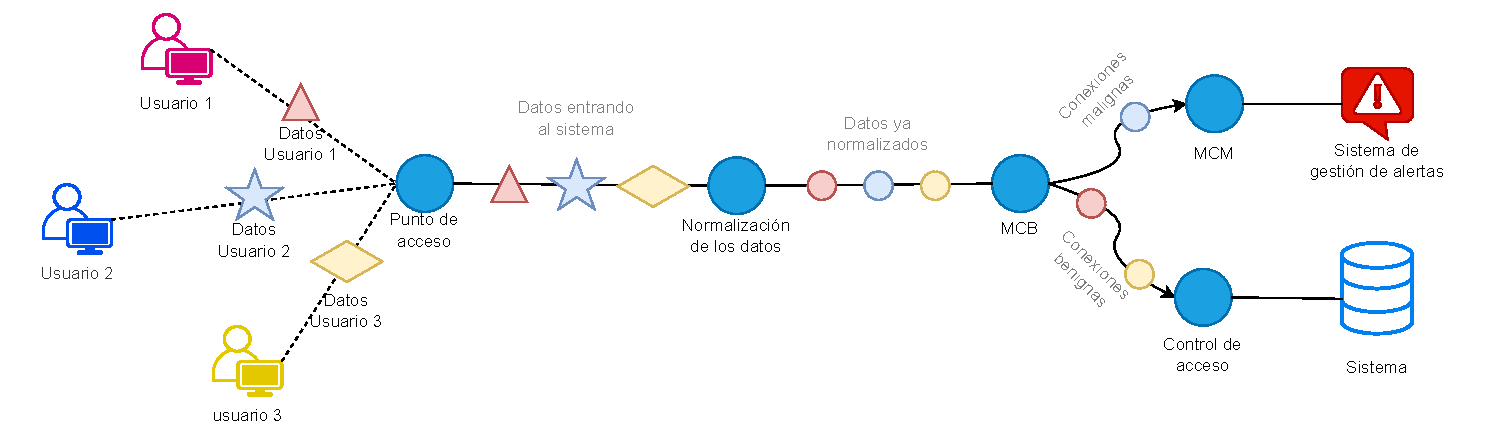
\includegraphics[width=1\textwidth]{../Memoria/img/despliegue/despliegue.pdf}
    \caption{Ejemplo de despliegue de los modelos en un sistema informático.}
    \label{fig:despliegue}
\end{figure}

\end{frame}


\chapter{Tecnologías usadas}



\chapter{Seguimiento del proyecto}\label{cap:seguimiento}



\chapter{Conclusiones}

En este capítulo se exponen las conclusiones derivadas del desarrollo y evaluación del modelo neuronal diseñado para la clasificación de conexiones benignas y malignas. El enfoque propuesto consiste en un modelo de clasificación binaria que, una vez realiza la distinción entre conexiones benignas y malignas, redirige aquellas conexiones clasificadas como malignas hacia un modelo de clasificación multiclase. Este último modelo es capaz de diferenciar las conexiones malignas en nueve clases distintas, permitiendo una identificación más detallada y precisa de los diversos tipos de intrusiones. Los resultados obtenidos destacan la eficacia de ambos modelos, evidenciando su capacidad para abordar de manera jerárquica y especializada la clasificación. Finalmente, se presentan las limitaciones del estudio y se plantean posibles líneas de trabajo futuro.

\section{Conclusiones}

El primer objetivo del proyecto, consistente en diseñar e implementar un modelo capaz de detectar intrusiones en redes informáticas y proporcionar una clasificación preliminar de las mismas, se ha cubierto de forma satisfactoria. Este primer objetivo del proyecto se ha alcanzado al obtener un modelo de clasificación binaria capaz de distinguir entre conexiones benignas y malignas con un \textit{Recall} superior a $0.99$. Con respecto a la clasificación de intrusiones o conexiones malignas, se ha desarrollado un modelo de clasificación multiclase, que recibe las conexiones clasificadas por el modelo binario como malignas y clasifica estas conexiones en nueve clases diferentes de intrusiones en sistemas informáticos con un \textit{F1-weighted} cercano a $0.6$.

El segundo objetivo del proyecto, según el cual los modelos de detección debían ser modelos neuronales, se ha alcanzado satisfactoriamente. Este objetivo se logró mediante el diseño de modelos de clasificación binaria (MsCB) y multiclase (MsCM), ambos con una arquitectura compuesta por dos capas. La primera de las capas en todos los modelos corresponde con la capa oculta, es la capa que recibe los atributos de entrada del modelo y la que permite que se pueda resolver el problema no lineal que se propone en este trabajo. Esta primera capa cuenta con un número diferente de neuronas en función de la arquitectura del modelo que se observe. La segunda capa por su parte, es la que corresponde con la salida del modelo. Esta segunda capa cuenta con una única neurona en el caso de los MsCB y con nueve neuronas en el caso de los MsCM.  La utilización de un Perceptrón Multicapa (MLP) en ambos modelos de clasificación permite aprovechar la capacidad de las redes neuronales para aprender representaciones complejas y no lineales, mejorando la capacidad de clasificación

El tercer objetivo del proyecto, consistente en evaluar y comparar los modelos generados utilizando un conjunto de datos real y complejo, se ha alcanzado de manera adecuada. Tal y como se expone en el Capítulo \ref{cap.ent-datos}, correspondiente a la fase de entendimiento de los datos de la metodología CRISP-DM, el conjunto de datos empleado para dicha evaluación ha sido el \texttt{NF-UNSW-NB15-v3}. \cite{luay2025NetFlowDatasetsV3}. Este conjunto de datos es semi-sintético, esto se debe a que los flujos benignos son registros reales de la conexión entre dos sistemas, mientras que los flujos correspondientes a los ataques se generaron en un entorno controlado. Para evitar que los datos sintéticos de los flujos maliciosos perjudicasen el entrenamiento y la evaluación de los modelos, se transformaron los datos, eliminando aquellos atributos que presentaban valores que diferían con la realidad, como fue el caso de las direcciones IP.

Evaluar el grado en el que se han alcanzado los objetivos académicos es más complejo que evaluar si los objetivos del proyecto se han conseguido cumplir. Esta diferencia se debe a que mientras que los objetivos del proyecto son medibles cuantitativamente, los objeticos académicos no son medibles objetivamente. Sin embargo, teniendo en cuenta el trabajo desarrollado se considera que si se han alcanzado todos los objetivos académicos fijados.

El primer objetivo académico, centrado en comprender el funcionamiento de los modelos neuronales mediante \texttt{PyTorch} y las métricas de evaluación, se ha abordado a lo largo del desarrollo del proyecto. Al haber desarrollado varios modelos con difertes arquitecturas y calcular las métricas tanto de la fase de validación como de la fase de evaluación utilizando la biblioteca \texttt{PyTorch}, se puede afirmar que se ha comprendido el funcionamiendo de los modelos neuronales, alcanzando de esta manera el primer objetivo académico.

El segundo objetivo académico, consiste en aprender las características de varios de los tipo de modelos neruonales que existen, se ha alcanzado de manera satisfactoria. En la sección \ref{subsec.tiposmodel} del capítulo \ref{cap.modelos}, se explican algunos de los modelos neuronales que más se utilizan en la actualidad y se comentan las caracterísitcas de cada tipo de modelo, proporcionando una visión de las tareas en las que mejor desempeño muestra cada tipo. Tras analizar las características de los diferentes tipos de modelos neuronales, se determinó que el Perceptrón Multicapa (MLP) era la opción más adecuada para este problema, dado que los datos presentan una naturaleza no lineal y el MLP tiene la capacidad de aprender representaciones complejas y no lineales, lo cual resulta fundamental para resolver este tipo de clasificación. Para redactar la sección mencionada fue necesario entender cuales eran las caraterísticas de cada tipo de modelo neuronal, por lo que el segundo objetivo académico se ha cumplido correctamente durante el desarrollo de este trabajo.

El tercer objetivo académico, se centra en descubrir el potencial de las redes neuronales para optimizar y mejorar las tecnologías de la información, incluyendo la ciberseguridad de los sistemas, se ha cubiertod de manera satisfactoria . Tras el desarrollo de este trabajo se ha descubierto que los modelos neuronales tienen una gran capacidad para resolver problemas de clasificación con una complejidad elevada. Además, resulta fascinante el hecho de que los pesos de las neuronas se puedan ajustar en cualquier momento para converger hacia una solución más generalizada o precisa del problema. Esta capacidad de adaptación es esencial en las tecnologías de la información, y en especial en la ciberseguridad ya que es un campo que se encuentra en constante evolución. Teniendo esto en cuenta, no solo se ha descubierto el potencial de las redes neuronales para optimizar y mejorar las tecnologías de la información, incluyendo la ciberseguridad de los sistemas, si no que además se ha descubierto el potencial que tienen las redes neuronales para resolver problemas complejos y su alta capacidad de adaptación a cambios en el problema que resuelven.

%Puesto que se han completado todos los objetivos del proyecto, así como los objetivos académicos fijados al comienzo de la memoria, se puede afirmar que el trabajo ha sido un éxito. Se ha desarrollado un modelo capaz de detectar intrusiones en sistemas informáticos y clasificarlas en nueve tipos diferentes de intrusiones. Además, se han obtenido conocimientos acerca de las redes neuronales que se ignoraban por parte del alumno antes del desarrollo de este trabajo.


\section{Trabajo futuro}
En un posible trabajo futuro se podría explorar como afecta el uso de las técnicas que se comentan en esta sección en la eficacia y en la eficiencia de los modelos desarrollados, con el objetivo de obtener modelos que convejan hacia una solución que generalice mejor, especialmente en el modelo de clasificación multiclase.

\begin{itemize}
	\item Modificar la arquitectura del modelo de clasificación multiclase. Durante el desarrollo del trabajo se han comparado los resultados que se obtenían al modificar el tamaño de la capa oculta. Estas comparaciones han demostrado que en función de la complejidad del problema aumentar el número de neuronas puede ser beneficioso o contraproducente. También se ha probado a añadir una tercera capa en el modelo de clasificación multiclase para comprobar si aplicando esta técnica, el modelo conseguía compensar el desbalanceo en el número de muestras de algunas clases del conjunto de datos con la complejidad de la red neuronal. Desafortunadamente, el valor más alto obtenido en la métrica \textit{F1-weighted} utilizando una arquitectura de tres capas, no superó los resultados obtenidos por los modelos con dos capas.
	
	Sin embargo, al modificar la arquitectura del modelo de clasificación multiclase, sería posible lograr que el modelo converja hacia una solución que sea capaz de identificar con una mayor exactitud aquellas clases con un menor número de muestras, mejorando de esta manera la probabilidad de identificar tanto las clases minoritarias como las mayoritarias.
	
	\item Balancear las clases que identifica el modelo de clasificación multiclase añadiendo nuevos datos al conjunto de datos utilizado durante la fase de entrenamiento. Como se ha comentado en varias ocasiones, el conjunto de datos utilizado durante el entrenamiento de los modelos tiene una proporción realista entre los datos de las conexiones que lo conforman. Que el conjunto de datos presente esta característica es fundamental para comprobar cual sería el comportamiento del modelo en un entorno de producción real. El aspecto negativo, es que en la realidad no existe un equilibrio entre los tipos de intrusiones que sufre un sistema informático, por lo que los datos se encuentran extremadamente desbalanceados.
	
	Al utilizar datos balanceados durante la fase de entrenamiento del modelo y datos realistas durante la fase de evaluación del mismo, se obtendría un modelo capaz de distinguir mejor entre las nueve clases de intrusiones que se tratan en este trabajo y se podría comprobar la eficacia real del modelo de clasificación multiclase al evaluarlo con un conjunto de datos que representan de manera más fideligna las intrusiones que puede sufir un sistema informático.
	
	\item Desplegar los modelos para integrarlos en entornos operativos. Tal y como se comenta en el capítulo \ref{cap.despliegue}, desplegar los modelos contribuiría a mejorar la seguridad en redes mediante la automatización de la detección de conexiones malignas, como sucede con los IDS. Una vez detectada la actividad maliciosa, se podría dar respuestas rápidas a las intrusiones para mitigar sus efectos, como hacen los IPS.
	
	\item Entenar los modelos con los datos que estos reciben una vez desplegados. En las secciones anteriores se comenta que una de las ventajas de utilizar modelos neuronales para la detección de intrusiones en vez de algoritmos, es la capacidad de los modelos de aprender de las conexiones que reciben mientras están en producción y su potencial para detectar patrones no lineales que pueden presentar nuevos tipos de ataques desconocidos como los \textit{zero day}.
	
	\item Comparar los resultados obtenidos con los resultados de articulos publicaciones que utilicen el mismo \textit{dataset} o traten el tema de manera similar. Contrastar los resultados obtenidos con estudios previos que emplean el mismo dataset o abordan problemáticas similares permite evaluar objetivamente el desempeño del enfoque propuesto. Esta práctica no solo aporta rigor científico al análisis, sino que también facilita la identificación de avances, limitaciones y oportunidades de mejora en relación con investigaciones existentes.
\end{itemize}




\appendix

\chapter{Manuales}\label{aped.A}

\section{Manual de despliegue e instalación} 


\section{Manual de mantenimiento}



\section{Manual de usuario}



\chapter{Resumen de enlaces adicionales}\label{aped.B}
\label{anexoenlaces}
Los enlaces útiles de interés en este Trabajo Fin de Grado son:

\begin{itemize}
    \item Repositorio del código: \url{https://gitlab.inf.uva.es/}.

\end{itemize}
 


%Esto es una cita: \cite{ej}. Tiene que hacer referencia a la etiqueta de un bibitem.

%Esto es un enlace \href{www.enlace.net}{Enlace}

% Esto es una url \url{http://www.uva.es}


\cleardoublepage
\addcontentsline{toc}{chapter}{Bibliografía}
%\renewcommand\bibname{Referencias Web}
 %\begin{thebibliography}{X}

 %\bibitem{velostat} \textit{Velostat}, \\
 %\textsc{ejemplo.com}.
 %\\Recuperado a tal fecha, \\de \href{http://ejemplo.com}
 %\end{thebibliography}
 
%\nocite{*}
\bibliographystyle{unsrt}
\bibliography{bibliografia}


\end{document}
